\documentclass[twoside]{book}

% Packages required by doxygen
\usepackage{fixltx2e}
\usepackage{calc}
\usepackage{doxygen}
\usepackage[export]{adjustbox} % also loads graphicx
\usepackage{graphicx}
\usepackage[utf8]{inputenc}
\usepackage{makeidx}
\usepackage{multicol}
\usepackage{multirow}
\PassOptionsToPackage{warn}{textcomp}
\usepackage{textcomp}
\usepackage[nointegrals]{wasysym}
\usepackage[table]{xcolor}

% Font selection
\usepackage[T1]{fontenc}
\usepackage[scaled=.90]{helvet}
\usepackage{courier}
\usepackage{amssymb}
\usepackage{sectsty}
\renewcommand{\familydefault}{\sfdefault}
\allsectionsfont{%
  \fontseries{bc}\selectfont%
  \color{darkgray}%
}
\renewcommand{\DoxyLabelFont}{%
  \fontseries{bc}\selectfont%
  \color{darkgray}%
}
\newcommand{\+}{\discretionary{\mbox{\scriptsize$\hookleftarrow$}}{}{}}

% Page & text layout
\usepackage{geometry}
\geometry{%
  a4paper,%
  top=2.5cm,%
  bottom=2.5cm,%
  left=2.5cm,%
  right=2.5cm%
}
\tolerance=750
\hfuzz=15pt
\hbadness=750
\setlength{\emergencystretch}{15pt}
\setlength{\parindent}{0cm}
\setlength{\parskip}{3ex plus 2ex minus 2ex}
\makeatletter
\renewcommand{\paragraph}{%
  \@startsection{paragraph}{4}{0ex}{-1.0ex}{1.0ex}{%
    \normalfont\normalsize\bfseries\SS@parafont%
  }%
}
\renewcommand{\subparagraph}{%
  \@startsection{subparagraph}{5}{0ex}{-1.0ex}{1.0ex}{%
    \normalfont\normalsize\bfseries\SS@subparafont%
  }%
}
\makeatother

% Headers & footers
\usepackage{fancyhdr}
\pagestyle{fancyplain}
\fancyhead[LE]{\fancyplain{}{\bfseries\thepage}}
\fancyhead[CE]{\fancyplain{}{}}
\fancyhead[RE]{\fancyplain{}{\bfseries\leftmark}}
\fancyhead[LO]{\fancyplain{}{\bfseries\rightmark}}
\fancyhead[CO]{\fancyplain{}{}}
\fancyhead[RO]{\fancyplain{}{\bfseries\thepage}}
\fancyfoot[LE]{\fancyplain{}{}}
\fancyfoot[CE]{\fancyplain{}{}}
\fancyfoot[RE]{\fancyplain{}{\bfseries\scriptsize Generated by Doxygen }}
\fancyfoot[LO]{\fancyplain{}{\bfseries\scriptsize Generated by Doxygen }}
\fancyfoot[CO]{\fancyplain{}{}}
\fancyfoot[RO]{\fancyplain{}{}}
\renewcommand{\footrulewidth}{0.4pt}
\renewcommand{\chaptermark}[1]{%
  \markboth{#1}{}%
}
\renewcommand{\sectionmark}[1]{%
  \markright{\thesection\ #1}%
}

% Indices & bibliography
\usepackage{natbib}
\usepackage[titles]{tocloft}
\setcounter{tocdepth}{3}
\setcounter{secnumdepth}{5}
\makeindex

% Hyperlinks (required, but should be loaded last)
\usepackage{ifpdf}
\ifpdf
  \usepackage[pdftex,pagebackref=true]{hyperref}
\else
  \usepackage[ps2pdf,pagebackref=true]{hyperref}
\fi
\hypersetup{%
  colorlinks=true,%
  linkcolor=blue,%
  citecolor=blue,%
  unicode%
}

% Custom commands
\newcommand{\clearemptydoublepage}{%
  \newpage{\pagestyle{empty}\cleardoublepage}%
}

\usepackage{caption}
\captionsetup{labelsep=space,justification=centering,font={bf},singlelinecheck=off,skip=4pt,position=top}

%===== C O N T E N T S =====

\begin{document}

% Titlepage & ToC
\hypersetup{pageanchor=false,
             bookmarksnumbered=true,
             pdfencoding=unicode
            }
\pagenumbering{alph}
\begin{titlepage}
\vspace*{7cm}
\begin{center}%
{\Large Geometry Processing library \\[1ex]\large 2018-\/2019\+Q1 }\\
\vspace*{1cm}
{\large Generated by Doxygen 1.8.13}\\
\end{center}
\end{titlepage}
\clearemptydoublepage
\pagenumbering{roman}
\tableofcontents
\clearemptydoublepage
\pagenumbering{arabic}
\hypersetup{pageanchor=true}

%--- Begin generated contents ---
\chapter{Namespace Index}
\section{Namespace List}
Here is a list of all documented namespaces with brief descriptions\+:\begin{DoxyCompactList}
\item\contentsline{section}{\hyperlink{namespacegeoproc}{geoproc} \\*Main namespace of the library }{\pageref{namespacegeoproc}}{}
\item\contentsline{section}{\hyperlink{namespacegeoproc_1_1curvature}{geoproc\+::curvature} \\*Implementation of different curvature algorithms }{\pageref{namespacegeoproc_1_1curvature}}{}
\item\contentsline{section}{\hyperlink{namespacegeoproc_1_1filter__frequencies}{geoproc\+::filter\+\_\+frequencies} \\*Frequencies filtering }{\pageref{namespacegeoproc_1_1filter__frequencies}}{}
\item\contentsline{section}{\hyperlink{namespacegeoproc_1_1iterators}{geoproc\+::iterators} \\*Classes used as iterators over features of a triangular mesh }{\pageref{namespacegeoproc_1_1iterators}}{}
\item\contentsline{section}{\hyperlink{namespacegeoproc_1_1iterators_1_1vertex}{geoproc\+::iterators\+::vertex} \\*Iterate over vertices }{\pageref{namespacegeoproc_1_1iterators_1_1vertex}}{}
\item\contentsline{section}{\hyperlink{namespacegeoproc_1_1parametrisation}{geoproc\+::parametrisation} \\*Parametrisation algorithms }{\pageref{namespacegeoproc_1_1parametrisation}}{}
\item\contentsline{section}{\hyperlink{namespacegeoproc_1_1PLY__reader}{geoproc\+::\+P\+L\+Y\+\_\+reader} \\*Read a mesh in .ply format }{\pageref{namespacegeoproc_1_1PLY__reader}}{}
\item\contentsline{section}{\hyperlink{namespacegeoproc_1_1remeshing}{geoproc\+::remeshing} \\*Remeshing algorithms }{\pageref{namespacegeoproc_1_1remeshing}}{}
\item\contentsline{section}{\hyperlink{namespacegeoproc_1_1smoothing}{geoproc\+::smoothing} \\*Implementation of different smoothing algorithms }{\pageref{namespacegeoproc_1_1smoothing}}{}
\item\contentsline{section}{\hyperlink{namespacegeoproc_1_1smoothing_1_1global}{geoproc\+::smoothing\+::global} \\*Global smoothing algorithms }{\pageref{namespacegeoproc_1_1smoothing_1_1global}}{}
\item\contentsline{section}{\hyperlink{namespacegeoproc_1_1smoothing_1_1local}{geoproc\+::smoothing\+::local} \\*Local smoothing algorithms }{\pageref{namespacegeoproc_1_1smoothing_1_1local}}{}
\item\contentsline{section}{\hyperlink{namespacegeoproc_1_1smoothing_1_1local__private}{geoproc\+::smoothing\+::local\+\_\+private} \\*Local smoothing algorithms core functions }{\pageref{namespacegeoproc_1_1smoothing_1_1local__private}}{}
\end{DoxyCompactList}

\chapter{Hierarchical Index}
\section{Class Hierarchy}
This inheritance list is sorted roughly, but not completely, alphabetically\+:\begin{DoxyCompactList}
\item \contentsline{section}{geoproc\+:\+:mesh\+\_\+edge}{\pageref{classgeoproc_1_1mesh__edge}}{}
\item \contentsline{section}{geoproc\+:\+:iterators\+:\+:mesh\+\_\+iterator}{\pageref{classgeoproc_1_1iterators_1_1mesh__iterator}}{}
\begin{DoxyCompactList}
\item \contentsline{section}{geoproc\+:\+:iterators\+:\+:vertex\+:\+:vertex\+\_\+face\+\_\+iterator}{\pageref{classgeoproc_1_1iterators_1_1vertex_1_1vertex__face__iterator}}{}
\item \contentsline{section}{geoproc\+:\+:iterators\+:\+:vertex\+:\+:vertex\+\_\+vertex\+\_\+iterator}{\pageref{classgeoproc_1_1iterators_1_1vertex_1_1vertex__vertex__iterator}}{}
\end{DoxyCompactList}
\item \contentsline{section}{geoproc\+:\+:filter\+\_\+frequencies\+:\+:smoothing\+\_\+configuration}{\pageref{structgeoproc_1_1filter__frequencies_1_1smoothing__configuration}}{}
\item \contentsline{section}{geoproc\+:\+:Triangle\+Mesh}{\pageref{classgeoproc_1_1TriangleMesh}}{}
\end{DoxyCompactList}

\chapter{Class Index}
\section{Class List}
Here are the classes, structs, unions and interfaces with brief descriptions\+:\begin{DoxyCompactList}
\item\contentsline{section}{\hyperlink{classgeoproc_1_1mesh__edge}{geoproc\+::mesh\+\_\+edge} \\*Meshe\textquotesingle{}s edge defition }{\pageref{classgeoproc_1_1mesh__edge}}{}
\item\contentsline{section}{\hyperlink{classgeoproc_1_1iterators_1_1mesh__iterator}{geoproc\+::iterators\+::mesh\+\_\+iterator} \\*Abstract iterator class }{\pageref{classgeoproc_1_1iterators_1_1mesh__iterator}}{}
\item\contentsline{section}{\hyperlink{structgeoproc_1_1filter__frequencies_1_1smoothing__configuration}{geoproc\+::filter\+\_\+frequencies\+::smoothing\+\_\+configuration} \\*A smoothing algorithm configuration }{\pageref{structgeoproc_1_1filter__frequencies_1_1smoothing__configuration}}{}
\item\contentsline{section}{\hyperlink{classgeoproc_1_1TriangleMesh}{geoproc\+::\+Triangle\+Mesh} \\*Implementation of a triangular mesh }{\pageref{classgeoproc_1_1TriangleMesh}}{}
\item\contentsline{section}{\hyperlink{classgeoproc_1_1iterators_1_1vertex_1_1vertex__face__iterator}{geoproc\+::iterators\+::vertex\+::vertex\+\_\+face\+\_\+iterator} \\*Face iterator class }{\pageref{classgeoproc_1_1iterators_1_1vertex_1_1vertex__face__iterator}}{}
\item\contentsline{section}{\hyperlink{classgeoproc_1_1iterators_1_1vertex_1_1vertex__vertex__iterator}{geoproc\+::iterators\+::vertex\+::vertex\+\_\+vertex\+\_\+iterator} \\*Vertex iterator class }{\pageref{classgeoproc_1_1iterators_1_1vertex_1_1vertex__vertex__iterator}}{}
\end{DoxyCompactList}

\chapter{Namespace Documentation}
\hypertarget{namespacegeoproc}{}\section{geoproc Namespace Reference}
\label{namespacegeoproc}\index{geoproc@{geoproc}}


Main namespace of the library.  


\subsection*{Namespaces}
\begin{DoxyCompactItemize}
\item 
 \hyperlink{namespacegeoproc_1_1curvature}{curvature}
\begin{DoxyCompactList}\small\item\em Implementation of different curvature algorithms. \end{DoxyCompactList}\item 
 \hyperlink{namespacegeoproc_1_1filter__frequencies}{filter\+\_\+frequencies}
\begin{DoxyCompactList}\small\item\em Frequencies filtering. \end{DoxyCompactList}\item 
 \hyperlink{namespacegeoproc_1_1iterators}{iterators}
\begin{DoxyCompactList}\small\item\em Classes used as iterators over features of a triangular mesh. \end{DoxyCompactList}\item 
 \hyperlink{namespacegeoproc_1_1parametrisation}{parametrisation}
\begin{DoxyCompactList}\small\item\em Parametrisation algorithms. \end{DoxyCompactList}\item 
 \hyperlink{namespacegeoproc_1_1PLY__reader}{P\+L\+Y\+\_\+reader}
\begin{DoxyCompactList}\small\item\em Read a mesh in .ply format. \end{DoxyCompactList}\item 
 \hyperlink{namespacegeoproc_1_1remeshing}{remeshing}
\begin{DoxyCompactList}\small\item\em Remeshing algorithms. \end{DoxyCompactList}\item 
 \hyperlink{namespacegeoproc_1_1smoothing}{smoothing}
\begin{DoxyCompactList}\small\item\em Implementation of different smoothing algorithms. \end{DoxyCompactList}\end{DoxyCompactItemize}
\subsection*{Classes}
\begin{DoxyCompactItemize}
\item 
class \hyperlink{classgeoproc_1_1mesh__edge}{mesh\+\_\+edge}
\begin{DoxyCompactList}\small\item\em Meshe\textquotesingle{}s edge defition. \end{DoxyCompactList}\item 
class \hyperlink{classgeoproc_1_1TriangleMesh}{Triangle\+Mesh}
\begin{DoxyCompactList}\small\item\em Implementation of a triangular mesh. \end{DoxyCompactList}\end{DoxyCompactItemize}
\subsection*{Enumerations}
\begin{DoxyCompactItemize}
\item 
enum \hyperlink{namespacegeoproc_a396280579199558902594f4df72c01c7}{modifier} \+: int8\+\_\+t \{ \hyperlink{namespacegeoproc_a396280579199558902594f4df72c01c7a799723f39baf497704a3d39e7c03555f}{modifier\+::\+Laplacian}, 
\hyperlink{namespacegeoproc_a396280579199558902594f4df72c01c7a0890724bffb79f511bc768c0529dce3f}{modifier\+::\+Bi\+Laplacian}, 
\hyperlink{namespacegeoproc_a396280579199558902594f4df72c01c7ad69ec4945f39affa518f05fa077b00ae}{modifier\+::\+Taubin\+LM}
 \}\begin{DoxyCompactList}\small\item\em The different types of modifiers available. \end{DoxyCompactList}
\item 
enum \hyperlink{namespacegeoproc_a12e5a10581b53b9dd9a509127527f843}{weight} \+: int8\+\_\+t \{ \hyperlink{namespacegeoproc_a12e5a10581b53b9dd9a509127527f843aa489ffed938ef1b9e86889bc413501ee}{weight\+::uniform} = 0, 
\hyperlink{namespacegeoproc_a12e5a10581b53b9dd9a509127527f843a8e8ea879f40475ae2c70be8b296bf950}{weight\+::cotangent}
 \}\begin{DoxyCompactList}\small\item\em The different types of weights. \end{DoxyCompactList}
\item 
enum \hyperlink{namespacegeoproc_a494da744a805b80f842402f0a806ccfc}{boundary\+\_\+shape} \+: int8\+\_\+t \{ \hyperlink{namespacegeoproc_a494da744a805b80f842402f0a806ccfca30954d90085f6eaaf5817917fc5fecb3}{boundary\+\_\+shape\+::\+Circle} = 0, 
\hyperlink{namespacegeoproc_a494da744a805b80f842402f0a806ccfcaceb46ca115d05c51aa5a16a8867c3304}{boundary\+\_\+shape\+::\+Square}
 \}\begin{DoxyCompactList}\small\item\em Shapes for boundary vertices. \end{DoxyCompactList}
\end{DoxyCompactItemize}


\subsection{Detailed Description}
Main namespace of the library. 

In this namespace is defined the main data structure used to implement all the algorithms\+: the \hyperlink{classgeoproc_1_1TriangleMesh}{Triangle\+Mesh}.

In order to read a mesh from disk, see namespace \hyperlink{namespacegeoproc_1_1PLY__reader}{P\+L\+Y\+\_\+reader}.

All the algorithms are defined in their corresponding namespaces. 

\subsection{Enumeration Type Documentation}
\mbox{\Hypertarget{namespacegeoproc_a494da744a805b80f842402f0a806ccfc}\label{namespacegeoproc_a494da744a805b80f842402f0a806ccfc}} 
\index{geoproc@{geoproc}!boundary\+\_\+shape@{boundary\+\_\+shape}}
\index{boundary\+\_\+shape@{boundary\+\_\+shape}!geoproc@{geoproc}}
\subsubsection{\texorpdfstring{boundary\+\_\+shape}{boundary\_shape}}
{\footnotesize\ttfamily enum \hyperlink{namespacegeoproc_a494da744a805b80f842402f0a806ccfc}{geoproc\+::boundary\+\_\+shape} \+: int8\+\_\+t\hspace{0.3cm}{\ttfamily [strong]}}



Shapes for boundary vertices. 

Sometimes we may want to place the vertices at the boundary of a mesh in a certain shape on the xy plane. The shapes are the following\+:
\begin{DoxyItemize}
\item circle\+: see \hyperlink{namespacegeoproc_a494da744a805b80f842402f0a806ccfca30954d90085f6eaaf5817917fc5fecb3}{boundary\+\_\+shape\+::\+Circle}.
\item square\+: see \hyperlink{namespacegeoproc_a494da744a805b80f842402f0a806ccfcaceb46ca115d05c51aa5a16a8867c3304}{boundary\+\_\+shape\+::\+Square}. 
\end{DoxyItemize}\begin{DoxyEnumFields}{Enumerator}
\raisebox{\heightof{T}}[0pt][0pt]{\index{Circle@{Circle}!geoproc@{geoproc}}\index{geoproc@{geoproc}!Circle@{Circle}}}\mbox{\Hypertarget{namespacegeoproc_a494da744a805b80f842402f0a806ccfca30954d90085f6eaaf5817917fc5fecb3}\label{namespacegeoproc_a494da744a805b80f842402f0a806ccfca30954d90085f6eaaf5817917fc5fecb3}} 
Circle&The boundary vertices are placed on the circumference of a circle of radius 1, centered at (0,0). \\
\hline

\raisebox{\heightof{T}}[0pt][0pt]{\index{Square@{Square}!geoproc@{geoproc}}\index{geoproc@{geoproc}!Square@{Square}}}\mbox{\Hypertarget{namespacegeoproc_a494da744a805b80f842402f0a806ccfcaceb46ca115d05c51aa5a16a8867c3304}\label{namespacegeoproc_a494da744a805b80f842402f0a806ccfcaceb46ca115d05c51aa5a16a8867c3304}} 
Square&The boundary vertices are placed on the boundary of a square of side length 2, centered at (0,0). \\
\hline

\end{DoxyEnumFields}
\mbox{\Hypertarget{namespacegeoproc_a396280579199558902594f4df72c01c7}\label{namespacegeoproc_a396280579199558902594f4df72c01c7}} 
\index{geoproc@{geoproc}!modifier@{modifier}}
\index{modifier@{modifier}!geoproc@{geoproc}}
\subsubsection{\texorpdfstring{modifier}{modifier}}
{\footnotesize\ttfamily enum \hyperlink{namespacegeoproc_a396280579199558902594f4df72c01c7}{geoproc\+::modifier} \+: int8\+\_\+t\hspace{0.3cm}{\ttfamily [strong]}}



The different types of modifiers available. 


\begin{DoxyItemize}
\item Laplacian\+: see \hyperlink{namespacegeoproc_a396280579199558902594f4df72c01c7a799723f39baf497704a3d39e7c03555f}{smooth\+\_\+modifier\+::\+Laplacian}.
\item Bi-\/\+Laplacian\+: see \hyperlink{namespacegeoproc_a396280579199558902594f4df72c01c7a0890724bffb79f511bc768c0529dce3f}{smooth\+\_\+modifier\+::\+Bi\+Laplacian}.
\item Taubin\+LM\+: see \hyperlink{namespacegeoproc_a396280579199558902594f4df72c01c7ad69ec4945f39affa518f05fa077b00ae}{smooth\+\_\+modifier\+::\+Taubin\+LM}.
\end{DoxyItemize}

Since \textquotesingle{}operator\textquotesingle{} is a C++\textquotesingle{}s keyword, the word \textquotesingle{}modifier\textquotesingle{} is used instead. \begin{DoxyEnumFields}{Enumerator}
\raisebox{\heightof{T}}[0pt][0pt]{\index{Laplacian@{Laplacian}!geoproc@{geoproc}}\index{geoproc@{geoproc}!Laplacian@{Laplacian}}}\mbox{\Hypertarget{namespacegeoproc_a396280579199558902594f4df72c01c7a799723f39baf497704a3d39e7c03555f}\label{namespacegeoproc_a396280579199558902594f4df72c01c7a799723f39baf497704a3d39e7c03555f}} 
Laplacian&The Laplacian operator on a vertex is formally defined as\+: $ L(v_i) = \sum_{j} w_{ij}(v_j - v_i) $

where $w_{ij}$ is the type of weight. See \hyperlink{namespacegeoproc_a12e5a10581b53b9dd9a509127527f843}{weight} for details.

Its usage is detailed in functions\+:
\begin{DoxyItemize}
\item \hyperlink{namespacegeoproc_1_1smoothing_1_1local_aca304df02cb346b9786b22fa3fb80c88}{smoothing\+::local\+::laplacian(const weight\&, double, size\+\_\+t, Triangle\+Mesh\&)}.
\item \hyperlink{namespacegeoproc_1_1smoothing_1_1local_aeb4e9f73796dce51c4dcac3c1e824fa7}{smoothing\+::local\+::laplacian(const weight\&, double, size\+\_\+t, size\+\_\+t, Triangle\+Mesh\&)}. 
\end{DoxyItemize}\\
\hline

\raisebox{\heightof{T}}[0pt][0pt]{\index{Bi\+Laplacian@{Bi\+Laplacian}!geoproc@{geoproc}}\index{geoproc@{geoproc}!Bi\+Laplacian@{Bi\+Laplacian}}}\mbox{\Hypertarget{namespacegeoproc_a396280579199558902594f4df72c01c7a0890724bffb79f511bc768c0529dce3f}\label{namespacegeoproc_a396280579199558902594f4df72c01c7a0890724bffb79f511bc768c0529dce3f}} 
Bi\+Laplacian&The Bilaplacian operator applies twice the \hyperlink{namespacegeoproc_a396280579199558902594f4df72c01c7a799723f39baf497704a3d39e7c03555f}{modifier\+::\+Laplacian} operator.

Its usage is detailed in functions\+:
\begin{DoxyItemize}
\item \hyperlink{namespacegeoproc_1_1smoothing_1_1local_ae414b9bd00610e2f63096ab8c087b5ea}{smoothing\+::local\+::bilaplacian(const weight\&, double, size\+\_\+t, Triangle\+Mesh\&)}
\item \hyperlink{namespacegeoproc_1_1smoothing_1_1local_a57fc04667cb54871012f162f6af1deed}{smoothing\+::local\+::bilaplacian(const weight\&, double, size\+\_\+t, size\+\_\+t, Triangle\+Mesh\&)} 
\end{DoxyItemize}\\
\hline

\raisebox{\heightof{T}}[0pt][0pt]{\index{Taubin\+LM@{Taubin\+LM}!geoproc@{geoproc}}\index{geoproc@{geoproc}!Taubin\+LM@{Taubin\+LM}}}\mbox{\Hypertarget{namespacegeoproc_a396280579199558902594f4df72c01c7ad69ec4945f39affa518f05fa077b00ae}\label{namespacegeoproc_a396280579199558902594f4df72c01c7ad69ec4945f39affa518f05fa077b00ae}} 
Taubin\+LM&The Taubin\+LM operator applies twice the \hyperlink{namespacegeoproc_a396280579199558902594f4df72c01c7a799723f39baf497704a3d39e7c03555f}{modifier\+::\+Laplacian} operator.

Detailed in the documentation of functions\+:
\begin{DoxyItemize}
\item \hyperlink{namespacegeoproc_1_1smoothing_1_1local_ac234b9f2b455e7dbc97b71bb6c9c47d3}{smoothing\+::local\+::\+Taubin\+L\+M(const weight\&, double, size\+\_\+t, Triangle\+Mesh\&)}
\item \hyperlink{namespacegeoproc_1_1smoothing_1_1local_a05133ca078331bc4fe3e95104c35d3af}{smoothing\+::local\+::\+Taubin\+L\+M(const weight\&, double, size\+\_\+t, size\+\_\+t, Triangle\+Mesh\&)} 
\end{DoxyItemize}\\
\hline

\end{DoxyEnumFields}
\mbox{\Hypertarget{namespacegeoproc_a12e5a10581b53b9dd9a509127527f843}\label{namespacegeoproc_a12e5a10581b53b9dd9a509127527f843}} 
\index{geoproc@{geoproc}!weight@{weight}}
\index{weight@{weight}!geoproc@{geoproc}}
\subsubsection{\texorpdfstring{weight}{weight}}
{\footnotesize\ttfamily enum \hyperlink{namespacegeoproc_a12e5a10581b53b9dd9a509127527f843}{geoproc\+::weight} \+: int8\+\_\+t\hspace{0.3cm}{\ttfamily [strong]}}



The different types of weights. 


\begin{DoxyItemize}
\item uniform\+: see \hyperlink{namespacegeoproc_a12e5a10581b53b9dd9a509127527f843aa489ffed938ef1b9e86889bc413501ee}{weight\+::uniform}.
\item cotangent\+: see \hyperlink{namespacegeoproc_a12e5a10581b53b9dd9a509127527f843a8e8ea879f40475ae2c70be8b296bf950}{weight\+::cotangent}. 
\end{DoxyItemize}\begin{DoxyEnumFields}{Enumerator}
\raisebox{\heightof{T}}[0pt][0pt]{\index{uniform@{uniform}!geoproc@{geoproc}}\index{geoproc@{geoproc}!uniform@{uniform}}}\mbox{\Hypertarget{namespacegeoproc_a12e5a10581b53b9dd9a509127527f843aa489ffed938ef1b9e86889bc413501ee}\label{namespacegeoproc_a12e5a10581b53b9dd9a509127527f843aa489ffed938ef1b9e86889bc413501ee}} 
uniform&Uniform weights. For a vertex $v_i$, the contribution of each vertex of its neighbours $v_j$ is weighted uniformly.

That is, if vertex $v_i$ has $N$ neighbours, the weights are defined as\+:

$ \omega_{ij} = \frac{1}{N} $ \\
\hline

\raisebox{\heightof{T}}[0pt][0pt]{\index{cotangent@{cotangent}!geoproc@{geoproc}}\index{geoproc@{geoproc}!cotangent@{cotangent}}}\mbox{\Hypertarget{namespacegeoproc_a12e5a10581b53b9dd9a509127527f843a8e8ea879f40475ae2c70be8b296bf950}\label{namespacegeoproc_a12e5a10581b53b9dd9a509127527f843a8e8ea879f40475ae2c70be8b296bf950}} 
cotangent&Cotangent weights. For a vertex $v_i$, the contribution of each vertex of its neighbours $v_j$ is weighted using the sum of the cotangents of the angles $ v_i,v_k,v_j $ and . $ v_i,v_l,v_j $, where $ v_k,v_l $ are the two common neighbours of $ v_i,v_j $.

That is, if $ \alpha = \langle v_i,v_k,v_j \rangle $, and $ \beta = \langle v_i,v_l,v_j \rangle $ are the two aforementioned angles, then the weight $ \omega_{ij} $ is defined as\+:

$ \omega_{ij} = \cot(\alpha) + \cot(\beta) $ \\
\hline

\end{DoxyEnumFields}

\hypertarget{namespacegeoproc_1_1curvature}{}\section{geoproc\+:\+:curvature Namespace Reference}
\label{namespacegeoproc_1_1curvature}\index{geoproc\+::curvature@{geoproc\+::curvature}}


Implementation of different curvature algorithms.  


\subsection*{Functions}
\begin{DoxyCompactItemize}
\item 
void \hyperlink{namespacegeoproc_1_1curvature_ac05fe4b3f804678c768241f17f52bb9a}{Gauss} (const \hyperlink{classgeoproc_1_1TriangleMesh}{Triangle\+Mesh} \&mesh, std\+::vector$<$ double $>$ \&Kg, double $\ast$min=nullptr, double $\ast$max=nullptr)
\begin{DoxyCompactList}\small\item\em Computes the Gauss curvature for each vertex. \end{DoxyCompactList}\item 
void \hyperlink{namespacegeoproc_1_1curvature_a769aa493a6028dbd553b6e40711662f8}{Gauss} (const \hyperlink{classgeoproc_1_1TriangleMesh}{Triangle\+Mesh} \&mesh, std\+::vector$<$ double $>$ \&Kg, size\+\_\+t n\+\_\+threads)
\begin{DoxyCompactList}\small\item\em Computes the Gauss curvature for each vertex. \end{DoxyCompactList}\item 
void \hyperlink{namespacegeoproc_1_1curvature_a76b1a28725ce587aec2b5a5d452fb019}{Gauss} (const \hyperlink{classgeoproc_1_1TriangleMesh}{Triangle\+Mesh} \&mesh, std\+::vector$<$ double $>$ \&Kg, size\+\_\+t n\+\_\+threads, double $\ast$min, double $\ast$max)
\begin{DoxyCompactList}\small\item\em Computes the Gauss curvature for each vertex. \end{DoxyCompactList}\item 
void \hyperlink{namespacegeoproc_1_1curvature_a9ccfeae3d3672f6627f4de90bd8ffb0c}{mean} (const \hyperlink{classgeoproc_1_1TriangleMesh}{Triangle\+Mesh} \&mesh, std\+::vector$<$ double $>$ \&Kh, double $\ast$min=nullptr, double $\ast$max=nullptr)
\begin{DoxyCompactList}\small\item\em Computes the mean curvature for each vertex. \end{DoxyCompactList}\item 
void \hyperlink{namespacegeoproc_1_1curvature_a4d1846571b144ee15bd828156bd5f256}{mean} (const \hyperlink{classgeoproc_1_1TriangleMesh}{Triangle\+Mesh} \&mesh, std\+::vector$<$ double $>$ \&Kh, size\+\_\+t n\+\_\+threads)
\begin{DoxyCompactList}\small\item\em Computes the mean curvature for each vertex. \end{DoxyCompactList}\item 
void \hyperlink{namespacegeoproc_1_1curvature_ae649b189f6b14d3dd42fcace8a0e804a}{mean} (const \hyperlink{classgeoproc_1_1TriangleMesh}{Triangle\+Mesh} \&mesh, std\+::vector$<$ double $>$ \&Kh, size\+\_\+t n\+\_\+threads, double $\ast$min, double $\ast$max)
\begin{DoxyCompactList}\small\item\em Computes the mean curvature for each vertex. \end{DoxyCompactList}\end{DoxyCompactItemize}


\subsection{Detailed Description}
Implementation of different curvature algorithms. 

The following curvatures are available\+:
\begin{DoxyItemize}
\item \hyperlink{namespacegeoproc_1_1curvature_ac05fe4b3f804678c768241f17f52bb9a}{curvature\+::\+Gauss(const Triangle\+Mesh\&, std\+::vector$<$double$>$\&, double$\ast$, double$\ast$)}.
\item \hyperlink{namespacegeoproc_1_1curvature_a769aa493a6028dbd553b6e40711662f8}{curvature\+::\+Gauss(const Triangle\+Mesh\&, std\+::vector$<$double$>$\&, size\+\_\+t)}.
\item \hyperlink{namespacegeoproc_1_1curvature_a76b1a28725ce587aec2b5a5d452fb019}{curvature\+::\+Gauss(const Triangle\+Mesh\&, std\+::vector$<$double$>$\&, size\+\_\+t, double$\ast$, double$\ast$)}.
\item \hyperlink{namespacegeoproc_1_1curvature_a9ccfeae3d3672f6627f4de90bd8ffb0c}{curvature\+::mean(const Triangle\+Mesh\&, std\+::vector$<$double$>$\&, double$\ast$, double$\ast$)}.
\item \hyperlink{namespacegeoproc_1_1curvature_a4d1846571b144ee15bd828156bd5f256}{curvature\+::mean(const Triangle\+Mesh\&, std\+::vector$<$double$>$\&, size\+\_\+t)}.
\item \hyperlink{namespacegeoproc_1_1curvature_ae649b189f6b14d3dd42fcace8a0e804a}{curvature\+::mean(const Triangle\+Mesh\&, std\+::vector$<$double$>$\&, size\+\_\+t, double$\ast$, double$\ast$)}. 
\end{DoxyItemize}

\subsection{Function Documentation}
\mbox{\Hypertarget{namespacegeoproc_1_1curvature_ac05fe4b3f804678c768241f17f52bb9a}\label{namespacegeoproc_1_1curvature_ac05fe4b3f804678c768241f17f52bb9a}} 
\index{geoproc\+::curvature@{geoproc\+::curvature}!Gauss@{Gauss}}
\index{Gauss@{Gauss}!geoproc\+::curvature@{geoproc\+::curvature}}
\subsubsection{\texorpdfstring{Gauss()}{Gauss()}\hspace{0.1cm}{\footnotesize\ttfamily [1/3]}}
{\footnotesize\ttfamily void geoproc\+::curvature\+::\+Gauss (\begin{DoxyParamCaption}\item[{const \hyperlink{classgeoproc_1_1TriangleMesh}{Triangle\+Mesh} \&}]{mesh,  }\item[{std\+::vector$<$ double $>$ \&}]{Kg,  }\item[{double $\ast$}]{min = {\ttfamily nullptr},  }\item[{double $\ast$}]{max = {\ttfamily nullptr} }\end{DoxyParamCaption})}



Computes the Gauss curvature for each vertex. 

Use the discretisation of the Laplace-\/\+Beltrami operator, using the cotangents as weights.

This function needs the meshe\textquotesingle{}s angles and areas (see \hyperlink{classgeoproc_1_1TriangleMesh_a4657d7986fd9905c3a7b759e3d1b5442}{Triangle\+Mesh\+::make\+\_\+angles\+\_\+area}). 
\begin{DoxyParams}[1]{Parameters}
 & {\em mesh} & Input mesh. \\
\hline
\mbox{\tt out}  & {\em Kg} & An approximation of the Gauss curvature per vertex. \\
\hline
\mbox{\tt out}  & {\em min} & Minimum curvature value. \\
\hline
\mbox{\tt out}  & {\em max} & Maximum curvature value. \\
\hline
\end{DoxyParams}
\begin{DoxyPrecond}{Precondition}
The mesh requires\+:
\begin{DoxyItemize}
\item Neighbourhood data (see \hyperlink{classgeoproc_1_1TriangleMesh_a84003dfdfd5e591c00f01a797578ff1f}{Triangle\+Mesh\+::make\+\_\+neighbourhood\+\_\+data})
\item Angles and areas (see \hyperlink{classgeoproc_1_1TriangleMesh_a4657d7986fd9905c3a7b759e3d1b5442}{Triangle\+Mesh\+::make\+\_\+angles\+\_\+area}) 
\end{DoxyItemize}
\end{DoxyPrecond}
\mbox{\Hypertarget{namespacegeoproc_1_1curvature_a769aa493a6028dbd553b6e40711662f8}\label{namespacegeoproc_1_1curvature_a769aa493a6028dbd553b6e40711662f8}} 
\index{geoproc\+::curvature@{geoproc\+::curvature}!Gauss@{Gauss}}
\index{Gauss@{Gauss}!geoproc\+::curvature@{geoproc\+::curvature}}
\subsubsection{\texorpdfstring{Gauss()}{Gauss()}\hspace{0.1cm}{\footnotesize\ttfamily [2/3]}}
{\footnotesize\ttfamily void geoproc\+::curvature\+::\+Gauss (\begin{DoxyParamCaption}\item[{const \hyperlink{classgeoproc_1_1TriangleMesh}{Triangle\+Mesh} \&}]{mesh,  }\item[{std\+::vector$<$ double $>$ \&}]{Kg,  }\item[{size\+\_\+t}]{n\+\_\+threads }\end{DoxyParamCaption})}



Computes the Gauss curvature for each vertex. 

Use the discretisation of the Laplace-\/\+Beltrami operator, using the cotangents as weights.

If the number of threads given is 1 then \hyperlink{namespacegeoproc_1_1curvature_ac05fe4b3f804678c768241f17f52bb9a}{Gauss(const Triangle\+Mesh\&, std\+::vector$<$double$>$\&,double$\ast$,double$\ast$)} is called.

This function needs neighbourhood data and the meshe\textquotesingle{}s angles and areas (see \hyperlink{classgeoproc_1_1TriangleMesh_a4657d7986fd9905c3a7b759e3d1b5442}{Triangle\+Mesh\+::make\+\_\+angles\+\_\+area}). 
\begin{DoxyParams}[1]{Parameters}
 & {\em mesh} & Input mesh. \\
\hline
\mbox{\tt out}  & {\em Kg} & An approximation of the Gauss curvature per vertex. \\
\hline
 & {\em n\+\_\+threads} & Number of threads. \\
\hline
\end{DoxyParams}
\begin{DoxyPrecond}{Precondition}
The mesh requires\+:
\begin{DoxyItemize}
\item Neighbourhood data (see \hyperlink{classgeoproc_1_1TriangleMesh_a84003dfdfd5e591c00f01a797578ff1f}{Triangle\+Mesh\+::make\+\_\+neighbourhood\+\_\+data})
\item Angles and areas (see \hyperlink{classgeoproc_1_1TriangleMesh_a4657d7986fd9905c3a7b759e3d1b5442}{Triangle\+Mesh\+::make\+\_\+angles\+\_\+area}) 
\end{DoxyItemize}
\end{DoxyPrecond}
\mbox{\Hypertarget{namespacegeoproc_1_1curvature_a76b1a28725ce587aec2b5a5d452fb019}\label{namespacegeoproc_1_1curvature_a76b1a28725ce587aec2b5a5d452fb019}} 
\index{geoproc\+::curvature@{geoproc\+::curvature}!Gauss@{Gauss}}
\index{Gauss@{Gauss}!geoproc\+::curvature@{geoproc\+::curvature}}
\subsubsection{\texorpdfstring{Gauss()}{Gauss()}\hspace{0.1cm}{\footnotesize\ttfamily [3/3]}}
{\footnotesize\ttfamily void geoproc\+::curvature\+::\+Gauss (\begin{DoxyParamCaption}\item[{const \hyperlink{classgeoproc_1_1TriangleMesh}{Triangle\+Mesh} \&}]{mesh,  }\item[{std\+::vector$<$ double $>$ \&}]{Kg,  }\item[{size\+\_\+t}]{n\+\_\+threads,  }\item[{double $\ast$}]{min,  }\item[{double $\ast$}]{max }\end{DoxyParamCaption})}



Computes the Gauss curvature for each vertex. 

Use the discretisation of the Laplace-\/\+Beltrami operator, using the cotangents as weights.

If the number of threads given is 1 then \hyperlink{namespacegeoproc_1_1curvature_ac05fe4b3f804678c768241f17f52bb9a}{Gauss(const Triangle\+Mesh\&, std\+::vector$<$double$>$\&,double$\ast$,double$\ast$)} is called.

This function needs neighbourhood data and the meshe\textquotesingle{}s angles and areas (see \hyperlink{classgeoproc_1_1TriangleMesh_a4657d7986fd9905c3a7b759e3d1b5442}{Triangle\+Mesh\+::make\+\_\+angles\+\_\+area}). 
\begin{DoxyParams}[1]{Parameters}
 & {\em mesh} & Input mesh. \\
\hline
 & {\em n\+\_\+threads} & Number of threads. \\
\hline
\mbox{\tt out}  & {\em Kg} & An approximation of the Gauss curvature per vertex. \\
\hline
\mbox{\tt out}  & {\em min} & Minimum curvature value. \\
\hline
\mbox{\tt out}  & {\em max} & Maximum curvature value. \\
\hline
\end{DoxyParams}
\begin{DoxyPrecond}{Precondition}
The mesh requires\+:
\begin{DoxyItemize}
\item Neighbourhood data (see \hyperlink{classgeoproc_1_1TriangleMesh_a84003dfdfd5e591c00f01a797578ff1f}{Triangle\+Mesh\+::make\+\_\+neighbourhood\+\_\+data})
\item Angles and areas (see \hyperlink{classgeoproc_1_1TriangleMesh_a4657d7986fd9905c3a7b759e3d1b5442}{Triangle\+Mesh\+::make\+\_\+angles\+\_\+area}) 
\end{DoxyItemize}
\end{DoxyPrecond}
\mbox{\Hypertarget{namespacegeoproc_1_1curvature_a9ccfeae3d3672f6627f4de90bd8ffb0c}\label{namespacegeoproc_1_1curvature_a9ccfeae3d3672f6627f4de90bd8ffb0c}} 
\index{geoproc\+::curvature@{geoproc\+::curvature}!mean@{mean}}
\index{mean@{mean}!geoproc\+::curvature@{geoproc\+::curvature}}
\subsubsection{\texorpdfstring{mean()}{mean()}\hspace{0.1cm}{\footnotesize\ttfamily [1/3]}}
{\footnotesize\ttfamily void geoproc\+::curvature\+::mean (\begin{DoxyParamCaption}\item[{const \hyperlink{classgeoproc_1_1TriangleMesh}{Triangle\+Mesh} \&}]{mesh,  }\item[{std\+::vector$<$ double $>$ \&}]{Kh,  }\item[{double $\ast$}]{min = {\ttfamily nullptr},  }\item[{double $\ast$}]{max = {\ttfamily nullptr} }\end{DoxyParamCaption})}



Computes the mean curvature for each vertex. 

Use the discretisation of the Laplace-\/\+Beltrami operator, using the cotangents as weights.

This function needs neighbourhood data and the meshe\textquotesingle{}s angles and areas (see \hyperlink{classgeoproc_1_1TriangleMesh_a4657d7986fd9905c3a7b759e3d1b5442}{Triangle\+Mesh\+::make\+\_\+angles\+\_\+area}). 
\begin{DoxyParams}[1]{Parameters}
 & {\em mesh} & Input mesh. \\
\hline
\mbox{\tt out}  & {\em Kh} & An approximation of the mean curvature per vertex. \\
\hline
\mbox{\tt out}  & {\em min} & Minimum curvature value. \\
\hline
\mbox{\tt out}  & {\em max} & Maximum curvature value. \\
\hline
\end{DoxyParams}
\begin{DoxyPrecond}{Precondition}
The mesh requires\+:
\begin{DoxyItemize}
\item Neighbourhood data (see \hyperlink{classgeoproc_1_1TriangleMesh_a84003dfdfd5e591c00f01a797578ff1f}{Triangle\+Mesh\+::make\+\_\+neighbourhood\+\_\+data})
\item Angles and areas (see \hyperlink{classgeoproc_1_1TriangleMesh_a4657d7986fd9905c3a7b759e3d1b5442}{Triangle\+Mesh\+::make\+\_\+angles\+\_\+area}) 
\end{DoxyItemize}
\end{DoxyPrecond}
\mbox{\Hypertarget{namespacegeoproc_1_1curvature_a4d1846571b144ee15bd828156bd5f256}\label{namespacegeoproc_1_1curvature_a4d1846571b144ee15bd828156bd5f256}} 
\index{geoproc\+::curvature@{geoproc\+::curvature}!mean@{mean}}
\index{mean@{mean}!geoproc\+::curvature@{geoproc\+::curvature}}
\subsubsection{\texorpdfstring{mean()}{mean()}\hspace{0.1cm}{\footnotesize\ttfamily [2/3]}}
{\footnotesize\ttfamily void geoproc\+::curvature\+::mean (\begin{DoxyParamCaption}\item[{const \hyperlink{classgeoproc_1_1TriangleMesh}{Triangle\+Mesh} \&}]{mesh,  }\item[{std\+::vector$<$ double $>$ \&}]{Kh,  }\item[{size\+\_\+t}]{n\+\_\+threads }\end{DoxyParamCaption})}



Computes the mean curvature for each vertex. 

Use the discretisation of the Laplace-\/\+Beltrami operator, using the cotangents as weights.

If the number of threads given is 1 then \hyperlink{namespacegeoproc_1_1curvature_a9ccfeae3d3672f6627f4de90bd8ffb0c}{mean(const Triangle\+Mesh\&, std\+::vector$<$double$>$\&,double$\ast$,double$\ast$)} is called.

This function needs neighbourhood data and the meshe\textquotesingle{}s angles and areas (see \hyperlink{classgeoproc_1_1TriangleMesh_a4657d7986fd9905c3a7b759e3d1b5442}{Triangle\+Mesh\+::make\+\_\+angles\+\_\+area}). 
\begin{DoxyParams}[1]{Parameters}
 & {\em mesh} & Input mesh. \\
\hline
\mbox{\tt out}  & {\em Kh} & An approximation of the mean curvature per vertex. \\
\hline
 & {\em n\+\_\+threads} & Number of threads. \\
\hline
\end{DoxyParams}
\begin{DoxyPrecond}{Precondition}
The mesh requires\+:
\begin{DoxyItemize}
\item Neighbourhood data (see \hyperlink{classgeoproc_1_1TriangleMesh_a84003dfdfd5e591c00f01a797578ff1f}{Triangle\+Mesh\+::make\+\_\+neighbourhood\+\_\+data})
\item Angles and areas (see \hyperlink{classgeoproc_1_1TriangleMesh_a4657d7986fd9905c3a7b759e3d1b5442}{Triangle\+Mesh\+::make\+\_\+angles\+\_\+area}) 
\end{DoxyItemize}
\end{DoxyPrecond}
\mbox{\Hypertarget{namespacegeoproc_1_1curvature_ae649b189f6b14d3dd42fcace8a0e804a}\label{namespacegeoproc_1_1curvature_ae649b189f6b14d3dd42fcace8a0e804a}} 
\index{geoproc\+::curvature@{geoproc\+::curvature}!mean@{mean}}
\index{mean@{mean}!geoproc\+::curvature@{geoproc\+::curvature}}
\subsubsection{\texorpdfstring{mean()}{mean()}\hspace{0.1cm}{\footnotesize\ttfamily [3/3]}}
{\footnotesize\ttfamily void geoproc\+::curvature\+::mean (\begin{DoxyParamCaption}\item[{const \hyperlink{classgeoproc_1_1TriangleMesh}{Triangle\+Mesh} \&}]{mesh,  }\item[{std\+::vector$<$ double $>$ \&}]{Kh,  }\item[{size\+\_\+t}]{n\+\_\+threads,  }\item[{double $\ast$}]{min,  }\item[{double $\ast$}]{max }\end{DoxyParamCaption})}



Computes the mean curvature for each vertex. 

Use the discretisation of the Laplace-\/\+Beltrami operator, using the cotangents as weights.

If the number of threads given is 1 then \hyperlink{namespacegeoproc_1_1curvature_a9ccfeae3d3672f6627f4de90bd8ffb0c}{mean(const Triangle\+Mesh\&, std\+::vector$<$double$>$\&,double$\ast$,double$\ast$)} is called.

This function needs neighbourhood data and the meshe\textquotesingle{}s angles and areas (see \hyperlink{classgeoproc_1_1TriangleMesh_a4657d7986fd9905c3a7b759e3d1b5442}{Triangle\+Mesh\+::make\+\_\+angles\+\_\+area}). 
\begin{DoxyParams}[1]{Parameters}
 & {\em mesh} & Input mesh. \\
\hline
 & {\em n\+\_\+threads} & Number of threads. \\
\hline
\mbox{\tt out}  & {\em Kh} & An approximation of the mean curvature per vertex. \\
\hline
\mbox{\tt out}  & {\em min} & Minimum curvature value. \\
\hline
\mbox{\tt out}  & {\em max} & Maximum curvature value. \\
\hline
\end{DoxyParams}
\begin{DoxyPrecond}{Precondition}
The mesh requires\+:
\begin{DoxyItemize}
\item Neighbourhood data (see \hyperlink{classgeoproc_1_1TriangleMesh_a84003dfdfd5e591c00f01a797578ff1f}{Triangle\+Mesh\+::make\+\_\+neighbourhood\+\_\+data})
\item Angles and areas (see \hyperlink{classgeoproc_1_1TriangleMesh_a4657d7986fd9905c3a7b759e3d1b5442}{Triangle\+Mesh\+::make\+\_\+angles\+\_\+area}) 
\end{DoxyItemize}
\end{DoxyPrecond}

\hypertarget{namespacegeoproc_1_1filter__frequencies}{}\section{geoproc\+:\+:filter\+\_\+frequencies Namespace Reference}
\label{namespacegeoproc_1_1filter__frequencies}\index{geoproc\+::filter\+\_\+frequencies@{geoproc\+::filter\+\_\+frequencies}}


Frequencies filtering.  


\subsection*{Classes}
\begin{DoxyCompactItemize}
\item 
struct \hyperlink{structgeoproc_1_1filter__frequencies_1_1smoothing__configuration}{smoothing\+\_\+configuration}
\begin{DoxyCompactList}\small\item\em A smoothing algorithm configuration. \end{DoxyCompactList}\end{DoxyCompactItemize}
\subsection*{Functions}
\begin{DoxyCompactItemize}
\item 
void \hyperlink{namespacegeoproc_1_1filter__frequencies_aa795010d1cd2daaafb0b1f60ee3ab1cd}{band\+\_\+frequencies} (const std\+::vector$<$ \hyperlink{structgeoproc_1_1filter__frequencies_1_1smoothing__configuration}{smoothing\+\_\+configuration} $>$ \&confs, const std\+::vector$<$ float $>$ \&mus, \hyperlink{classgeoproc_1_1TriangleMesh}{Triangle\+Mesh} \&m)
\begin{DoxyCompactList}\small\item\em Band frequencies operator. \end{DoxyCompactList}\item 
void \hyperlink{namespacegeoproc_1_1filter__frequencies_a2af31b5e6e8c4d0f5de51c488c1d69b2}{band\+\_\+frequencies} (const std\+::vector$<$ \hyperlink{structgeoproc_1_1filter__frequencies_1_1smoothing__configuration}{smoothing\+\_\+configuration} $>$ \&confs, const std\+::vector$<$ float $>$ \&mus, size\+\_\+t nt, \hyperlink{classgeoproc_1_1TriangleMesh}{Triangle\+Mesh} \&m)
\begin{DoxyCompactList}\small\item\em Band frequencies operator. \end{DoxyCompactList}\end{DoxyCompactItemize}


\subsection{Detailed Description}
Frequencies filtering. 

Implementation of algorithms to highlight certain frequencies of a mesh. 

\subsection{Function Documentation}
\mbox{\Hypertarget{namespacegeoproc_1_1filter__frequencies_aa795010d1cd2daaafb0b1f60ee3ab1cd}\label{namespacegeoproc_1_1filter__frequencies_aa795010d1cd2daaafb0b1f60ee3ab1cd}} 
\index{geoproc\+::filter\+\_\+frequencies@{geoproc\+::filter\+\_\+frequencies}!band\+\_\+frequencies@{band\+\_\+frequencies}}
\index{band\+\_\+frequencies@{band\+\_\+frequencies}!geoproc\+::filter\+\_\+frequencies@{geoproc\+::filter\+\_\+frequencies}}
\subsubsection{\texorpdfstring{band\+\_\+frequencies()}{band\_frequencies()}\hspace{0.1cm}{\footnotesize\ttfamily [1/2]}}
{\footnotesize\ttfamily void geoproc\+::filter\+\_\+frequencies\+::band\+\_\+frequencies (\begin{DoxyParamCaption}\item[{const std\+::vector$<$ \hyperlink{structgeoproc_1_1filter__frequencies_1_1smoothing__configuration}{smoothing\+\_\+configuration} $>$ \&}]{confs,  }\item[{const std\+::vector$<$ float $>$ \&}]{mus,  }\item[{\hyperlink{classgeoproc_1_1TriangleMesh}{Triangle\+Mesh} \&}]{m }\end{DoxyParamCaption})}



Band frequencies operator. 

Apply several smoothing operations onto the mesh {\itshape m}. Each operation is described by a \hyperlink{structgeoproc_1_1filter__frequencies_1_1smoothing__configuration}{smoothing\+\_\+configuration} struct.

The operations applied are\+:

$M + \sum_{i=1}^n \mu_i \cdot D_i$

where each $D_i$ is the difference of meshes resulting from two consecutive smoothing operations (or band frequency), and $\mu_i$ are the weights for each band frequency.

The band frequencies $D_i$ are more precisely defined as\+:

$D_i = S_i(M) - S_{i+1}(M)$,

where $S_i$ is the {\itshape i-\/th} smoothing configuration in parameter {\itshape confs}. Notice, then, that there are $n + 1$ smoothing configurations in {\itshape confs}.


\begin{DoxyParams}[1]{Parameters}
 & {\em confs} & The $S_1,\cdots,S_{n + 1}$ configurations to be applied. \\
\hline
 & {\em mus} & The weights $\mu_1,\cdots,\mu_n$ for each band frequency. \\
\hline
\mbox{\tt out}  & {\em m} & The mesh resulting of applying the operations described above. \\
\hline
\end{DoxyParams}
\begin{DoxyPrecond}{Precondition}
The mesh requires\+:
\begin{DoxyItemize}
\item Neighbourhood data (see \hyperlink{classgeoproc_1_1TriangleMesh_a84003dfdfd5e591c00f01a797578ff1f}{Triangle\+Mesh\+::make\+\_\+neighbourhood\+\_\+data})
\item Angles and areas (see \hyperlink{classgeoproc_1_1TriangleMesh_a4657d7986fd9905c3a7b759e3d1b5442}{Triangle\+Mesh\+::make\+\_\+angles\+\_\+area}) 
\end{DoxyItemize}
\end{DoxyPrecond}
\mbox{\Hypertarget{namespacegeoproc_1_1filter__frequencies_a2af31b5e6e8c4d0f5de51c488c1d69b2}\label{namespacegeoproc_1_1filter__frequencies_a2af31b5e6e8c4d0f5de51c488c1d69b2}} 
\index{geoproc\+::filter\+\_\+frequencies@{geoproc\+::filter\+\_\+frequencies}!band\+\_\+frequencies@{band\+\_\+frequencies}}
\index{band\+\_\+frequencies@{band\+\_\+frequencies}!geoproc\+::filter\+\_\+frequencies@{geoproc\+::filter\+\_\+frequencies}}
\subsubsection{\texorpdfstring{band\+\_\+frequencies()}{band\_frequencies()}\hspace{0.1cm}{\footnotesize\ttfamily [2/2]}}
{\footnotesize\ttfamily void geoproc\+::filter\+\_\+frequencies\+::band\+\_\+frequencies (\begin{DoxyParamCaption}\item[{const std\+::vector$<$ \hyperlink{structgeoproc_1_1filter__frequencies_1_1smoothing__configuration}{smoothing\+\_\+configuration} $>$ \&}]{confs,  }\item[{const std\+::vector$<$ float $>$ \&}]{mus,  }\item[{size\+\_\+t}]{nt,  }\item[{\hyperlink{classgeoproc_1_1TriangleMesh}{Triangle\+Mesh} \&}]{m }\end{DoxyParamCaption})}



Band frequencies operator. 

Apply several smoothing operations onto the mesh {\itshape m}. Each operation is described by a \hyperlink{structgeoproc_1_1filter__frequencies_1_1smoothing__configuration}{smoothing\+\_\+configuration} struct.

The operations applied are\+:

$M + \sum_{i=1}^n \mu_i \cdot D_i$

where each $D_i$ is the difference of meshes resulting from two consecutive smoothing operations (or band frequency), and $\mu_i$ are the weights for each band frequency.

The band frequencies $D_i$ are more precisely defined as\+:

$D_i = S_i(M) - S_{i+1}(M)$,

where $S_i$ is the {\itshape i-\/th} smoothing configuration in parameter {\itshape confs}. Notice, then, that there are $n + 1$ smoothing configurations in {\itshape confs}.


\begin{DoxyParams}[1]{Parameters}
 & {\em confs} & The $S_1,\cdots,S_{n + 1}$ configurations to be applied. \\
\hline
 & {\em mus} & The weights $\mu_1,\cdots,\mu_n$ for each band frequency. \\
\hline
 & {\em nt} & Number of threads. \\
\hline
\mbox{\tt out}  & {\em m} & The mesh resulting of applying the operations described above. \\
\hline
\end{DoxyParams}
\begin{DoxyPrecond}{Precondition}
The mesh requires\+:
\begin{DoxyItemize}
\item Neighbourhood data (see \hyperlink{classgeoproc_1_1TriangleMesh_a84003dfdfd5e591c00f01a797578ff1f}{Triangle\+Mesh\+::make\+\_\+neighbourhood\+\_\+data})
\item Angles and areas (see \hyperlink{classgeoproc_1_1TriangleMesh_a4657d7986fd9905c3a7b759e3d1b5442}{Triangle\+Mesh\+::make\+\_\+angles\+\_\+area}) 
\end{DoxyItemize}
\end{DoxyPrecond}

\hypertarget{namespacegeoproc_1_1iterators}{}\section{geoproc\+:\+:iterators Namespace Reference}
\label{namespacegeoproc_1_1iterators}\index{geoproc\+::iterators@{geoproc\+::iterators}}


Classes used as iterators over features of a triangular mesh.  


\subsection*{Namespaces}
\begin{DoxyCompactItemize}
\item 
 \hyperlink{namespacegeoproc_1_1iterators_1_1vertex}{vertex}
\begin{DoxyCompactList}\small\item\em Iterate over vertices. \end{DoxyCompactList}\end{DoxyCompactItemize}
\subsection*{Classes}
\begin{DoxyCompactItemize}
\item 
class \hyperlink{classgeoproc_1_1iterators_1_1mesh__iterator}{mesh\+\_\+iterator}
\begin{DoxyCompactList}\small\item\em Abstract iterator class. \end{DoxyCompactList}\end{DoxyCompactItemize}


\subsection{Detailed Description}
Classes used as iterators over features of a triangular mesh. 
\hypertarget{namespacegeoproc_1_1iterators_1_1vertex}{}\section{geoproc\+:\+:iterators\+:\+:vertex Namespace Reference}
\label{namespacegeoproc_1_1iterators_1_1vertex}\index{geoproc\+::iterators\+::vertex@{geoproc\+::iterators\+::vertex}}


Iterate over vertices.  


\subsection*{Classes}
\begin{DoxyCompactItemize}
\item 
class \hyperlink{classgeoproc_1_1iterators_1_1vertex_1_1vertex__face__iterator}{vertex\+\_\+face\+\_\+iterator}
\begin{DoxyCompactList}\small\item\em Face iterator class. \end{DoxyCompactList}\item 
class \hyperlink{classgeoproc_1_1iterators_1_1vertex_1_1vertex__vertex__iterator}{vertex\+\_\+vertex\+\_\+iterator}
\begin{DoxyCompactList}\small\item\em Vertex iterator class. \end{DoxyCompactList}\end{DoxyCompactItemize}


\subsection{Detailed Description}
Iterate over vertices. 
\hypertarget{namespacegeoproc_1_1parametrisation}{}\section{geoproc\+:\+:parametrisation Namespace Reference}
\label{namespacegeoproc_1_1parametrisation}\index{geoproc\+::parametrisation@{geoproc\+::parametrisation}}


Parametrisation algorithms.  


\subsection*{Functions}
\begin{DoxyCompactItemize}
\item 
bool \hyperlink{namespacegeoproc_1_1parametrisation_a88891cbeadf541ab81be9333c0c232b3}{harmonic\+\_\+maps} (const \hyperlink{classgeoproc_1_1TriangleMesh}{Triangle\+Mesh} \&m, const \hyperlink{namespacegeoproc_a12e5a10581b53b9dd9a509127527f843}{weight} \&w, const \hyperlink{namespacegeoproc_a494da744a805b80f842402f0a806ccfc}{boundary\+\_\+shape} \&s, std\+::vector$<$ glm\+::vec2 $>$ \&uvs)
\begin{DoxyCompactList}\small\item\em Calculates the texture coordinates using Harmonic Maps. \end{DoxyCompactList}\end{DoxyCompactItemize}


\subsection{Detailed Description}
Parametrisation algorithms. 

Implemented\+:
\begin{DoxyItemize}
\item Harmonic maps (see \hyperlink{namespacegeoproc_1_1parametrisation_a88891cbeadf541ab81be9333c0c232b3}{harmonic\+\_\+maps}). 
\end{DoxyItemize}

\subsection{Function Documentation}
\mbox{\Hypertarget{namespacegeoproc_1_1parametrisation_a88891cbeadf541ab81be9333c0c232b3}\label{namespacegeoproc_1_1parametrisation_a88891cbeadf541ab81be9333c0c232b3}} 
\index{geoproc\+::parametrisation@{geoproc\+::parametrisation}!harmonic\+\_\+maps@{harmonic\+\_\+maps}}
\index{harmonic\+\_\+maps@{harmonic\+\_\+maps}!geoproc\+::parametrisation@{geoproc\+::parametrisation}}
\subsubsection{\texorpdfstring{harmonic\+\_\+maps()}{harmonic\_maps()}}
{\footnotesize\ttfamily bool geoproc\+::parametrisation\+::harmonic\+\_\+maps (\begin{DoxyParamCaption}\item[{const \hyperlink{classgeoproc_1_1TriangleMesh}{Triangle\+Mesh} \&}]{m,  }\item[{const \hyperlink{namespacegeoproc_a12e5a10581b53b9dd9a509127527f843}{weight} \&}]{w,  }\item[{const \hyperlink{namespacegeoproc_a494da744a805b80f842402f0a806ccfc}{boundary\+\_\+shape} \&}]{s,  }\item[{std\+::vector$<$ glm\+::vec2 $>$ \&}]{uvs }\end{DoxyParamCaption})}



Calculates the texture coordinates using Harmonic Maps. 

These coordinates are obtained by solving the linear equation system\+: $Ax = b$ whose construction is similar to that in global smoothing (see \hyperlink{namespacegeoproc_1_1smoothing_1_1global_ac6c034cb72d0a744d0dd843d4df012ff}{smoothing\+::global\+::smooth}).

Matrix {\itshape A} is defined as
\begin{DoxyItemize}
\item $A_{ii} = -1$
\item $A_{ij} = w_{ij}, \forall i \neq j$ where $ 0 \le i,j \le N$.
\end{DoxyItemize}

The values $w_{ij}$ are the weights for vertex $v_i$, and their values depend on parameter {\itshape w}. Matrix $A$ has dimensions $N \times N$, where $N$ is the number of vertices of the mesh. (keep reading to know how fixed vertices are considered...).

The new coordinates of the vertices of the mesh is the solution $x$ of the equation\+:

$Ax_x = b_x$, $Ax_y = b_y$

where $b_x,b_y$ contain some values. When the mesh has one single boundary, its vertices are considered fixed.

The vertices defined as constant are moved to the right hand-\/side of the equation and the matrix of the system becomes $A'$ and has dimensions $v \times v$ where $v$ is the number of variable vertices\+:

$v = N - v^*$, where $v^*$ is the amount of fixed vertices.

The systems are solved using the Simplicial Cholesky method from library Eigen in a least square sense\+:

$ A^TAx_x = A^Tb_x$, $A^TAx_y = A^Tb_y$

In order to save time, the decomposition needed for the Cholesky method is computed only once and reused to solve the three systems defined above.

Now, the Laplacian operator defines the linear equation for vertex $v_i$ as\+:

$L(v_i) = \left(\sum_{j \in N(i)} w_{ij}*v_j\right) - v_i$


\begin{DoxyParams}[1]{Parameters}
 & {\em m} & Input mesh. It must have one single boundary. \\
\hline
 & {\em w} & Type of weights to use to compute the parametrisation. \\
\hline
 & {\em s} & Shape of the boundary vertices on the texture. \\
\hline
\mbox{\tt out}  & {\em uvs} & Texture coordinates of the vertices of {\itshape m} in space \mbox{[}0,0\mbox{]} x \mbox{[}1,1\mbox{]}. \\
\hline
\end{DoxyParams}
\begin{DoxyPrecond}{Precondition}
The mesh requires\+:
\begin{DoxyItemize}
\item Neighbourhood data (see \hyperlink{classgeoproc_1_1TriangleMesh_a84003dfdfd5e591c00f01a797578ff1f}{Triangle\+Mesh\+::make\+\_\+neighbourhood\+\_\+data})
\item Boundaries (see \hyperlink{classgeoproc_1_1TriangleMesh_ad11c9406e2677e4d72d53837206fd769}{Triangle\+Mesh\+::make\+\_\+boundaries})
\item Angles and areas (see \hyperlink{classgeoproc_1_1TriangleMesh_a4657d7986fd9905c3a7b759e3d1b5442}{Triangle\+Mesh\+::make\+\_\+angles\+\_\+area}) 
\end{DoxyItemize}
\end{DoxyPrecond}
\begin{DoxyReturn}{Returns}
Returns true on success. The procedure might fail if there are no boundaries on the mesh or there are more than one. 
\end{DoxyReturn}

\hypertarget{namespacegeoproc_1_1PLY__reader}{}\section{geoproc\+:\+:P\+L\+Y\+\_\+reader Namespace Reference}
\label{namespacegeoproc_1_1PLY__reader}\index{geoproc\+::\+P\+L\+Y\+\_\+reader@{geoproc\+::\+P\+L\+Y\+\_\+reader}}


Read a mesh in .ply format.  


\subsection*{Functions}
\begin{DoxyCompactItemize}
\item 
bool \hyperlink{namespacegeoproc_1_1PLY__reader_a7b13df3c66f0cf33b5ae96ad3302d2e2}{read\+\_\+mesh} (const std\+::string \&filename, \hyperlink{classgeoproc_1_1TriangleMesh}{Triangle\+Mesh} \&mesh)
\begin{DoxyCompactList}\small\item\em Loads a triangular mesh stored in {\itshape filename}. \end{DoxyCompactList}\end{DoxyCompactItemize}


\subsection{Detailed Description}
Read a mesh in .ply format. 

In order to load a mesh in ply format call only function \hyperlink{namespacegeoproc_1_1PLY__reader_a7b13df3c66f0cf33b5ae96ad3302d2e2}{read\+\_\+mesh(const std\+::string\&, Triangle\+Mesh\&)}.

This reader only supports those files that do not contain anything else than vertex coordinates and the description of every face. 

\subsection{Function Documentation}
\mbox{\Hypertarget{namespacegeoproc_1_1PLY__reader_a7b13df3c66f0cf33b5ae96ad3302d2e2}\label{namespacegeoproc_1_1PLY__reader_a7b13df3c66f0cf33b5ae96ad3302d2e2}} 
\index{geoproc\+::\+P\+L\+Y\+\_\+reader@{geoproc\+::\+P\+L\+Y\+\_\+reader}!read\+\_\+mesh@{read\+\_\+mesh}}
\index{read\+\_\+mesh@{read\+\_\+mesh}!geoproc\+::\+P\+L\+Y\+\_\+reader@{geoproc\+::\+P\+L\+Y\+\_\+reader}}
\subsubsection{\texorpdfstring{read\+\_\+mesh()}{read\_mesh()}}
{\footnotesize\ttfamily bool geoproc\+::\+P\+L\+Y\+\_\+reader\+::read\+\_\+mesh (\begin{DoxyParamCaption}\item[{const std\+::string \&}]{filename,  }\item[{\hyperlink{classgeoproc_1_1TriangleMesh}{Triangle\+Mesh} \&}]{mesh }\end{DoxyParamCaption})}



Loads a triangular mesh stored in {\itshape filename}. 


\begin{DoxyParams}[1]{Parameters}
 & {\em filename} & File with the mesh in .ply format. \\
\hline
\mbox{\tt out}  & {\em mesh} & Mesh loaded from file. \\
\hline
\end{DoxyParams}
\begin{DoxyReturn}{Returns}
Returns false on error. 
\end{DoxyReturn}

\hypertarget{namespacegeoproc_1_1remeshing}{}\section{geoproc\+:\+:remeshing Namespace Reference}
\label{namespacegeoproc_1_1remeshing}\index{geoproc\+::remeshing@{geoproc\+::remeshing}}


Remeshing algorithms.  


\subsection*{Functions}
\begin{DoxyCompactItemize}
\item 
bool \hyperlink{namespacegeoproc_1_1remeshing_aaee6fb40eac4d9d9426e4f0f5d15d28c}{harmonic\+\_\+maps} (const \hyperlink{classgeoproc_1_1TriangleMesh}{Triangle\+Mesh} \&m, size\+\_\+t N, size\+\_\+t M, const \hyperlink{namespacegeoproc_1_1smoothing_a76e43f405426c150569712512de58028}{smoothing\+::smooth\+\_\+weight} \&w, const \hyperlink{namespacegeoproc_1_1parametrisation_a7f001bf497830114e8aea2c884a948b7}{parametrisation\+::boundary\+\_\+shape} \&s, \hyperlink{classgeoproc_1_1TriangleMesh}{Triangle\+Mesh} \&rm)
\begin{DoxyCompactList}\small\item\em Remeshes a triangle mesh using harmonic map coordinates. \end{DoxyCompactList}\end{DoxyCompactItemize}


\subsection{Detailed Description}
Remeshing algorithms. 

Implemented\+:
\begin{DoxyItemize}
\item Using Harmonic maps\textquotesingle{} parametrisation (see \hyperlink{namespacegeoproc_1_1remeshing_aaee6fb40eac4d9d9426e4f0f5d15d28c}{harmonic\+\_\+maps}). 
\end{DoxyItemize}

\subsection{Function Documentation}
\mbox{\Hypertarget{namespacegeoproc_1_1remeshing_aaee6fb40eac4d9d9426e4f0f5d15d28c}\label{namespacegeoproc_1_1remeshing_aaee6fb40eac4d9d9426e4f0f5d15d28c}} 
\index{geoproc\+::remeshing@{geoproc\+::remeshing}!harmonic\+\_\+maps@{harmonic\+\_\+maps}}
\index{harmonic\+\_\+maps@{harmonic\+\_\+maps}!geoproc\+::remeshing@{geoproc\+::remeshing}}
\subsubsection{\texorpdfstring{harmonic\+\_\+maps()}{harmonic\_maps()}}
{\footnotesize\ttfamily bool geoproc\+::remeshing\+::harmonic\+\_\+maps (\begin{DoxyParamCaption}\item[{const \hyperlink{classgeoproc_1_1TriangleMesh}{Triangle\+Mesh} \&}]{m,  }\item[{size\+\_\+t}]{N,  }\item[{size\+\_\+t}]{M,  }\item[{const \hyperlink{namespacegeoproc_1_1smoothing_a76e43f405426c150569712512de58028}{smoothing\+::smooth\+\_\+weight} \&}]{w,  }\item[{const \hyperlink{namespacegeoproc_1_1parametrisation_a7f001bf497830114e8aea2c884a948b7}{parametrisation\+::boundary\+\_\+shape} \&}]{s,  }\item[{\hyperlink{classgeoproc_1_1TriangleMesh}{Triangle\+Mesh} \&}]{rm }\end{DoxyParamCaption})}



Remeshes a triangle mesh using harmonic map coordinates. 

First, computes the harmonic maps parametrisation of the mesh, which yields a set of 2d coordinates in the xy plane, more concretely in the square \mbox{[}0,1\mbox{]}x\mbox{[}0,1\mbox{]} (regardless of the shape).

Then, in this square is generated a NxM grid of points. The point $P_{ij}$ (with $0\le i < N, \quad 0\le j < M$) has coordinates $(x(P_{ij}), y(P_{ij})) = (i/N, j/M)$.

Each of these points is located in the triangulation obtained from the parametrisation. That means, that we know the triangle of the triangulation each point of the grid is in.

With this information, for each point in the grid $P_{ij}$, inside triangle $t_k$, the algorithm computes the contribution of the vertices of $t_k$ to make point $P_{ij}$. That is, it computes the weights $w_1,w_2,w_3 > 0, w_1 + w_2 + w_3 = 1$ such that

$ P_{ij} = w_1 \cdot v_1(t_k) + w_2 \cdot v_2(t_k) + w_2 \cdot v_2(t_k) $

where $v_s(t_k)$ is the {\itshape s-\/th} vertex of triangle $t_k$ in the triangulation obtained from the parametrisation.

Once all the $w_i$ are known for each point in the grid, the new mesh is computed\+: a new 3-\/dimensional point is made for each point in the grid, using the weights $w_1,w_2,w_3$ calculated before\+:

$ Q_{ij} = w_1 \cdot v_1(T_k) + w_2 \cdot v_2(T_k) + w_3 \cdot v_3(T_k) $

where $T_k$ denotes the triangle of the original mesh {\itshape m} that is mapped to triangle $t_k$ due to the parametrisation, which is, in turn, the triangle that encloses point $P_{ij}$. 
\begin{DoxyParams}[1]{Parameters}
\mbox{\tt in}  & {\em m} & Triangle mesh to be remeshed. \\
\hline
\mbox{\tt in}  & {\em N} & Size of the grid in the x-\/axis. \\
\hline
\mbox{\tt in}  & {\em M} & Size of the grid in the y-\/axis. \\
\hline
\mbox{\tt in}  & {\em w} & Type of weight to use to obtain the parametrisation. \\
\hline
\mbox{\tt in}  & {\em s} & Boundary shape of the parametrisation. \\
\hline
\mbox{\tt out}  & {\em rm} & Remeshed mesh. \\
\hline
\end{DoxyParams}
\begin{DoxyPrecond}{Precondition}
The input mesh needs all of its edges computed, namely, neighbourhood data has to be valid. 

The preconditions of the method \hyperlink{namespacegeoproc_1_1parametrisation_aa73e02d994e3ef3eba0fcfc5863c8416}{parametrisation\+::harmonic\+\_\+maps} have to be true before calling this method. 
\end{DoxyPrecond}
\begin{DoxyReturn}{Returns}
If method \hyperlink{namespacegeoproc_1_1parametrisation_aa73e02d994e3ef3eba0fcfc5863c8416}{parametrisation\+::harmonic\+\_\+maps} fails (and returns false) this method will return false. Otherwise it will always return true. 
\end{DoxyReturn}

\hypertarget{namespacegeoproc_1_1smoothing}{}\section{geoproc\+:\+:smoothing Namespace Reference}
\label{namespacegeoproc_1_1smoothing}\index{geoproc\+::smoothing@{geoproc\+::smoothing}}


Implementation of different smoothing algorithms.  


\subsection*{Namespaces}
\begin{DoxyCompactItemize}
\item 
 \hyperlink{namespacegeoproc_1_1smoothing_1_1global}{global}
\begin{DoxyCompactList}\small\item\em Global smoothing algorithms. \end{DoxyCompactList}\item 
 \hyperlink{namespacegeoproc_1_1smoothing_1_1local}{local}
\begin{DoxyCompactList}\small\item\em Local smoothing algorithms. \end{DoxyCompactList}\item 
 \hyperlink{namespacegeoproc_1_1smoothing_1_1local__private}{local\+\_\+private}
\begin{DoxyCompactList}\small\item\em Local smoothing algorithms core functions. \end{DoxyCompactList}\end{DoxyCompactItemize}


\subsection{Detailed Description}
Implementation of different smoothing algorithms. 

Iterative, local algorithms, and global algorithms. 
\hypertarget{namespacegeoproc_1_1smoothing_1_1global}{}\section{geoproc\+:\+:smoothing\+:\+:global Namespace Reference}
\label{namespacegeoproc_1_1smoothing_1_1global}\index{geoproc\+::smoothing\+::global@{geoproc\+::smoothing\+::global}}


Global smoothing algorithms.  


\subsection*{Functions}
\begin{DoxyCompactItemize}
\item 
bool \hyperlink{namespacegeoproc_1_1smoothing_1_1global_ac6c034cb72d0a744d0dd843d4df012ff}{smooth} (const \hyperlink{namespacegeoproc_a396280579199558902594f4df72c01c7}{modifier} \&op, const \hyperlink{namespacegeoproc_a12e5a10581b53b9dd9a509127527f843}{weight} \&w, const std\+::vector$<$ bool $>$ \&constant, \hyperlink{classgeoproc_1_1TriangleMesh}{Triangle\+Mesh} \&m)
\begin{DoxyCompactList}\small\item\em Apply a global smoothing algorithm for a given operator and weight. \end{DoxyCompactList}\end{DoxyCompactItemize}


\subsection{Detailed Description}
Global smoothing algorithms. 

\subsection{Function Documentation}
\mbox{\Hypertarget{namespacegeoproc_1_1smoothing_1_1global_ac6c034cb72d0a744d0dd843d4df012ff}\label{namespacegeoproc_1_1smoothing_1_1global_ac6c034cb72d0a744d0dd843d4df012ff}} 
\index{geoproc\+::smoothing\+::global@{geoproc\+::smoothing\+::global}!smooth@{smooth}}
\index{smooth@{smooth}!geoproc\+::smoothing\+::global@{geoproc\+::smoothing\+::global}}
\subsubsection{\texorpdfstring{smooth()}{smooth()}}
{\footnotesize\ttfamily bool geoproc\+::smoothing\+::global\+::smooth (\begin{DoxyParamCaption}\item[{const \hyperlink{namespacegeoproc_a396280579199558902594f4df72c01c7}{modifier} \&}]{op,  }\item[{const \hyperlink{namespacegeoproc_a12e5a10581b53b9dd9a509127527f843}{weight} \&}]{w,  }\item[{const std\+::vector$<$ bool $>$ \&}]{constant,  }\item[{\hyperlink{classgeoproc_1_1TriangleMesh}{Triangle\+Mesh} \&}]{m }\end{DoxyParamCaption})}



Apply a global smoothing algorithm for a given operator and weight. 

This algorithm smoothes a given mesh globally, and in one single step. It defines a system of linear equations, whose matrix is $A$. Such matrix is defined as
\begin{DoxyItemize}
\item $A_{ii} = -1$
\item $A_{ij} = w_{ij}, \forall i \neq j$ where $ 0 \le i,j \le N$.
\end{DoxyItemize}

The values $w_{ij}$ are the weights for vertex $v_i$, and their values depend on parameter {\itshape w}. Matrix $A$ has dimensions $N \times N$, where $N$ is the number of vertices of the mesh. (keep reading to know how fixed vertices are considered...).

The new coordinates of the vertices of the mesh is the solution $x$ of the equation\+:

$Ax_x = b_x$, $Ax_y = b_y$, $Ax_z = b_z$

where $b_x,b_y,b_z$ contain some values. When parameter {\itshape constant} contains no fixed vertices, these vectors will be the zero vector. However, this makes the vertices collapse to the point (0,0,0). Therefore, this algorithm needs some vertices to be set constant (parameter {\itshape constant}).

The vertices defined as constant are moved to the right hand-\/side of the equation and the matrix of the system becomes $A'$ and has dimensions $v \times v$ where $v$ is the number of variable vertices\+:

$v = N - v^*$, where $v^*$ is the amount of fixed vertices in {\itshape constant}.

The systems are solved using the Simplicial Cholesky method from library Eigen in a least square sense\+:

$ A^TAx_x = A^Tb_x$, $A^TAx_y = A^Tb_y$, $A^TAx_z = A^Tb_z$

In order to save time, the decomposition needed for the Cholesky method is computed only once and reused to solve the three systems defined above.

Now, the Laplacian operator defines the linear equation for vertex $v_i$ as\+:

$L(v_i) = \left(\sum_{j \in N(i)} w_{ij}*v_j\right) - v_i$


\begin{DoxyParams}[1]{Parameters}
 & {\em op} & Smoothing operator. \\
\hline
 & {\em w} & Weight type. \\
\hline
 & {\em constant} & {\itshape constant}\mbox{[}i\mbox{]} is true if, and only if, {\itshape i-\/th} vertex is a constant vertex. \\
\hline
\mbox{\tt out}  & {\em m} & Smoothed mesh. \\
\hline
\end{DoxyParams}
\begin{DoxyPrecond}{Precondition}
The mesh requires\+:
\begin{DoxyItemize}
\item Neighbourhood data (see \hyperlink{classgeoproc_1_1TriangleMesh_a84003dfdfd5e591c00f01a797578ff1f}{Triangle\+Mesh\+::make\+\_\+neighbourhood\+\_\+data})
\item Angles and areas (see \hyperlink{classgeoproc_1_1TriangleMesh_a4657d7986fd9905c3a7b759e3d1b5442}{Triangle\+Mesh\+::make\+\_\+angles\+\_\+area}) 
\end{DoxyItemize}

This algorithm is implemented for the following smoothing operators\+:
\begin{DoxyItemize}
\item \hyperlink{namespacegeoproc_a396280579199558902594f4df72c01c7a799723f39baf497704a3d39e7c03555f}{smooth\+\_\+modifier\+::\+Laplacian} 
\end{DoxyItemize}

This algorithm is implemented for the following weight types\+:
\begin{DoxyItemize}
\item \hyperlink{namespacegeoproc_a12e5a10581b53b9dd9a509127527f843aa489ffed938ef1b9e86889bc413501ee}{smooth\+\_\+weight\+::uniform}
\item \hyperlink{namespacegeoproc_a12e5a10581b53b9dd9a509127527f843a8e8ea879f40475ae2c70be8b296bf950}{smooth\+\_\+weight\+::cotangent} 
\end{DoxyItemize}

The last precodintion is that the mesh requires\+:
\begin{DoxyItemize}
\item Neighbourhood data (see \hyperlink{classgeoproc_1_1TriangleMesh_a84003dfdfd5e591c00f01a797578ff1f}{Triangle\+Mesh\+::make\+\_\+neighbourhood\+\_\+data})
\item Angles and areas (see \hyperlink{classgeoproc_1_1TriangleMesh_a4657d7986fd9905c3a7b759e3d1b5442}{Triangle\+Mesh\+::make\+\_\+angles\+\_\+area}) 
\end{DoxyItemize}
\end{DoxyPrecond}
\begin{DoxyReturn}{Returns}
Returns true on success\+: parameters were correct and the system was solved succesfully. 
\end{DoxyReturn}

\hypertarget{namespacegeoproc_1_1smoothing_1_1local}{}\section{geoproc\+:\+:smoothing\+:\+:local Namespace Reference}
\label{namespacegeoproc_1_1smoothing_1_1local}\index{geoproc\+::smoothing\+::local@{geoproc\+::smoothing\+::local}}


Local smoothing algorithms.  


\subsection*{Functions}
\begin{DoxyCompactItemize}
\item 
void \hyperlink{namespacegeoproc_1_1smoothing_1_1local_a3eaa81a7fe893e316190a0ab9598732c}{laplacian} (const \hyperlink{namespacegeoproc_1_1smoothing_a76e43f405426c150569712512de58028}{smooth\+\_\+weight} \&w, float lambda, size\+\_\+t n\+\_\+iter, \hyperlink{classgeoproc_1_1TriangleMesh}{Triangle\+Mesh} \&m)
\begin{DoxyCompactList}\small\item\em Laplacian operator for mesh smoothing. \end{DoxyCompactList}\item 
void \hyperlink{namespacegeoproc_1_1smoothing_1_1local_a160f3ee32c5073d99e3f38782bd4a070}{laplacian} (const \hyperlink{namespacegeoproc_1_1smoothing_a76e43f405426c150569712512de58028}{smooth\+\_\+weight} \&w, float lambda, size\+\_\+t n\+\_\+iter, size\+\_\+t nt, \hyperlink{classgeoproc_1_1TriangleMesh}{Triangle\+Mesh} \&m)
\begin{DoxyCompactList}\small\item\em Parallel Laplacian operator for mesh smoothing. \end{DoxyCompactList}\item 
void \hyperlink{namespacegeoproc_1_1smoothing_1_1local_a5958a9bdf688836bd6242de213a68ec4}{bilaplacian} (const \hyperlink{namespacegeoproc_1_1smoothing_a76e43f405426c150569712512de58028}{smooth\+\_\+weight} \&w, float lambda, size\+\_\+t n\+\_\+iter, \hyperlink{classgeoproc_1_1TriangleMesh}{Triangle\+Mesh} \&m)
\begin{DoxyCompactList}\small\item\em Bilaplacian operator for mesh smoothing. \end{DoxyCompactList}\item 
void \hyperlink{namespacegeoproc_1_1smoothing_1_1local_a7c96dc664c1900b1cba6d3a3eb2547d7}{bilaplacian} (const \hyperlink{namespacegeoproc_1_1smoothing_a76e43f405426c150569712512de58028}{smooth\+\_\+weight} \&w, float lambda, size\+\_\+t n\+\_\+iter, size\+\_\+t nt, \hyperlink{classgeoproc_1_1TriangleMesh}{Triangle\+Mesh} \&m)
\begin{DoxyCompactList}\small\item\em Parallel Bilaplacian operator for mesh smoothing. \end{DoxyCompactList}\item 
void \hyperlink{namespacegeoproc_1_1smoothing_1_1local_acb46f51bf5fefe33b36ae6d7e0c4a899}{Taubin\+LM} (const \hyperlink{namespacegeoproc_1_1smoothing_a76e43f405426c150569712512de58028}{smooth\+\_\+weight} \&w, float lambda, size\+\_\+t n\+\_\+iter, \hyperlink{classgeoproc_1_1TriangleMesh}{Triangle\+Mesh} \&m)
\begin{DoxyCompactList}\small\item\em Taubin $\lambda-\mu$ operator for mesh smoothing. \end{DoxyCompactList}\item 
void \hyperlink{namespacegeoproc_1_1smoothing_1_1local_ae68c255cdba405972ce42238aee04c3b}{Taubin\+LM} (const \hyperlink{namespacegeoproc_1_1smoothing_a76e43f405426c150569712512de58028}{smooth\+\_\+weight} \&w, float lambda, size\+\_\+t n\+\_\+iter, size\+\_\+t nt, \hyperlink{classgeoproc_1_1TriangleMesh}{Triangle\+Mesh} \&m)
\begin{DoxyCompactList}\small\item\em Parallel Taubin $\lambda-\mu$ operator for mesh smoothing. \end{DoxyCompactList}\end{DoxyCompactItemize}


\subsection{Detailed Description}
Local smoothing algorithms. 

These can also be referred to as iterative smoothing algorithms. 

\subsection{Function Documentation}
\mbox{\Hypertarget{namespacegeoproc_1_1smoothing_1_1local_a5958a9bdf688836bd6242de213a68ec4}\label{namespacegeoproc_1_1smoothing_1_1local_a5958a9bdf688836bd6242de213a68ec4}} 
\index{geoproc\+::smoothing\+::local@{geoproc\+::smoothing\+::local}!bilaplacian@{bilaplacian}}
\index{bilaplacian@{bilaplacian}!geoproc\+::smoothing\+::local@{geoproc\+::smoothing\+::local}}
\subsubsection{\texorpdfstring{bilaplacian()}{bilaplacian()}\hspace{0.1cm}{\footnotesize\ttfamily [1/2]}}
{\footnotesize\ttfamily void geoproc\+::smoothing\+::local\+::bilaplacian (\begin{DoxyParamCaption}\item[{const \hyperlink{namespacegeoproc_1_1smoothing_a76e43f405426c150569712512de58028}{smooth\+\_\+weight} \&}]{w,  }\item[{float}]{lambda,  }\item[{size\+\_\+t}]{n\+\_\+iter,  }\item[{\hyperlink{classgeoproc_1_1TriangleMesh}{Triangle\+Mesh} \&}]{m }\end{DoxyParamCaption})}



Bilaplacian operator for mesh smoothing. 

Applies the Laplacian operator once with positive value of $\lambda$ and then with negative value of $\lambda$ for every iteration. 
\begin{DoxyParams}[1]{Parameters}
 & {\em w} & The type of weight used. \\
\hline
 & {\em lambda} & Smoothing parameter. \\
\hline
 & {\em n\+\_\+iter} & Number of iterations of the algorithm. \\
\hline
\mbox{\tt out}  & {\em m} & Mesh to be smoothed. \\
\hline
\end{DoxyParams}
\begin{DoxyPrecond}{Precondition}
The mesh requires\+:
\begin{DoxyItemize}
\item Neighbourhood data (see \hyperlink{classgeoproc_1_1TriangleMesh_a84003dfdfd5e591c00f01a797578ff1f}{Triangle\+Mesh\+::make\+\_\+neighbourhood\+\_\+data})
\item Angles and areas (see \hyperlink{classgeoproc_1_1TriangleMesh_a4657d7986fd9905c3a7b759e3d1b5442}{Triangle\+Mesh\+::make\+\_\+angles\+\_\+area}) 
\end{DoxyItemize}

The mesh can\textquotesingle{}t have boundaries if the \hyperlink{namespacegeoproc_1_1smoothing_a76e43f405426c150569712512de58028a8e8ea879f40475ae2c70be8b296bf950}{smooth\+\_\+weight\+::cotangent} is applied. However, this is not checked since the mesh may not have its boundaries computed. 
\end{DoxyPrecond}
\mbox{\Hypertarget{namespacegeoproc_1_1smoothing_1_1local_a7c96dc664c1900b1cba6d3a3eb2547d7}\label{namespacegeoproc_1_1smoothing_1_1local_a7c96dc664c1900b1cba6d3a3eb2547d7}} 
\index{geoproc\+::smoothing\+::local@{geoproc\+::smoothing\+::local}!bilaplacian@{bilaplacian}}
\index{bilaplacian@{bilaplacian}!geoproc\+::smoothing\+::local@{geoproc\+::smoothing\+::local}}
\subsubsection{\texorpdfstring{bilaplacian()}{bilaplacian()}\hspace{0.1cm}{\footnotesize\ttfamily [2/2]}}
{\footnotesize\ttfamily void geoproc\+::smoothing\+::local\+::bilaplacian (\begin{DoxyParamCaption}\item[{const \hyperlink{namespacegeoproc_1_1smoothing_a76e43f405426c150569712512de58028}{smooth\+\_\+weight} \&}]{w,  }\item[{float}]{lambda,  }\item[{size\+\_\+t}]{n\+\_\+iter,  }\item[{size\+\_\+t}]{nt,  }\item[{\hyperlink{classgeoproc_1_1TriangleMesh}{Triangle\+Mesh} \&}]{m }\end{DoxyParamCaption})}



Parallel Bilaplacian operator for mesh smoothing. 

See \hyperlink{namespacegeoproc_1_1smoothing_1_1local_a5958a9bdf688836bd6242de213a68ec4}{bilaplacian(const smooth\+\_\+weight\&, float, size\+\_\+t, Triangle\+Mesh\&)} for details. 
\begin{DoxyParams}[1]{Parameters}
 & {\em w} & The type of weight used. \\
\hline
 & {\em lambda} & Smoothing parameter. \\
\hline
 & {\em n\+\_\+iter} & Number of iterations of the algorithm. \\
\hline
 & {\em nt} & Number of threads. \\
\hline
\mbox{\tt out}  & {\em m} & Mesh to be smoothed. \\
\hline
\end{DoxyParams}
\begin{DoxyPrecond}{Precondition}
The mesh requires\+:
\begin{DoxyItemize}
\item Neighbourhood data (see \hyperlink{classgeoproc_1_1TriangleMesh_a84003dfdfd5e591c00f01a797578ff1f}{Triangle\+Mesh\+::make\+\_\+neighbourhood\+\_\+data})
\item Angles and areas (see \hyperlink{classgeoproc_1_1TriangleMesh_a4657d7986fd9905c3a7b759e3d1b5442}{Triangle\+Mesh\+::make\+\_\+angles\+\_\+area}) 
\end{DoxyItemize}

The mesh can\textquotesingle{}t have boundaries if the \hyperlink{namespacegeoproc_1_1smoothing_a76e43f405426c150569712512de58028a8e8ea879f40475ae2c70be8b296bf950}{smooth\+\_\+weight\+::cotangent} is applied. However, this is not checked since the mesh may not have its boundaries computed. 
\end{DoxyPrecond}
\mbox{\Hypertarget{namespacegeoproc_1_1smoothing_1_1local_a3eaa81a7fe893e316190a0ab9598732c}\label{namespacegeoproc_1_1smoothing_1_1local_a3eaa81a7fe893e316190a0ab9598732c}} 
\index{geoproc\+::smoothing\+::local@{geoproc\+::smoothing\+::local}!laplacian@{laplacian}}
\index{laplacian@{laplacian}!geoproc\+::smoothing\+::local@{geoproc\+::smoothing\+::local}}
\subsubsection{\texorpdfstring{laplacian()}{laplacian()}\hspace{0.1cm}{\footnotesize\ttfamily [1/2]}}
{\footnotesize\ttfamily void geoproc\+::smoothing\+::local\+::laplacian (\begin{DoxyParamCaption}\item[{const \hyperlink{namespacegeoproc_1_1smoothing_a76e43f405426c150569712512de58028}{smooth\+\_\+weight} \&}]{w,  }\item[{float}]{lambda,  }\item[{size\+\_\+t}]{n\+\_\+iter,  }\item[{\hyperlink{classgeoproc_1_1TriangleMesh}{Triangle\+Mesh} \&}]{m }\end{DoxyParamCaption})}



Laplacian operator for mesh smoothing. 

Applies the Laplacian operator on each vertex of the mesh so as to smooth it.

Each vertex of the mesh is translated\+:

$ v_i' = v_i + \lambda \cdot L(v_i) $

where

$ L(v_i) = \sum_{j} w_{ij}(v_j - v_i) $

The sum iterates over the 1-\/ring of vertex $v_i$. The weights $ w_{ij} $ are determined by the parameter {\itshape w} and are normalised so that, for a given vertex $v_i$\+:

$ \sum_{j} w_{ij} = 1 $,

in other words\+:

$ w_{ij} = \frac{ \omega_{ij} }{ \sum_{k} \omega_{ik} } $

Again, the sums iterate over the 1-\/ring of vertex $v_i$. Here the $ \omega_{ij} $ are the weights determined by the parameter {\itshape w}.

Finally, the vertices will be smoothed a number of iterations, determined by the parameter {\itshape n\+\_\+iter}.


\begin{DoxyParams}[1]{Parameters}
 & {\em w} & The type of weight used. \\
\hline
 & {\em lambda} & Smoothing parameter. \\
\hline
 & {\em n\+\_\+iter} & Number of iterations of the algorithm. \\
\hline
\mbox{\tt out}  & {\em m} & Mesh to be smoothed. \\
\hline
\end{DoxyParams}
\begin{DoxyPrecond}{Precondition}
The mesh requires\+:
\begin{DoxyItemize}
\item Neighbourhood data (see \hyperlink{classgeoproc_1_1TriangleMesh_a84003dfdfd5e591c00f01a797578ff1f}{Triangle\+Mesh\+::make\+\_\+neighbourhood\+\_\+data})
\item Angles and areas (see \hyperlink{classgeoproc_1_1TriangleMesh_a4657d7986fd9905c3a7b759e3d1b5442}{Triangle\+Mesh\+::make\+\_\+angles\+\_\+area}) 
\end{DoxyItemize}

The mesh can\textquotesingle{}t have boundaries if the \hyperlink{namespacegeoproc_1_1smoothing_a76e43f405426c150569712512de58028a8e8ea879f40475ae2c70be8b296bf950}{smooth\+\_\+weight\+::cotangent} is applied. However, this is not checked since the mesh may not have its boundaries computed. 
\end{DoxyPrecond}
\mbox{\Hypertarget{namespacegeoproc_1_1smoothing_1_1local_a160f3ee32c5073d99e3f38782bd4a070}\label{namespacegeoproc_1_1smoothing_1_1local_a160f3ee32c5073d99e3f38782bd4a070}} 
\index{geoproc\+::smoothing\+::local@{geoproc\+::smoothing\+::local}!laplacian@{laplacian}}
\index{laplacian@{laplacian}!geoproc\+::smoothing\+::local@{geoproc\+::smoothing\+::local}}
\subsubsection{\texorpdfstring{laplacian()}{laplacian()}\hspace{0.1cm}{\footnotesize\ttfamily [2/2]}}
{\footnotesize\ttfamily void geoproc\+::smoothing\+::local\+::laplacian (\begin{DoxyParamCaption}\item[{const \hyperlink{namespacegeoproc_1_1smoothing_a76e43f405426c150569712512de58028}{smooth\+\_\+weight} \&}]{w,  }\item[{float}]{lambda,  }\item[{size\+\_\+t}]{n\+\_\+iter,  }\item[{size\+\_\+t}]{nt,  }\item[{\hyperlink{classgeoproc_1_1TriangleMesh}{Triangle\+Mesh} \&}]{m }\end{DoxyParamCaption})}



Parallel Laplacian operator for mesh smoothing. 

See \hyperlink{namespacegeoproc_1_1smoothing_1_1local_a3eaa81a7fe893e316190a0ab9598732c}{laplacian(const smooth\+\_\+weight\&, float, size\+\_\+t, Triangle\+Mesh\&)} for details. 
\begin{DoxyParams}[1]{Parameters}
 & {\em w} & The type of weight used. \\
\hline
 & {\em lambda} & Smoothing parameter. \\
\hline
 & {\em n\+\_\+iter} & Number of iterations of the algorithm. \\
\hline
 & {\em nt} & Number of threads. \\
\hline
\mbox{\tt out}  & {\em m} & Mesh to be smoothed. \\
\hline
\end{DoxyParams}
\begin{DoxyPrecond}{Precondition}
The mesh requires\+:
\begin{DoxyItemize}
\item Neighbourhood data (see \hyperlink{classgeoproc_1_1TriangleMesh_a84003dfdfd5e591c00f01a797578ff1f}{Triangle\+Mesh\+::make\+\_\+neighbourhood\+\_\+data})
\item Angles and areas (see \hyperlink{classgeoproc_1_1TriangleMesh_a4657d7986fd9905c3a7b759e3d1b5442}{Triangle\+Mesh\+::make\+\_\+angles\+\_\+area}) 
\end{DoxyItemize}

The mesh can\textquotesingle{}t have boundaries if the \hyperlink{namespacegeoproc_1_1smoothing_a76e43f405426c150569712512de58028a8e8ea879f40475ae2c70be8b296bf950}{smooth\+\_\+weight\+::cotangent} is applied. However, this is not checked since the mesh may not have its boundaries computed. 
\end{DoxyPrecond}
\mbox{\Hypertarget{namespacegeoproc_1_1smoothing_1_1local_acb46f51bf5fefe33b36ae6d7e0c4a899}\label{namespacegeoproc_1_1smoothing_1_1local_acb46f51bf5fefe33b36ae6d7e0c4a899}} 
\index{geoproc\+::smoothing\+::local@{geoproc\+::smoothing\+::local}!Taubin\+LM@{Taubin\+LM}}
\index{Taubin\+LM@{Taubin\+LM}!geoproc\+::smoothing\+::local@{geoproc\+::smoothing\+::local}}
\subsubsection{\texorpdfstring{Taubin\+L\+M()}{TaubinLM()}\hspace{0.1cm}{\footnotesize\ttfamily [1/2]}}
{\footnotesize\ttfamily void geoproc\+::smoothing\+::local\+::\+Taubin\+LM (\begin{DoxyParamCaption}\item[{const \hyperlink{namespacegeoproc_1_1smoothing_a76e43f405426c150569712512de58028}{smooth\+\_\+weight} \&}]{w,  }\item[{float}]{lambda,  }\item[{size\+\_\+t}]{n\+\_\+iter,  }\item[{\hyperlink{classgeoproc_1_1TriangleMesh}{Triangle\+Mesh} \&}]{m }\end{DoxyParamCaption})}



Taubin $\lambda-\mu$ operator for mesh smoothing. 

Applies the Laplacian operator once with $\lambda$ and then with $\mu$ for every iteration.

The value $\mu$ is determined isolating it from the following formula\+:

$K_{PB} = \frac{1}{\lambda} + \frac{1}{\mu} \Rightarrow \mu = \left( K_{PB} - \frac{1}{\lambda} \right)^{-1}$

The value of $K_{PB}$ has been set to $K_{PB}=0.1$.


\begin{DoxyParams}[1]{Parameters}
 & {\em w} & The type of weight used. \\
\hline
 & {\em lambda} & Smoothing parameter. \\
\hline
 & {\em n\+\_\+iter} & Number of iterations of the algorithm. \\
\hline
\mbox{\tt out}  & {\em m} & Mesh to be smoothed. \\
\hline
\end{DoxyParams}
\begin{DoxyPrecond}{Precondition}
The mesh requires\+:
\begin{DoxyItemize}
\item Neighbourhood data (see \hyperlink{classgeoproc_1_1TriangleMesh_a84003dfdfd5e591c00f01a797578ff1f}{Triangle\+Mesh\+::make\+\_\+neighbourhood\+\_\+data})
\item Angles and areas (see \hyperlink{classgeoproc_1_1TriangleMesh_a4657d7986fd9905c3a7b759e3d1b5442}{Triangle\+Mesh\+::make\+\_\+angles\+\_\+area}) 
\end{DoxyItemize}

The mesh can\textquotesingle{}t have boundaries if the \hyperlink{namespacegeoproc_1_1smoothing_a76e43f405426c150569712512de58028a8e8ea879f40475ae2c70be8b296bf950}{smooth\+\_\+weight\+::cotangent} is applied. However, this is not checked since the mesh may not have its boundaries computed. 
\end{DoxyPrecond}
\mbox{\Hypertarget{namespacegeoproc_1_1smoothing_1_1local_ae68c255cdba405972ce42238aee04c3b}\label{namespacegeoproc_1_1smoothing_1_1local_ae68c255cdba405972ce42238aee04c3b}} 
\index{geoproc\+::smoothing\+::local@{geoproc\+::smoothing\+::local}!Taubin\+LM@{Taubin\+LM}}
\index{Taubin\+LM@{Taubin\+LM}!geoproc\+::smoothing\+::local@{geoproc\+::smoothing\+::local}}
\subsubsection{\texorpdfstring{Taubin\+L\+M()}{TaubinLM()}\hspace{0.1cm}{\footnotesize\ttfamily [2/2]}}
{\footnotesize\ttfamily void geoproc\+::smoothing\+::local\+::\+Taubin\+LM (\begin{DoxyParamCaption}\item[{const \hyperlink{namespacegeoproc_1_1smoothing_a76e43f405426c150569712512de58028}{smooth\+\_\+weight} \&}]{w,  }\item[{float}]{lambda,  }\item[{size\+\_\+t}]{n\+\_\+iter,  }\item[{size\+\_\+t}]{nt,  }\item[{\hyperlink{classgeoproc_1_1TriangleMesh}{Triangle\+Mesh} \&}]{m }\end{DoxyParamCaption})}



Parallel Taubin $\lambda-\mu$ operator for mesh smoothing. 

See \hyperlink{namespacegeoproc_1_1smoothing_1_1local_acb46f51bf5fefe33b36ae6d7e0c4a899}{Taubin\+L\+M(const smooth\+\_\+weight\&, float, size\+\_\+t, Triangle\+Mesh\&)} for details. 
\begin{DoxyParams}[1]{Parameters}
 & {\em w} & The type of weight used. \\
\hline
 & {\em lambda} & Smoothing parameter. \\
\hline
 & {\em n\+\_\+iter} & Number of iterations of the algorithm. \\
\hline
 & {\em nt} & Number of threads. \\
\hline
\mbox{\tt out}  & {\em m} & Mesh to be smoothed. \\
\hline
\end{DoxyParams}
\begin{DoxyPrecond}{Precondition}
The mesh requires\+:
\begin{DoxyItemize}
\item Neighbourhood data (see \hyperlink{classgeoproc_1_1TriangleMesh_a84003dfdfd5e591c00f01a797578ff1f}{Triangle\+Mesh\+::make\+\_\+neighbourhood\+\_\+data})
\item Angles and areas (see \hyperlink{classgeoproc_1_1TriangleMesh_a4657d7986fd9905c3a7b759e3d1b5442}{Triangle\+Mesh\+::make\+\_\+angles\+\_\+area}) 
\end{DoxyItemize}

The mesh can\textquotesingle{}t have boundaries if the \hyperlink{namespacegeoproc_1_1smoothing_a76e43f405426c150569712512de58028a8e8ea879f40475ae2c70be8b296bf950}{smooth\+\_\+weight\+::cotangent} is applied. However, this is not checked since the mesh may not have its boundaries computed. 
\end{DoxyPrecond}

\hypertarget{namespacegeoproc_1_1smoothing_1_1local__private}{}\section{geoproc\+:\+:smoothing\+:\+:local\+\_\+private Namespace Reference}
\label{namespacegeoproc_1_1smoothing_1_1local__private}\index{geoproc\+::smoothing\+::local\+\_\+private@{geoproc\+::smoothing\+::local\+\_\+private}}


Local smoothing algorithms core functions.  


\subsection*{Functions}
\begin{DoxyCompactItemize}
\item 
void \hyperlink{namespacegeoproc_1_1smoothing_1_1local__private_afa8f6895e6f658b6ec77da138347971f}{make\+\_\+uniform\+\_\+weights} (int vi, const \hyperlink{classgeoproc_1_1TriangleMesh}{Triangle\+Mesh} \&m, float $\ast$pv\+\_\+ws)
\begin{DoxyCompactList}\small\item\em Computes weights corresponding to uniform weights. \end{DoxyCompactList}\item 
void \hyperlink{namespacegeoproc_1_1smoothing_1_1local__private_a04fc2ea113fcafa38210c562dca3d735}{make\+\_\+uniform\+\_\+weights} (int vi, const \hyperlink{classgeoproc_1_1TriangleMesh}{Triangle\+Mesh} \&m, double $\ast$pv\+\_\+ws)
\begin{DoxyCompactList}\small\item\em Computes weights corresponding to uniform weights. \end{DoxyCompactList}\item 
void \hyperlink{namespacegeoproc_1_1smoothing_1_1local__private_a6f1acdf579d13e299b947a6619571df7}{make\+\_\+uniform\+\_\+weight} (int vi, const \hyperlink{classgeoproc_1_1TriangleMesh}{Triangle\+Mesh} \&m, const glm\+::vec3 $\ast$verts, glm\+::vec3 \&L)
\begin{DoxyCompactList}\small\item\em Computes the sum corresponding to uniform weights. \end{DoxyCompactList}\item 
void \hyperlink{namespacegeoproc_1_1smoothing_1_1local__private_a5ef9cdfdd013ff5b017f98ba9b94d280}{make\+\_\+cotangent\+\_\+weights} (int vi, const \hyperlink{classgeoproc_1_1TriangleMesh}{Triangle\+Mesh} \&m, float $\ast$pv\+\_\+ws)
\begin{DoxyCompactList}\small\item\em Computes weights corresponding to cotangent weights. \end{DoxyCompactList}\item 
void \hyperlink{namespacegeoproc_1_1smoothing_1_1local__private_a258b6f254a89ea6773e6b59cbe16e4f5}{make\+\_\+cotangent\+\_\+weights} (int vi, const \hyperlink{classgeoproc_1_1TriangleMesh}{Triangle\+Mesh} \&m, double $\ast$pv\+\_\+ws)
\begin{DoxyCompactList}\small\item\em Computes weights corresponding to cotangent weights. \end{DoxyCompactList}\item 
void \hyperlink{namespacegeoproc_1_1smoothing_1_1local__private_ae75c9986480b1c0cd2c5ac84e0fe8d34}{make\+\_\+cotangent\+\_\+weight} (int vi, const \hyperlink{classgeoproc_1_1TriangleMesh}{Triangle\+Mesh} \&m, const glm\+::vec3 $\ast$verts, glm\+::vec3 \&L)
\begin{DoxyCompactList}\small\item\em Computes the sum corresponding to cotangent weights. \end{DoxyCompactList}\item 
void \hyperlink{namespacegeoproc_1_1smoothing_1_1local__private_a233a9fc9782e2064cbd1c7006485a865}{apply\+\_\+local} (const \hyperlink{namespacegeoproc_a12e5a10581b53b9dd9a509127527f843}{weight} \&w, float lambda, const \hyperlink{classgeoproc_1_1TriangleMesh}{Triangle\+Mesh} \&m, const glm\+::vec3 $\ast$old\+\_\+verts, glm\+::vec3 $\ast$new\+\_\+verts)
\begin{DoxyCompactList}\small\item\em Applies one iteration of a local smoothing algorithm. \end{DoxyCompactList}\item 
void \hyperlink{namespacegeoproc_1_1smoothing_1_1local__private_a20ed9aea1e6c471bdec5608e19bb73bd}{apply\+\_\+local} (const \hyperlink{namespacegeoproc_a12e5a10581b53b9dd9a509127527f843}{weight} \&w, float lambda, const \hyperlink{classgeoproc_1_1TriangleMesh}{Triangle\+Mesh} \&m, size\+\_\+t nt, const glm\+::vec3 $\ast$old\+\_\+verts, glm\+::vec3 $\ast$new\+\_\+verts)
\begin{DoxyCompactList}\small\item\em Applies one parallelised iteration of a local smoothing algorithm. \end{DoxyCompactList}\item 
bool \hyperlink{namespacegeoproc_1_1smoothing_1_1local__private_a2f0145cf84135b79813338e5cd18ab87}{apply\+\_\+once\+\_\+per\+\_\+it} (const \hyperlink{namespacegeoproc_a12e5a10581b53b9dd9a509127527f843}{weight} \&w, float l, size\+\_\+t nit, const \hyperlink{classgeoproc_1_1TriangleMesh}{Triangle\+Mesh} \&m, glm\+::vec3 $\ast$old\+\_\+verts, glm\+::vec3 $\ast$new\+\_\+verts)
\begin{DoxyCompactList}\small\item\em Applies a sequential local procedure once at every {\itshape nit} iterations. \end{DoxyCompactList}\item 
bool \hyperlink{namespacegeoproc_1_1smoothing_1_1local__private_a02e50268720d1728f61cf280998d4b0e}{apply\+\_\+once\+\_\+per\+\_\+it} (const \hyperlink{namespacegeoproc_a12e5a10581b53b9dd9a509127527f843}{weight} \&w, float l, size\+\_\+t nit, size\+\_\+t n\+\_\+threads, const \hyperlink{classgeoproc_1_1TriangleMesh}{Triangle\+Mesh} \&m, glm\+::vec3 $\ast$old\+\_\+verts, glm\+::vec3 $\ast$new\+\_\+verts)
\begin{DoxyCompactList}\small\item\em Applies a parallel local procedure once at every {\itshape nit} iterations. \end{DoxyCompactList}\item 
void \hyperlink{namespacegeoproc_1_1smoothing_1_1local__private_a47b625e62ff0e3311c49bacaecb0a020}{apply\+\_\+twice\+\_\+per\+\_\+it} (const \hyperlink{namespacegeoproc_a12e5a10581b53b9dd9a509127527f843}{weight} \&w, float l1, float l2, size\+\_\+t nit, const \hyperlink{classgeoproc_1_1TriangleMesh}{Triangle\+Mesh} \&m, glm\+::vec3 $\ast$old\+\_\+verts, glm\+::vec3 $\ast$new\+\_\+verts)
\begin{DoxyCompactList}\small\item\em Applies two sequential local procedure at every {\itshape nit} iterations. \end{DoxyCompactList}\item 
void \hyperlink{namespacegeoproc_1_1smoothing_1_1local__private_ab4056c7402c96ea773e3d26d95b57033}{apply\+\_\+twice\+\_\+per\+\_\+it} (const \hyperlink{namespacegeoproc_a12e5a10581b53b9dd9a509127527f843}{weight} \&w, float l1, float l2, size\+\_\+t nit, size\+\_\+t n\+\_\+threads, const \hyperlink{classgeoproc_1_1TriangleMesh}{Triangle\+Mesh} \&m, glm\+::vec3 $\ast$old\+\_\+verts, glm\+::vec3 $\ast$new\+\_\+verts)
\begin{DoxyCompactList}\small\item\em Applies twice parallel local procedure at every {\itshape nit} iterations. \end{DoxyCompactList}\end{DoxyCompactItemize}


\subsection{Detailed Description}
Local smoothing algorithms core functions. 

Here are defined the core functions that the algorithms in namespace \hyperlink{namespacegeoproc_1_1smoothing_1_1local}{local} (and others too) use. 

\subsection{Function Documentation}
\mbox{\Hypertarget{namespacegeoproc_1_1smoothing_1_1local__private_a233a9fc9782e2064cbd1c7006485a865}\label{namespacegeoproc_1_1smoothing_1_1local__private_a233a9fc9782e2064cbd1c7006485a865}} 
\index{geoproc\+::smoothing\+::local\+\_\+private@{geoproc\+::smoothing\+::local\+\_\+private}!apply\+\_\+local@{apply\+\_\+local}}
\index{apply\+\_\+local@{apply\+\_\+local}!geoproc\+::smoothing\+::local\+\_\+private@{geoproc\+::smoothing\+::local\+\_\+private}}
\subsubsection{\texorpdfstring{apply\+\_\+local()}{apply\_local()}\hspace{0.1cm}{\footnotesize\ttfamily [1/2]}}
{\footnotesize\ttfamily void geoproc\+::smoothing\+::local\+\_\+private\+::apply\+\_\+local (\begin{DoxyParamCaption}\item[{const \hyperlink{namespacegeoproc_a12e5a10581b53b9dd9a509127527f843}{weight} \&}]{w,  }\item[{float}]{lambda,  }\item[{const \hyperlink{classgeoproc_1_1TriangleMesh}{Triangle\+Mesh} \&}]{m,  }\item[{const glm\+::vec3 $\ast$}]{old\+\_\+verts,  }\item[{glm\+::vec3 $\ast$}]{new\+\_\+verts }\end{DoxyParamCaption})}



Applies one iteration of a local smoothing algorithm. 


\begin{DoxyParams}[1]{Parameters}
 & {\em w} & Type of smoothing weight. \\
\hline
 & {\em lambda} & Parameter used in moving vertices\+: $v_i' = v_i + \lambda\cdot L(v_i)$, where $L(v_i)$ depends on the type of weight used. \\
\hline
 & {\em m} & The mesh used to iterate on the neighbourhood of {\itshape old\+\_\+verts}. \\
\hline
 & {\em old\+\_\+verts} & Coordinates of the vertices to be smoothed, whose neighbourhood relationship is encoded in the mesh {\itshape m}. \\
\hline
\mbox{\tt out}  & {\em new\+\_\+verts} & The coordinates of the smoothed vertices. \\
\hline
\end{DoxyParams}
\begin{DoxyPrecond}{Precondition}
The mesh requires the data necessary data to compute the weights\+:
\begin{DoxyItemize}
\item for a \hyperlink{namespacegeoproc_a12e5a10581b53b9dd9a509127527f843aa489ffed938ef1b9e86889bc413501ee}{smoothing\+\_\+weight\+::uniform} see precondition of \hyperlink{namespacegeoproc_1_1smoothing_1_1local__private_a6f1acdf579d13e299b947a6619571df7}{make\+\_\+uniform\+\_\+weight(int, const Triangle\+Mesh\&, const glm\+::vec3 $\ast$, glm\+::vec3\&)}
\item for a \hyperlink{namespacegeoproc_a12e5a10581b53b9dd9a509127527f843a8e8ea879f40475ae2c70be8b296bf950}{smoothing\+\_\+weight\+::cotangent} see precondition of \hyperlink{namespacegeoproc_1_1smoothing_1_1local__private_ae75c9986480b1c0cd2c5ac84e0fe8d34}{make\+\_\+cotangent\+\_\+weight(int, const Triangle\+Mesh\&, const glm\+::vec3 $\ast$, glm\+::vec3\&)}. 
\end{DoxyItemize}
\end{DoxyPrecond}
\mbox{\Hypertarget{namespacegeoproc_1_1smoothing_1_1local__private_a20ed9aea1e6c471bdec5608e19bb73bd}\label{namespacegeoproc_1_1smoothing_1_1local__private_a20ed9aea1e6c471bdec5608e19bb73bd}} 
\index{geoproc\+::smoothing\+::local\+\_\+private@{geoproc\+::smoothing\+::local\+\_\+private}!apply\+\_\+local@{apply\+\_\+local}}
\index{apply\+\_\+local@{apply\+\_\+local}!geoproc\+::smoothing\+::local\+\_\+private@{geoproc\+::smoothing\+::local\+\_\+private}}
\subsubsection{\texorpdfstring{apply\+\_\+local()}{apply\_local()}\hspace{0.1cm}{\footnotesize\ttfamily [2/2]}}
{\footnotesize\ttfamily void geoproc\+::smoothing\+::local\+\_\+private\+::apply\+\_\+local (\begin{DoxyParamCaption}\item[{const \hyperlink{namespacegeoproc_a12e5a10581b53b9dd9a509127527f843}{weight} \&}]{w,  }\item[{float}]{lambda,  }\item[{const \hyperlink{classgeoproc_1_1TriangleMesh}{Triangle\+Mesh} \&}]{m,  }\item[{size\+\_\+t}]{nt,  }\item[{const glm\+::vec3 $\ast$}]{old\+\_\+verts,  }\item[{glm\+::vec3 $\ast$}]{new\+\_\+verts }\end{DoxyParamCaption})}



Applies one parallelised iteration of a local smoothing algorithm. 


\begin{DoxyParams}[1]{Parameters}
 & {\em w} & Type of smoothing weight. \\
\hline
 & {\em lambda} & Parameter used in moving vertices\+: $v_i' = v_i + \lambda\cdot L(v_i)$, where $L(v_i)$ depends on the type of weight used. \\
\hline
 & {\em m} & The mesh used to iterate on the neighbourhood of {\itshape old\+\_\+verts}. \\
\hline
 & {\em nt} & Number of threads. \\
\hline
 & {\em old\+\_\+verts} & Coordinates of the vertices to be smoothed, whose neighbourhood relationship is encoded in the mesh {\itshape m}. \\
\hline
\mbox{\tt out}  & {\em new\+\_\+verts} & The coordinates of the smoothed vertices. \\
\hline
\end{DoxyParams}
\begin{DoxyPrecond}{Precondition}
The mesh requires the data necessary data to compute the weights\+:
\begin{DoxyItemize}
\item for a \hyperlink{namespacegeoproc_a12e5a10581b53b9dd9a509127527f843aa489ffed938ef1b9e86889bc413501ee}{smoothing\+\_\+weight\+::uniform} see precondition of \hyperlink{namespacegeoproc_1_1smoothing_1_1local__private_a6f1acdf579d13e299b947a6619571df7}{make\+\_\+uniform\+\_\+weight(int, const Triangle\+Mesh\&, const glm\+::vec3 $\ast$, glm\+::vec3\&)}
\item for a \hyperlink{namespacegeoproc_a12e5a10581b53b9dd9a509127527f843a8e8ea879f40475ae2c70be8b296bf950}{smoothing\+\_\+weight\+::cotangent} see precondition of \hyperlink{namespacegeoproc_1_1smoothing_1_1local__private_ae75c9986480b1c0cd2c5ac84e0fe8d34}{make\+\_\+cotangent\+\_\+weight(int, const Triangle\+Mesh\&, const glm\+::vec3 $\ast$, glm\+::vec3\&)}. 
\end{DoxyItemize}
\end{DoxyPrecond}
\mbox{\Hypertarget{namespacegeoproc_1_1smoothing_1_1local__private_a2f0145cf84135b79813338e5cd18ab87}\label{namespacegeoproc_1_1smoothing_1_1local__private_a2f0145cf84135b79813338e5cd18ab87}} 
\index{geoproc\+::smoothing\+::local\+\_\+private@{geoproc\+::smoothing\+::local\+\_\+private}!apply\+\_\+once\+\_\+per\+\_\+it@{apply\+\_\+once\+\_\+per\+\_\+it}}
\index{apply\+\_\+once\+\_\+per\+\_\+it@{apply\+\_\+once\+\_\+per\+\_\+it}!geoproc\+::smoothing\+::local\+\_\+private@{geoproc\+::smoothing\+::local\+\_\+private}}
\subsubsection{\texorpdfstring{apply\+\_\+once\+\_\+per\+\_\+it()}{apply\_once\_per\_it()}\hspace{0.1cm}{\footnotesize\ttfamily [1/2]}}
{\footnotesize\ttfamily bool geoproc\+::smoothing\+::local\+\_\+private\+::apply\+\_\+once\+\_\+per\+\_\+it (\begin{DoxyParamCaption}\item[{const \hyperlink{namespacegeoproc_a12e5a10581b53b9dd9a509127527f843}{weight} \&}]{w,  }\item[{float}]{l,  }\item[{size\+\_\+t}]{nit,  }\item[{const \hyperlink{classgeoproc_1_1TriangleMesh}{Triangle\+Mesh} \&}]{m,  }\item[{glm\+::vec3 $\ast$}]{old\+\_\+verts,  }\item[{glm\+::vec3 $\ast$}]{new\+\_\+verts }\end{DoxyParamCaption})}



Applies a sequential local procedure once at every {\itshape nit} iterations. 


\begin{DoxyParams}[1]{Parameters}
 & {\em w} & Type of smoothing weight. \\
\hline
 & {\em l} & Parameter used in moving vertices\+: $v_i' = v_i + \lambda\cdot L(v_i)$, where $L(v_i)$ depends on the type of weight used. \\
\hline
 & {\em nit} & Number of iterations of the algorithm. \\
\hline
 & {\em m} & The mesh used to iterate on the neighbourhood of {\itshape old\+\_\+verts}. \\
\hline
\mbox{\tt out}  & {\em old\+\_\+verts} & Initially, the vertices of the mesh. At the end of algorithm they may contain the final coordinates of the vertices of the mesh depending on the returned value. \\
\hline
\mbox{\tt out}  & {\em new\+\_\+verts} & At the end of algorithm they may contain the final coordinates of the vertices of the mesh depending on the returned value. \\
\hline
\end{DoxyParams}
\begin{DoxyPrecond}{Precondition}
The mesh requires the data necessary data to compute the weights\+:
\begin{DoxyItemize}
\item for a \hyperlink{namespacegeoproc_a12e5a10581b53b9dd9a509127527f843aa489ffed938ef1b9e86889bc413501ee}{smoothing\+\_\+weight\+::uniform} see precondition of \hyperlink{namespacegeoproc_1_1smoothing_1_1local__private_a6f1acdf579d13e299b947a6619571df7}{make\+\_\+uniform\+\_\+weight(int, const Triangle\+Mesh\&, const glm\+::vec3 $\ast$, glm\+::vec3\&)}
\item for a \hyperlink{namespacegeoproc_a12e5a10581b53b9dd9a509127527f843a8e8ea879f40475ae2c70be8b296bf950}{smoothing\+\_\+weight\+::cotangent} see precondition of \hyperlink{namespacegeoproc_1_1smoothing_1_1local__private_ae75c9986480b1c0cd2c5ac84e0fe8d34}{make\+\_\+cotangent\+\_\+weight(int, const Triangle\+Mesh\&, const glm\+::vec3 $\ast$, glm\+::vec3\&)}. 
\end{DoxyItemize}
\end{DoxyPrecond}
\begin{DoxyReturn}{Returns}
Returns true if the final coordinates of the vertices are in new\+\_\+verts. Returns false if otherwise. 
\end{DoxyReturn}
\mbox{\Hypertarget{namespacegeoproc_1_1smoothing_1_1local__private_a02e50268720d1728f61cf280998d4b0e}\label{namespacegeoproc_1_1smoothing_1_1local__private_a02e50268720d1728f61cf280998d4b0e}} 
\index{geoproc\+::smoothing\+::local\+\_\+private@{geoproc\+::smoothing\+::local\+\_\+private}!apply\+\_\+once\+\_\+per\+\_\+it@{apply\+\_\+once\+\_\+per\+\_\+it}}
\index{apply\+\_\+once\+\_\+per\+\_\+it@{apply\+\_\+once\+\_\+per\+\_\+it}!geoproc\+::smoothing\+::local\+\_\+private@{geoproc\+::smoothing\+::local\+\_\+private}}
\subsubsection{\texorpdfstring{apply\+\_\+once\+\_\+per\+\_\+it()}{apply\_once\_per\_it()}\hspace{0.1cm}{\footnotesize\ttfamily [2/2]}}
{\footnotesize\ttfamily bool geoproc\+::smoothing\+::local\+\_\+private\+::apply\+\_\+once\+\_\+per\+\_\+it (\begin{DoxyParamCaption}\item[{const \hyperlink{namespacegeoproc_a12e5a10581b53b9dd9a509127527f843}{weight} \&}]{w,  }\item[{float}]{l,  }\item[{size\+\_\+t}]{nit,  }\item[{size\+\_\+t}]{n\+\_\+threads,  }\item[{const \hyperlink{classgeoproc_1_1TriangleMesh}{Triangle\+Mesh} \&}]{m,  }\item[{glm\+::vec3 $\ast$}]{old\+\_\+verts,  }\item[{glm\+::vec3 $\ast$}]{new\+\_\+verts }\end{DoxyParamCaption})}



Applies a parallel local procedure once at every {\itshape nit} iterations. 


\begin{DoxyParams}[1]{Parameters}
 & {\em w} & Type of smoothing weight. \\
\hline
 & {\em l} & Parameter used in moving vertices\+: $v_i' = v_i + \lambda\cdot L(v_i)$, where $L(v_i)$ depends on the type of weight used. \\
\hline
 & {\em nit} & Number of iterations of the algorithm. \\
\hline
 & {\em n\+\_\+threads} & Number of threads. \\
\hline
 & {\em m} & The mesh used to iterate on the neighbourhood of {\itshape old\+\_\+verts}. \\
\hline
\mbox{\tt out}  & {\em old\+\_\+verts} & Initially, the vertices of the mesh. At the end of algorithm they may contain the final coordinates of the vertices of the mesh depending on the returned value. \\
\hline
\mbox{\tt out}  & {\em new\+\_\+verts} & At the end of algorithm they may contain the final coordinates of the vertices of the mesh depending on the returned value. \\
\hline
\end{DoxyParams}
\begin{DoxyPrecond}{Precondition}
The mesh requires the data necessary data to compute the weights\+:
\begin{DoxyItemize}
\item for a \hyperlink{namespacegeoproc_a12e5a10581b53b9dd9a509127527f843aa489ffed938ef1b9e86889bc413501ee}{smoothing\+\_\+weight\+::uniform} see precondition of \hyperlink{namespacegeoproc_1_1smoothing_1_1local__private_a6f1acdf579d13e299b947a6619571df7}{make\+\_\+uniform\+\_\+weight(int, const Triangle\+Mesh\&, const glm\+::vec3 $\ast$, glm\+::vec3\&)}
\item for a \hyperlink{namespacegeoproc_a12e5a10581b53b9dd9a509127527f843a8e8ea879f40475ae2c70be8b296bf950}{smoothing\+\_\+weight\+::cotangent} see precondition of \hyperlink{namespacegeoproc_1_1smoothing_1_1local__private_ae75c9986480b1c0cd2c5ac84e0fe8d34}{make\+\_\+cotangent\+\_\+weight(int, const Triangle\+Mesh\&, const glm\+::vec3 $\ast$, glm\+::vec3\&)}. 
\end{DoxyItemize}
\end{DoxyPrecond}
\begin{DoxyReturn}{Returns}
Returns true if the final coordinates of the vertices are in new\+\_\+verts. Returns false if otherwise. 
\end{DoxyReturn}
\mbox{\Hypertarget{namespacegeoproc_1_1smoothing_1_1local__private_a47b625e62ff0e3311c49bacaecb0a020}\label{namespacegeoproc_1_1smoothing_1_1local__private_a47b625e62ff0e3311c49bacaecb0a020}} 
\index{geoproc\+::smoothing\+::local\+\_\+private@{geoproc\+::smoothing\+::local\+\_\+private}!apply\+\_\+twice\+\_\+per\+\_\+it@{apply\+\_\+twice\+\_\+per\+\_\+it}}
\index{apply\+\_\+twice\+\_\+per\+\_\+it@{apply\+\_\+twice\+\_\+per\+\_\+it}!geoproc\+::smoothing\+::local\+\_\+private@{geoproc\+::smoothing\+::local\+\_\+private}}
\subsubsection{\texorpdfstring{apply\+\_\+twice\+\_\+per\+\_\+it()}{apply\_twice\_per\_it()}\hspace{0.1cm}{\footnotesize\ttfamily [1/2]}}
{\footnotesize\ttfamily void geoproc\+::smoothing\+::local\+\_\+private\+::apply\+\_\+twice\+\_\+per\+\_\+it (\begin{DoxyParamCaption}\item[{const \hyperlink{namespacegeoproc_a12e5a10581b53b9dd9a509127527f843}{weight} \&}]{w,  }\item[{float}]{l1,  }\item[{float}]{l2,  }\item[{size\+\_\+t}]{nit,  }\item[{const \hyperlink{classgeoproc_1_1TriangleMesh}{Triangle\+Mesh} \&}]{m,  }\item[{glm\+::vec3 $\ast$}]{old\+\_\+verts,  }\item[{glm\+::vec3 $\ast$}]{new\+\_\+verts }\end{DoxyParamCaption})}



Applies two sequential local procedure at every {\itshape nit} iterations. 


\begin{DoxyParams}[1]{Parameters}
 & {\em w} & Type of smoothing weight. \\
\hline
 & {\em l1} & Parameter used in moving vertices\+: $v_i' = v_i + \lambda_1\cdot L(v_i)$, where $L(v_i)$ depends on the type of weight used. \\
\hline
 & {\em l2} & Parameter used in moving vertices\+: $v_i'' = v_i' + \lambda_2\cdot L(v_i')$, where $L(v_i')$ depends on the type of weight used. \\
\hline
 & {\em nit} & Number of iterations of the algorithm. \\
\hline
 & {\em m} & The mesh used to iterate on the neighbourhood of {\itshape old\+\_\+verts}. \\
\hline
\mbox{\tt in}  & {\em old\+\_\+verts} & Initially, the vertices of the mesh. \\
\hline
\mbox{\tt out}  & {\em new\+\_\+verts} & At the end of algorithm they contain the final coordinates of the vertices of the mesh. \\
\hline
\end{DoxyParams}
\begin{DoxyPrecond}{Precondition}
The mesh requires the data necessary data to compute the weights\+:
\begin{DoxyItemize}
\item for a \hyperlink{namespacegeoproc_a12e5a10581b53b9dd9a509127527f843aa489ffed938ef1b9e86889bc413501ee}{smoothing\+\_\+weight\+::uniform} see precondition of \hyperlink{namespacegeoproc_1_1smoothing_1_1local__private_a6f1acdf579d13e299b947a6619571df7}{make\+\_\+uniform\+\_\+weight(int, const Triangle\+Mesh\&, const glm\+::vec3 $\ast$, glm\+::vec3\&)}
\item for a \hyperlink{namespacegeoproc_a12e5a10581b53b9dd9a509127527f843a8e8ea879f40475ae2c70be8b296bf950}{smoothing\+\_\+weight\+::cotangent} see precondition of \hyperlink{namespacegeoproc_1_1smoothing_1_1local__private_ae75c9986480b1c0cd2c5ac84e0fe8d34}{make\+\_\+cotangent\+\_\+weight(int, const Triangle\+Mesh\&, const glm\+::vec3 $\ast$, glm\+::vec3\&)}. 
\end{DoxyItemize}
\end{DoxyPrecond}
\mbox{\Hypertarget{namespacegeoproc_1_1smoothing_1_1local__private_ab4056c7402c96ea773e3d26d95b57033}\label{namespacegeoproc_1_1smoothing_1_1local__private_ab4056c7402c96ea773e3d26d95b57033}} 
\index{geoproc\+::smoothing\+::local\+\_\+private@{geoproc\+::smoothing\+::local\+\_\+private}!apply\+\_\+twice\+\_\+per\+\_\+it@{apply\+\_\+twice\+\_\+per\+\_\+it}}
\index{apply\+\_\+twice\+\_\+per\+\_\+it@{apply\+\_\+twice\+\_\+per\+\_\+it}!geoproc\+::smoothing\+::local\+\_\+private@{geoproc\+::smoothing\+::local\+\_\+private}}
\subsubsection{\texorpdfstring{apply\+\_\+twice\+\_\+per\+\_\+it()}{apply\_twice\_per\_it()}\hspace{0.1cm}{\footnotesize\ttfamily [2/2]}}
{\footnotesize\ttfamily void geoproc\+::smoothing\+::local\+\_\+private\+::apply\+\_\+twice\+\_\+per\+\_\+it (\begin{DoxyParamCaption}\item[{const \hyperlink{namespacegeoproc_a12e5a10581b53b9dd9a509127527f843}{weight} \&}]{w,  }\item[{float}]{l1,  }\item[{float}]{l2,  }\item[{size\+\_\+t}]{nit,  }\item[{size\+\_\+t}]{n\+\_\+threads,  }\item[{const \hyperlink{classgeoproc_1_1TriangleMesh}{Triangle\+Mesh} \&}]{m,  }\item[{glm\+::vec3 $\ast$}]{old\+\_\+verts,  }\item[{glm\+::vec3 $\ast$}]{new\+\_\+verts }\end{DoxyParamCaption})}



Applies twice parallel local procedure at every {\itshape nit} iterations. 


\begin{DoxyParams}[1]{Parameters}
 & {\em w} & Type of smoothing weight. \\
\hline
 & {\em l1} & Parameter used in moving vertices\+: $v_i' = v_i + \lambda_1\cdot L(v_i)$, where $L(v_i)$ depends on the type of weight used. \\
\hline
 & {\em l2} & Parameter used in moving vertices\+: $v_i'' = v_i' + \lambda_2\cdot L(v_i')$, where $L(v_i')$ depends on the type of weight used. \\
\hline
 & {\em nit} & Number of iterations of the algorithm. \\
\hline
 & {\em n\+\_\+threads} & Number of threads. \\
\hline
 & {\em m} & The mesh used to iterate on the neighbourhood of {\itshape old\+\_\+verts}. \\
\hline
\mbox{\tt in}  & {\em old\+\_\+verts} & Initially, the vertices of the mesh. \\
\hline
\mbox{\tt out}  & {\em new\+\_\+verts} & At the end of algorithm they contain the final coordinates of the vertices of the mesh. \\
\hline
\end{DoxyParams}
\begin{DoxyPrecond}{Precondition}
The mesh requires the data necessary data to compute the weights\+:
\begin{DoxyItemize}
\item for a \hyperlink{namespacegeoproc_a12e5a10581b53b9dd9a509127527f843aa489ffed938ef1b9e86889bc413501ee}{smoothing\+\_\+weight\+::uniform} see precondition of \hyperlink{namespacegeoproc_1_1smoothing_1_1local__private_a6f1acdf579d13e299b947a6619571df7}{make\+\_\+uniform\+\_\+weight(int, const Triangle\+Mesh\&, const glm\+::vec3 $\ast$, glm\+::vec3\&)}
\item for a \hyperlink{namespacegeoproc_a12e5a10581b53b9dd9a509127527f843a8e8ea879f40475ae2c70be8b296bf950}{smoothing\+\_\+weight\+::cotangent} see precondition of \hyperlink{namespacegeoproc_1_1smoothing_1_1local__private_ae75c9986480b1c0cd2c5ac84e0fe8d34}{make\+\_\+cotangent\+\_\+weight(int, const Triangle\+Mesh\&, const glm\+::vec3 $\ast$, glm\+::vec3\&)}. 
\end{DoxyItemize}
\end{DoxyPrecond}
\mbox{\Hypertarget{namespacegeoproc_1_1smoothing_1_1local__private_ae75c9986480b1c0cd2c5ac84e0fe8d34}\label{namespacegeoproc_1_1smoothing_1_1local__private_ae75c9986480b1c0cd2c5ac84e0fe8d34}} 
\index{geoproc\+::smoothing\+::local\+\_\+private@{geoproc\+::smoothing\+::local\+\_\+private}!make\+\_\+cotangent\+\_\+weight@{make\+\_\+cotangent\+\_\+weight}}
\index{make\+\_\+cotangent\+\_\+weight@{make\+\_\+cotangent\+\_\+weight}!geoproc\+::smoothing\+::local\+\_\+private@{geoproc\+::smoothing\+::local\+\_\+private}}
\subsubsection{\texorpdfstring{make\+\_\+cotangent\+\_\+weight()}{make\_cotangent\_weight()}}
{\footnotesize\ttfamily void geoproc\+::smoothing\+::local\+\_\+private\+::make\+\_\+cotangent\+\_\+weight (\begin{DoxyParamCaption}\item[{int}]{vi,  }\item[{const \hyperlink{classgeoproc_1_1TriangleMesh}{Triangle\+Mesh} \&}]{m,  }\item[{const glm\+::vec3 $\ast$}]{verts,  }\item[{glm\+::vec3 \&}]{L }\end{DoxyParamCaption})}



Computes the sum corresponding to cotangent weights. 

Computes the sum

$\sum_{j} w_{ij}\cdot(v_j - v_i)$

where $w_{ij}$ correpond to cotangent weights. See \hyperlink{namespacegeoproc_a12e5a10581b53b9dd9a509127527f843a8e8ea879f40475ae2c70be8b296bf950}{smooth\+\_\+weight\+::cotangent}. Recall that $j$ iterates over the 1-\/ring neighbourhood of {\itshape vi}. 
\begin{DoxyParams}[1]{Parameters}
 & {\em vi} & Valid vertex index. \\
\hline
 & {\em m} & Mesh to be iterated. \\
\hline
 & {\em verts} & Use the coordinates of the vertices in this vector instead of the vertices in the mesh. \\
\hline
\mbox{\tt out}  & {\em L} & Result of the sum. \\
\hline
\end{DoxyParams}
\begin{DoxyPrecond}{Precondition}
The mesh requires\+:
\begin{DoxyItemize}
\item Neighbourhood data (see \hyperlink{classgeoproc_1_1TriangleMesh_a84003dfdfd5e591c00f01a797578ff1f}{Triangle\+Mesh\+::make\+\_\+neighbourhood\+\_\+data})
\item Angles and areas (see \hyperlink{classgeoproc_1_1TriangleMesh_a4657d7986fd9905c3a7b759e3d1b5442}{Triangle\+Mesh\+::make\+\_\+angles\+\_\+area}) 
\end{DoxyItemize}
\end{DoxyPrecond}
\mbox{\Hypertarget{namespacegeoproc_1_1smoothing_1_1local__private_a5ef9cdfdd013ff5b017f98ba9b94d280}\label{namespacegeoproc_1_1smoothing_1_1local__private_a5ef9cdfdd013ff5b017f98ba9b94d280}} 
\index{geoproc\+::smoothing\+::local\+\_\+private@{geoproc\+::smoothing\+::local\+\_\+private}!make\+\_\+cotangent\+\_\+weights@{make\+\_\+cotangent\+\_\+weights}}
\index{make\+\_\+cotangent\+\_\+weights@{make\+\_\+cotangent\+\_\+weights}!geoproc\+::smoothing\+::local\+\_\+private@{geoproc\+::smoothing\+::local\+\_\+private}}
\subsubsection{\texorpdfstring{make\+\_\+cotangent\+\_\+weights()}{make\_cotangent\_weights()}\hspace{0.1cm}{\footnotesize\ttfamily [1/2]}}
{\footnotesize\ttfamily void geoproc\+::smoothing\+::local\+\_\+private\+::make\+\_\+cotangent\+\_\+weights (\begin{DoxyParamCaption}\item[{int}]{vi,  }\item[{const \hyperlink{classgeoproc_1_1TriangleMesh}{Triangle\+Mesh} \&}]{m,  }\item[{float $\ast$}]{pv\+\_\+ws }\end{DoxyParamCaption})}



Computes weights corresponding to cotangent weights. 

For vertex {\itshape vi} computes $\frac{1}{d_i}$ where $d_i$ is the valence of vertex {\itshape vi} (the number of neighbours in its one-\/ring). 
\begin{DoxyParams}[1]{Parameters}
 & {\em vi} & Valid vertex index. \\
\hline
 & {\em m} & Mesh to be iterated. \\
\hline
\mbox{\tt out}  & {\em pv\+\_\+ws} & Weights per vertex. Non-\/neighbours of {\itshape vi} are guaranteed to have null weight. \\
\hline
\end{DoxyParams}
\begin{DoxyPrecond}{Precondition}
The mesh requires\+:
\begin{DoxyItemize}
\item Neighbourhood data (see \hyperlink{classgeoproc_1_1TriangleMesh_a84003dfdfd5e591c00f01a797578ff1f}{Triangle\+Mesh\+::make\+\_\+neighbourhood\+\_\+data})
\item Angles and areas (see \hyperlink{classgeoproc_1_1TriangleMesh_a4657d7986fd9905c3a7b759e3d1b5442}{Triangle\+Mesh\+::make\+\_\+angles\+\_\+area}) 
\end{DoxyItemize}
\end{DoxyPrecond}
\mbox{\Hypertarget{namespacegeoproc_1_1smoothing_1_1local__private_a258b6f254a89ea6773e6b59cbe16e4f5}\label{namespacegeoproc_1_1smoothing_1_1local__private_a258b6f254a89ea6773e6b59cbe16e4f5}} 
\index{geoproc\+::smoothing\+::local\+\_\+private@{geoproc\+::smoothing\+::local\+\_\+private}!make\+\_\+cotangent\+\_\+weights@{make\+\_\+cotangent\+\_\+weights}}
\index{make\+\_\+cotangent\+\_\+weights@{make\+\_\+cotangent\+\_\+weights}!geoproc\+::smoothing\+::local\+\_\+private@{geoproc\+::smoothing\+::local\+\_\+private}}
\subsubsection{\texorpdfstring{make\+\_\+cotangent\+\_\+weights()}{make\_cotangent\_weights()}\hspace{0.1cm}{\footnotesize\ttfamily [2/2]}}
{\footnotesize\ttfamily void geoproc\+::smoothing\+::local\+\_\+private\+::make\+\_\+cotangent\+\_\+weights (\begin{DoxyParamCaption}\item[{int}]{vi,  }\item[{const \hyperlink{classgeoproc_1_1TriangleMesh}{Triangle\+Mesh} \&}]{m,  }\item[{double $\ast$}]{pv\+\_\+ws }\end{DoxyParamCaption})}



Computes weights corresponding to cotangent weights. 

Same as \hyperlink{namespacegeoproc_1_1smoothing_1_1local__private_a5ef9cdfdd013ff5b017f98ba9b94d280}{make\+\_\+cotangent\+\_\+weights(int, const Triangle\+Mesh\&, float$\ast$)} but with doubles. 
\begin{DoxyParams}[1]{Parameters}
 & {\em vi} & Valid vertex index. \\
\hline
 & {\em m} & Mesh to be iterated. \\
\hline
\mbox{\tt out}  & {\em pv\+\_\+ws} & Weights per vertex. Non-\/neighbours of {\itshape vi} are guaranteed to have null weight. \\
\hline
\end{DoxyParams}
\begin{DoxyPrecond}{Precondition}
The mesh requires\+:
\begin{DoxyItemize}
\item Neighbourhood data (see \hyperlink{classgeoproc_1_1TriangleMesh_a84003dfdfd5e591c00f01a797578ff1f}{Triangle\+Mesh\+::make\+\_\+neighbourhood\+\_\+data})
\item Angles and areas (see \hyperlink{classgeoproc_1_1TriangleMesh_a4657d7986fd9905c3a7b759e3d1b5442}{Triangle\+Mesh\+::make\+\_\+angles\+\_\+area}) 
\end{DoxyItemize}
\end{DoxyPrecond}
\mbox{\Hypertarget{namespacegeoproc_1_1smoothing_1_1local__private_a6f1acdf579d13e299b947a6619571df7}\label{namespacegeoproc_1_1smoothing_1_1local__private_a6f1acdf579d13e299b947a6619571df7}} 
\index{geoproc\+::smoothing\+::local\+\_\+private@{geoproc\+::smoothing\+::local\+\_\+private}!make\+\_\+uniform\+\_\+weight@{make\+\_\+uniform\+\_\+weight}}
\index{make\+\_\+uniform\+\_\+weight@{make\+\_\+uniform\+\_\+weight}!geoproc\+::smoothing\+::local\+\_\+private@{geoproc\+::smoothing\+::local\+\_\+private}}
\subsubsection{\texorpdfstring{make\+\_\+uniform\+\_\+weight()}{make\_uniform\_weight()}}
{\footnotesize\ttfamily void geoproc\+::smoothing\+::local\+\_\+private\+::make\+\_\+uniform\+\_\+weight (\begin{DoxyParamCaption}\item[{int}]{vi,  }\item[{const \hyperlink{classgeoproc_1_1TriangleMesh}{Triangle\+Mesh} \&}]{m,  }\item[{const glm\+::vec3 $\ast$}]{verts,  }\item[{glm\+::vec3 \&}]{L }\end{DoxyParamCaption})}



Computes the sum corresponding to uniform weights. 

Computes the sum

$\sum_{j} w_{ij}\cdot(v_j - v_i)$

where $w_{ij}$ correpond to uniform weights. See \hyperlink{namespacegeoproc_a12e5a10581b53b9dd9a509127527f843aa489ffed938ef1b9e86889bc413501ee}{smooth\+\_\+weight\+::uniform}. Recall that $j$ iterates over the 1-\/ring neighbourhood of {\itshape vi}. 
\begin{DoxyParams}[1]{Parameters}
 & {\em vi} & Valid vertex index. \\
\hline
 & {\em m} & Mesh to be iterated. \\
\hline
 & {\em verts} & Use the coordinates of the vertices in this vector instead of the vertices in the mesh. \\
\hline
\mbox{\tt out}  & {\em L} & Result of the sum. \\
\hline
\end{DoxyParams}
\begin{DoxyPrecond}{Precondition}
The mesh requires\+:
\begin{DoxyItemize}
\item Neighbourhood data (see \hyperlink{classgeoproc_1_1TriangleMesh_a84003dfdfd5e591c00f01a797578ff1f}{Triangle\+Mesh\+::make\+\_\+neighbourhood\+\_\+data}) 
\end{DoxyItemize}
\end{DoxyPrecond}
\mbox{\Hypertarget{namespacegeoproc_1_1smoothing_1_1local__private_afa8f6895e6f658b6ec77da138347971f}\label{namespacegeoproc_1_1smoothing_1_1local__private_afa8f6895e6f658b6ec77da138347971f}} 
\index{geoproc\+::smoothing\+::local\+\_\+private@{geoproc\+::smoothing\+::local\+\_\+private}!make\+\_\+uniform\+\_\+weights@{make\+\_\+uniform\+\_\+weights}}
\index{make\+\_\+uniform\+\_\+weights@{make\+\_\+uniform\+\_\+weights}!geoproc\+::smoothing\+::local\+\_\+private@{geoproc\+::smoothing\+::local\+\_\+private}}
\subsubsection{\texorpdfstring{make\+\_\+uniform\+\_\+weights()}{make\_uniform\_weights()}\hspace{0.1cm}{\footnotesize\ttfamily [1/2]}}
{\footnotesize\ttfamily void geoproc\+::smoothing\+::local\+\_\+private\+::make\+\_\+uniform\+\_\+weights (\begin{DoxyParamCaption}\item[{int}]{vi,  }\item[{const \hyperlink{classgeoproc_1_1TriangleMesh}{Triangle\+Mesh} \&}]{m,  }\item[{float $\ast$}]{pv\+\_\+ws }\end{DoxyParamCaption})}



Computes weights corresponding to uniform weights. 

For vertex {\itshape vi} computes $\frac{1}{d_i}$ where $d_i$ is the valence of vertex {\itshape vi} (the number of neighbours in its one-\/ring). This value is value is assigned to all its neighbours in the mesh in the output parameter {\itshape pv\+\_\+ws}. 
\begin{DoxyParams}[1]{Parameters}
 & {\em vi} & Valid vertex index. \\
\hline
 & {\em m} & Mesh to be iterated. \\
\hline
\mbox{\tt out}  & {\em pv\+\_\+ws} & Weights per vertex. Non-\/neighbours of {\itshape vi} are guaranteed to have null weight. \\
\hline
\end{DoxyParams}
\begin{DoxyPrecond}{Precondition}
The mesh requires\+:
\begin{DoxyItemize}
\item Neighbourhood data (see \hyperlink{classgeoproc_1_1TriangleMesh_a84003dfdfd5e591c00f01a797578ff1f}{Triangle\+Mesh\+::make\+\_\+neighbourhood\+\_\+data}) 
\end{DoxyItemize}
\end{DoxyPrecond}
\mbox{\Hypertarget{namespacegeoproc_1_1smoothing_1_1local__private_a04fc2ea113fcafa38210c562dca3d735}\label{namespacegeoproc_1_1smoothing_1_1local__private_a04fc2ea113fcafa38210c562dca3d735}} 
\index{geoproc\+::smoothing\+::local\+\_\+private@{geoproc\+::smoothing\+::local\+\_\+private}!make\+\_\+uniform\+\_\+weights@{make\+\_\+uniform\+\_\+weights}}
\index{make\+\_\+uniform\+\_\+weights@{make\+\_\+uniform\+\_\+weights}!geoproc\+::smoothing\+::local\+\_\+private@{geoproc\+::smoothing\+::local\+\_\+private}}
\subsubsection{\texorpdfstring{make\+\_\+uniform\+\_\+weights()}{make\_uniform\_weights()}\hspace{0.1cm}{\footnotesize\ttfamily [2/2]}}
{\footnotesize\ttfamily void geoproc\+::smoothing\+::local\+\_\+private\+::make\+\_\+uniform\+\_\+weights (\begin{DoxyParamCaption}\item[{int}]{vi,  }\item[{const \hyperlink{classgeoproc_1_1TriangleMesh}{Triangle\+Mesh} \&}]{m,  }\item[{double $\ast$}]{pv\+\_\+ws }\end{DoxyParamCaption})}



Computes weights corresponding to uniform weights. 

Same as \hyperlink{namespacegeoproc_1_1smoothing_1_1local__private_afa8f6895e6f658b6ec77da138347971f}{make\+\_\+uniform\+\_\+weights(int, const Triangle\+Mesh\&, float$\ast$)} but with doubles. 
\begin{DoxyParams}[1]{Parameters}
 & {\em vi} & Valid vertex index. \\
\hline
 & {\em m} & Mesh to be iterated. \\
\hline
\mbox{\tt out}  & {\em pv\+\_\+ws} & Weights per vertex. Non-\/neighbours of {\itshape vi} are guaranteed to have null weight. \\
\hline
\end{DoxyParams}
\begin{DoxyPrecond}{Precondition}
The mesh requires\+:
\begin{DoxyItemize}
\item Neighbourhood data (see \hyperlink{classgeoproc_1_1TriangleMesh_a84003dfdfd5e591c00f01a797578ff1f}{Triangle\+Mesh\+::make\+\_\+neighbourhood\+\_\+data}) 
\end{DoxyItemize}
\end{DoxyPrecond}

\chapter{Class Documentation}
\hypertarget{classgeoproc_1_1mesh__edge}{}\section{geoproc\+:\+:mesh\+\_\+edge Class Reference}
\label{classgeoproc_1_1mesh__edge}\index{geoproc\+::mesh\+\_\+edge@{geoproc\+::mesh\+\_\+edge}}


Meshe\textquotesingle{}s edge defition.  




{\ttfamily \#include $<$mesh\+\_\+edge.\+hpp$>$}

\subsection*{Public Member Functions}
\begin{DoxyCompactItemize}
\item 
\mbox{\Hypertarget{classgeoproc_1_1mesh__edge_ab54d5cca1a94addee7c591bd8a7e553b}\label{classgeoproc_1_1mesh__edge_ab54d5cca1a94addee7c591bd8a7e553b}} 
\hyperlink{classgeoproc_1_1mesh__edge_ab54d5cca1a94addee7c591bd8a7e553b}{mesh\+\_\+edge} ()
\begin{DoxyCompactList}\small\item\em Default constructor. \end{DoxyCompactList}\item 
\mbox{\Hypertarget{classgeoproc_1_1mesh__edge_a67841c3983cd67cf346bf23cb15411bf}\label{classgeoproc_1_1mesh__edge_a67841c3983cd67cf346bf23cb15411bf}} 
\hyperlink{classgeoproc_1_1mesh__edge_a67841c3983cd67cf346bf23cb15411bf}{mesh\+\_\+edge} (int pv, int nv, int lt, int rt)
\begin{DoxyCompactList}\small\item\em Constructor with indices (1). \end{DoxyCompactList}\item 
\mbox{\Hypertarget{classgeoproc_1_1mesh__edge_adcd094f91449248c574402dff022b94f}\label{classgeoproc_1_1mesh__edge_adcd094f91449248c574402dff022b94f}} 
\hyperlink{classgeoproc_1_1mesh__edge_adcd094f91449248c574402dff022b94f}{mesh\+\_\+edge} (const \hyperlink{classgeoproc_1_1mesh__edge}{mesh\+\_\+edge} \&m)
\begin{DoxyCompactList}\small\item\em Copy constructor. \end{DoxyCompactList}\item 
\mbox{\Hypertarget{classgeoproc_1_1mesh__edge_adef0206bd416bf736b17ba6bf136b3ea}\label{classgeoproc_1_1mesh__edge_adef0206bd416bf736b17ba6bf136b3ea}} 
\hyperlink{classgeoproc_1_1mesh__edge_adef0206bd416bf736b17ba6bf136b3ea}{$\sim$mesh\+\_\+edge} ()
\begin{DoxyCompactList}\small\item\em Destructor. \end{DoxyCompactList}\end{DoxyCompactItemize}
\subsection*{Public Attributes}
\begin{DoxyCompactItemize}
\item 
int \hyperlink{classgeoproc_1_1mesh__edge_a1d4e25142bb7580c91fad0b74916f1ec}{v0}
\begin{DoxyCompactList}\small\item\em First vertex\textquotesingle{}s index. \end{DoxyCompactList}\item 
int \hyperlink{classgeoproc_1_1mesh__edge_a841e7dc084b54f0abaa6f52b10343e8d}{v1}
\begin{DoxyCompactList}\small\item\em Last vertex\textquotesingle{}s index. \end{DoxyCompactList}\item 
int \hyperlink{classgeoproc_1_1mesh__edge_a348d06b420ce1588be1bc7eac781c6ef}{lT}
\begin{DoxyCompactList}\small\item\em Left triangle index. \end{DoxyCompactList}\item 
int \hyperlink{classgeoproc_1_1mesh__edge_af19f02d3f6c36f2b23afa581c8ae3f59}{rT}
\begin{DoxyCompactList}\small\item\em Right triangle index. \end{DoxyCompactList}\item 
int \hyperlink{classgeoproc_1_1mesh__edge_aef1dd3aadb61d833055489ea8f95d20f}{pE}
\begin{DoxyCompactList}\small\item\em The previous edge to this. \end{DoxyCompactList}\item 
int \hyperlink{classgeoproc_1_1mesh__edge_a4ae9cbf7d6c147e75233df48d0451859}{nE}
\begin{DoxyCompactList}\small\item\em The next edge to this. \end{DoxyCompactList}\end{DoxyCompactItemize}


\subsection{Detailed Description}
Meshe\textquotesingle{}s edge defition. 

It is basically a set of four indices pointing to the first and last vertices (order decided arbitrarily), and to the left and right faces (with respect to the previous and next vertices).

This is defined as a \textquotesingle{}class\textquotesingle{} just so as not to have to type \textquotesingle{}struct\textquotesingle{} (oops, I typed \textquotesingle{}struct\textquotesingle{}, oops I did it again!). 

\subsection{Member Data Documentation}
\mbox{\Hypertarget{classgeoproc_1_1mesh__edge_a348d06b420ce1588be1bc7eac781c6ef}\label{classgeoproc_1_1mesh__edge_a348d06b420ce1588be1bc7eac781c6ef}} 
\index{geoproc\+::mesh\+\_\+edge@{geoproc\+::mesh\+\_\+edge}!lT@{lT}}
\index{lT@{lT}!geoproc\+::mesh\+\_\+edge@{geoproc\+::mesh\+\_\+edge}}
\subsubsection{\texorpdfstring{lT}{lT}}
{\footnotesize\ttfamily int geoproc\+::mesh\+\_\+edge\+::lT}



Left triangle index. 

The incident triangle to this edge to the left of the oriented segment from the previous to the next vertex. \mbox{\Hypertarget{classgeoproc_1_1mesh__edge_a4ae9cbf7d6c147e75233df48d0451859}\label{classgeoproc_1_1mesh__edge_a4ae9cbf7d6c147e75233df48d0451859}} 
\index{geoproc\+::mesh\+\_\+edge@{geoproc\+::mesh\+\_\+edge}!nE@{nE}}
\index{nE@{nE}!geoproc\+::mesh\+\_\+edge@{geoproc\+::mesh\+\_\+edge}}
\subsubsection{\texorpdfstring{nE}{nE}}
{\footnotesize\ttfamily int geoproc\+::mesh\+\_\+edge\+::nE}



The next edge to this. 

The first edge found when iterating in counterclockwise order around vertex \hyperlink{classgeoproc_1_1mesh__edge_a841e7dc084b54f0abaa6f52b10343e8d}{v1}, starting at this edge. \mbox{\Hypertarget{classgeoproc_1_1mesh__edge_aef1dd3aadb61d833055489ea8f95d20f}\label{classgeoproc_1_1mesh__edge_aef1dd3aadb61d833055489ea8f95d20f}} 
\index{geoproc\+::mesh\+\_\+edge@{geoproc\+::mesh\+\_\+edge}!pE@{pE}}
\index{pE@{pE}!geoproc\+::mesh\+\_\+edge@{geoproc\+::mesh\+\_\+edge}}
\subsubsection{\texorpdfstring{pE}{pE}}
{\footnotesize\ttfamily int geoproc\+::mesh\+\_\+edge\+::pE}



The previous edge to this. 

The first edge found when iterating in counterclockwise order around vertex \hyperlink{classgeoproc_1_1mesh__edge_a1d4e25142bb7580c91fad0b74916f1ec}{v0}, starting at this edge. \mbox{\Hypertarget{classgeoproc_1_1mesh__edge_af19f02d3f6c36f2b23afa581c8ae3f59}\label{classgeoproc_1_1mesh__edge_af19f02d3f6c36f2b23afa581c8ae3f59}} 
\index{geoproc\+::mesh\+\_\+edge@{geoproc\+::mesh\+\_\+edge}!rT@{rT}}
\index{rT@{rT}!geoproc\+::mesh\+\_\+edge@{geoproc\+::mesh\+\_\+edge}}
\subsubsection{\texorpdfstring{rT}{rT}}
{\footnotesize\ttfamily int geoproc\+::mesh\+\_\+edge\+::rT}



Right triangle index. 

The incident triangle to this edge to the right of the oriented segment from the previous to the next vertex. \mbox{\Hypertarget{classgeoproc_1_1mesh__edge_a1d4e25142bb7580c91fad0b74916f1ec}\label{classgeoproc_1_1mesh__edge_a1d4e25142bb7580c91fad0b74916f1ec}} 
\index{geoproc\+::mesh\+\_\+edge@{geoproc\+::mesh\+\_\+edge}!v0@{v0}}
\index{v0@{v0}!geoproc\+::mesh\+\_\+edge@{geoproc\+::mesh\+\_\+edge}}
\subsubsection{\texorpdfstring{v0}{v0}}
{\footnotesize\ttfamily int geoproc\+::mesh\+\_\+edge\+::v0}



First vertex\textquotesingle{}s index. 

The edge is oriented from \hyperlink{classgeoproc_1_1mesh__edge_a1d4e25142bb7580c91fad0b74916f1ec}{v0} to \hyperlink{classgeoproc_1_1mesh__edge_a841e7dc084b54f0abaa6f52b10343e8d}{v1}. \mbox{\Hypertarget{classgeoproc_1_1mesh__edge_a841e7dc084b54f0abaa6f52b10343e8d}\label{classgeoproc_1_1mesh__edge_a841e7dc084b54f0abaa6f52b10343e8d}} 
\index{geoproc\+::mesh\+\_\+edge@{geoproc\+::mesh\+\_\+edge}!v1@{v1}}
\index{v1@{v1}!geoproc\+::mesh\+\_\+edge@{geoproc\+::mesh\+\_\+edge}}
\subsubsection{\texorpdfstring{v1}{v1}}
{\footnotesize\ttfamily int geoproc\+::mesh\+\_\+edge\+::v1}



Last vertex\textquotesingle{}s index. 

The edge is oriented from \hyperlink{classgeoproc_1_1mesh__edge_a1d4e25142bb7580c91fad0b74916f1ec}{v0} to \hyperlink{classgeoproc_1_1mesh__edge_a841e7dc084b54f0abaa6f52b10343e8d}{v1}. 

The documentation for this class was generated from the following files\+:\begin{DoxyCompactItemize}
\item 
geoproc/mesh\+\_\+edge.\+hpp\item 
geoproc/mesh\+\_\+edge.\+cpp\end{DoxyCompactItemize}

\hypertarget{classgeoproc_1_1iterators_1_1mesh__iterator}{}\section{geoproc\+:\+:iterators\+:\+:mesh\+\_\+iterator Class Reference}
\label{classgeoproc_1_1iterators_1_1mesh__iterator}\index{geoproc\+::iterators\+::mesh\+\_\+iterator@{geoproc\+::iterators\+::mesh\+\_\+iterator}}


Abstract iterator class.  




{\ttfamily \#include $<$mesh\+\_\+iterator.\+hpp$>$}



Inheritance diagram for geoproc\+:\+:iterators\+:\+:mesh\+\_\+iterator\+:\nopagebreak
\begin{figure}[H]
\begin{center}
\leavevmode
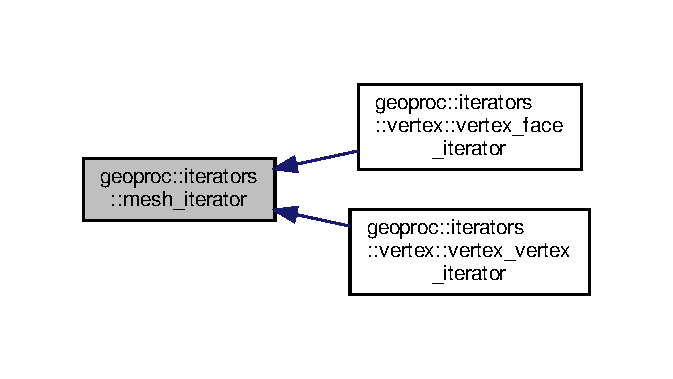
\includegraphics[width=323pt]{classgeoproc_1_1iterators_1_1mesh__iterator__inherit__graph}
\end{center}
\end{figure}


Collaboration diagram for geoproc\+:\+:iterators\+:\+:mesh\+\_\+iterator\+:\nopagebreak
\begin{figure}[H]
\begin{center}
\leavevmode
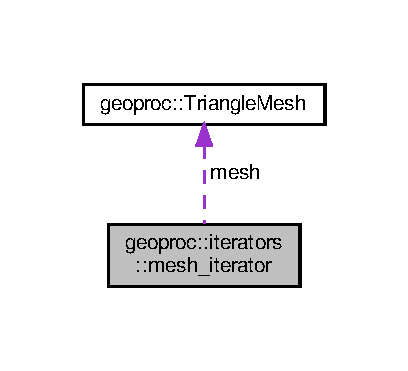
\includegraphics[width=196pt]{classgeoproc_1_1iterators_1_1mesh__iterator__coll__graph}
\end{center}
\end{figure}
\subsection*{Public Member Functions}
\begin{DoxyCompactItemize}
\item 
\hyperlink{classgeoproc_1_1iterators_1_1mesh__iterator_a785c3bccc57fd4db49de8aa89bc2d04e}{mesh\+\_\+iterator} (const \hyperlink{classgeoproc_1_1TriangleMesh}{Triangle\+Mesh} \&m)
\begin{DoxyCompactList}\small\item\em Default constructor. \end{DoxyCompactList}\item 
\mbox{\Hypertarget{classgeoproc_1_1iterators_1_1mesh__iterator_a240e308565715a31d4e721736e7ef9a7}\label{classgeoproc_1_1iterators_1_1mesh__iterator_a240e308565715a31d4e721736e7ef9a7}} 
virtual \hyperlink{classgeoproc_1_1iterators_1_1mesh__iterator_a240e308565715a31d4e721736e7ef9a7}{$\sim$mesh\+\_\+iterator} ()
\begin{DoxyCompactList}\small\item\em Destructor. \end{DoxyCompactList}\item 
\mbox{\Hypertarget{classgeoproc_1_1iterators_1_1mesh__iterator_a8a4d8b5c84941dd0a7cb7373abcd3fcc}\label{classgeoproc_1_1iterators_1_1mesh__iterator_a8a4d8b5c84941dd0a7cb7373abcd3fcc}} 
virtual int \hyperlink{classgeoproc_1_1iterators_1_1mesh__iterator_a8a4d8b5c84941dd0a7cb7373abcd3fcc}{init} (int idx)=0
\begin{DoxyCompactList}\small\item\em Initialise iterator with an index. \end{DoxyCompactList}\item 
\mbox{\Hypertarget{classgeoproc_1_1iterators_1_1mesh__iterator_ae6151b065602980d37a582977083ef42}\label{classgeoproc_1_1iterators_1_1mesh__iterator_ae6151b065602980d37a582977083ef42}} 
virtual int \hyperlink{classgeoproc_1_1iterators_1_1mesh__iterator_ae6151b065602980d37a582977083ef42}{current} () const =0
\begin{DoxyCompactList}\small\item\em Return index to current element. \end{DoxyCompactList}\item 
virtual int \hyperlink{classgeoproc_1_1iterators_1_1mesh__iterator_a32f1ddc2f83743a2b0a4633506601cfe}{next} ()=0
\begin{DoxyCompactList}\small\item\em Advances the iterator and returns the currently pointed element. \end{DoxyCompactList}\end{DoxyCompactItemize}
\subsection*{Protected Attributes}
\begin{DoxyCompactItemize}
\item 
\mbox{\Hypertarget{classgeoproc_1_1iterators_1_1mesh__iterator_a6102e0c43bcf7008597387a2f085ca0e}\label{classgeoproc_1_1iterators_1_1mesh__iterator_a6102e0c43bcf7008597387a2f085ca0e}} 
const \hyperlink{classgeoproc_1_1TriangleMesh}{Triangle\+Mesh} \& \hyperlink{classgeoproc_1_1iterators_1_1mesh__iterator_a6102e0c43bcf7008597387a2f085ca0e}{mesh}
\begin{DoxyCompactList}\small\item\em Constant reference to iterated mesh. \end{DoxyCompactList}\end{DoxyCompactItemize}


\subsection{Detailed Description}
Abstract iterator class. 

Defines three methods
\begin{DoxyItemize}
\item \hyperlink{classgeoproc_1_1iterators_1_1mesh__iterator_a8a4d8b5c84941dd0a7cb7373abcd3fcc}{init}
\item \hyperlink{classgeoproc_1_1iterators_1_1mesh__iterator_ae6151b065602980d37a582977083ef42}{current}
\item \hyperlink{classgeoproc_1_1iterators_1_1mesh__iterator_a32f1ddc2f83743a2b0a4633506601cfe}{next}
\end{DoxyItemize}

that have to be implemented in order to define the iteration on the mesh.

Each class that implements this one must document the behaviour of their implementations. 

\subsection{Constructor \& Destructor Documentation}
\mbox{\Hypertarget{classgeoproc_1_1iterators_1_1mesh__iterator_a785c3bccc57fd4db49de8aa89bc2d04e}\label{classgeoproc_1_1iterators_1_1mesh__iterator_a785c3bccc57fd4db49de8aa89bc2d04e}} 
\index{geoproc\+::iterators\+::mesh\+\_\+iterator@{geoproc\+::iterators\+::mesh\+\_\+iterator}!mesh\+\_\+iterator@{mesh\+\_\+iterator}}
\index{mesh\+\_\+iterator@{mesh\+\_\+iterator}!geoproc\+::iterators\+::mesh\+\_\+iterator@{geoproc\+::iterators\+::mesh\+\_\+iterator}}
\subsubsection{\texorpdfstring{mesh\+\_\+iterator()}{mesh\_iterator()}}
{\footnotesize\ttfamily geoproc\+::iterators\+::mesh\+\_\+iterator\+::mesh\+\_\+iterator (\begin{DoxyParamCaption}\item[{const \hyperlink{classgeoproc_1_1TriangleMesh}{Triangle\+Mesh} \&}]{m }\end{DoxyParamCaption})}



Default constructor. 


\begin{DoxyParams}{Parameters}
{\em m} & Constant reference to the iterated mesh. \\
\hline
\end{DoxyParams}
\begin{DoxyPrecond}{Precondition}
The mesh requires\+:
\begin{DoxyItemize}
\item Neighbourhood data (see \hyperlink{classgeoproc_1_1TriangleMesh_a84003dfdfd5e591c00f01a797578ff1f}{Triangle\+Mesh\+::make\+\_\+neighbourhood\+\_\+data}) 
\end{DoxyItemize}
\end{DoxyPrecond}


\subsection{Member Function Documentation}
\mbox{\Hypertarget{classgeoproc_1_1iterators_1_1mesh__iterator_a32f1ddc2f83743a2b0a4633506601cfe}\label{classgeoproc_1_1iterators_1_1mesh__iterator_a32f1ddc2f83743a2b0a4633506601cfe}} 
\index{geoproc\+::iterators\+::mesh\+\_\+iterator@{geoproc\+::iterators\+::mesh\+\_\+iterator}!next@{next}}
\index{next@{next}!geoproc\+::iterators\+::mesh\+\_\+iterator@{geoproc\+::iterators\+::mesh\+\_\+iterator}}
\subsubsection{\texorpdfstring{next()}{next()}}
{\footnotesize\ttfamily virtual int geoproc\+::iterators\+::mesh\+\_\+iterator\+::next (\begin{DoxyParamCaption}{ }\end{DoxyParamCaption})\hspace{0.3cm}{\ttfamily [pure virtual]}}



Advances the iterator and returns the currently pointed element. 

The iterator advances to a state in which it points to some element. The value returned is an index to that element. 

Implemented in \hyperlink{classgeoproc_1_1iterators_1_1vertex_1_1vertex__face__iterator_aa2a7fb3ee7e703d815e7f1664fbd99d4}{geoproc\+::iterators\+::vertex\+::vertex\+\_\+face\+\_\+iterator}, and \hyperlink{classgeoproc_1_1iterators_1_1vertex_1_1vertex__vertex__iterator_ad2041720a1d35892804c659de7b2dd44}{geoproc\+::iterators\+::vertex\+::vertex\+\_\+vertex\+\_\+iterator}.



The documentation for this class was generated from the following files\+:\begin{DoxyCompactItemize}
\item 
geoproc/iterators/mesh\+\_\+iterator.\+hpp\item 
geoproc/iterators/mesh\+\_\+iterator.\+cpp\end{DoxyCompactItemize}

\hypertarget{structgeoproc_1_1filter__frequencies_1_1smoothing__configuration}{}\section{geoproc\+:\+:filter\+\_\+frequencies\+:\+:smoothing\+\_\+configuration Struct Reference}
\label{structgeoproc_1_1filter__frequencies_1_1smoothing__configuration}\index{geoproc\+::filter\+\_\+frequencies\+::smoothing\+\_\+configuration@{geoproc\+::filter\+\_\+frequencies\+::smoothing\+\_\+configuration}}


A smoothing algorithm configuration.  




{\ttfamily \#include $<$band\+\_\+frequencies.\+hpp$>$}

\subsection*{Public Attributes}
\begin{DoxyCompactItemize}
\item 
\mbox{\Hypertarget{structgeoproc_1_1filter__frequencies_1_1smoothing__configuration_aa384c253639793b2230cb744444b97c2}\label{structgeoproc_1_1filter__frequencies_1_1smoothing__configuration_aa384c253639793b2230cb744444b97c2}} 
\hyperlink{namespacegeoproc_a396280579199558902594f4df72c01c7}{modifier} \hyperlink{structgeoproc_1_1filter__frequencies_1_1smoothing__configuration_aa384c253639793b2230cb744444b97c2}{so}
\begin{DoxyCompactList}\small\item\em Type of operator applied the algorithm uses. \end{DoxyCompactList}\item 
\mbox{\Hypertarget{structgeoproc_1_1filter__frequencies_1_1smoothing__configuration_a29f89d7b9df8ad82ed3759af569d8e67}\label{structgeoproc_1_1filter__frequencies_1_1smoothing__configuration_a29f89d7b9df8ad82ed3759af569d8e67}} 
\hyperlink{namespacegeoproc_a12e5a10581b53b9dd9a509127527f843}{weight} \hyperlink{structgeoproc_1_1filter__frequencies_1_1smoothing__configuration_a29f89d7b9df8ad82ed3759af569d8e67}{sw}
\begin{DoxyCompactList}\small\item\em Type of weight applied within the operator. \end{DoxyCompactList}\item 
\mbox{\Hypertarget{structgeoproc_1_1filter__frequencies_1_1smoothing__configuration_a801c2ab0af402978ec941776e1d20d00}\label{structgeoproc_1_1filter__frequencies_1_1smoothing__configuration_a801c2ab0af402978ec941776e1d20d00}} 
double \hyperlink{structgeoproc_1_1filter__frequencies_1_1smoothing__configuration_a801c2ab0af402978ec941776e1d20d00}{lambda}
\begin{DoxyCompactList}\small\item\em Value of parameter $\lambda$. \end{DoxyCompactList}\item 
\mbox{\Hypertarget{structgeoproc_1_1filter__frequencies_1_1smoothing__configuration_aa9f5a87ca7e0084e9ac6f3c40d30310c}\label{structgeoproc_1_1filter__frequencies_1_1smoothing__configuration_aa9f5a87ca7e0084e9ac6f3c40d30310c}} 
size\+\_\+t \hyperlink{structgeoproc_1_1filter__frequencies_1_1smoothing__configuration_aa9f5a87ca7e0084e9ac6f3c40d30310c}{n\+\_\+it}
\begin{DoxyCompactList}\small\item\em Amount of iterations of the algorithm. \end{DoxyCompactList}\end{DoxyCompactItemize}


\subsection{Detailed Description}
A smoothing algorithm configuration. 

Most smoothing algorithms require the same parameters. So, in order to easily configure the Band Frequencies obtention, this struct provides all the information necessary for it.

It contains,
\begin{DoxyItemize}
\item The operator used (see \hyperlink{structgeoproc_1_1filter__frequencies_1_1smoothing__configuration_aa384c253639793b2230cb744444b97c2}{so}).
\item The type of weight applied (see \hyperlink{structgeoproc_1_1filter__frequencies_1_1smoothing__configuration_a29f89d7b9df8ad82ed3759af569d8e67}{sw}).
\item Value of parameter $\lambda$ (see \hyperlink{structgeoproc_1_1filter__frequencies_1_1smoothing__configuration_a801c2ab0af402978ec941776e1d20d00}{lambda}).
\item Amount of iterations for the algorithm (see \hyperlink{structgeoproc_1_1filter__frequencies_1_1smoothing__configuration_aa9f5a87ca7e0084e9ac6f3c40d30310c}{n\+\_\+it}). 
\end{DoxyItemize}

The documentation for this struct was generated from the following file\+:\begin{DoxyCompactItemize}
\item 
geoproc/filter\+\_\+frequencies/band\+\_\+frequencies.\+hpp\end{DoxyCompactItemize}

\hypertarget{classgeoproc_1_1TriangleMesh}{}\section{geoproc\+:\+:Triangle\+Mesh Class Reference}
\label{classgeoproc_1_1TriangleMesh}\index{geoproc\+::\+Triangle\+Mesh@{geoproc\+::\+Triangle\+Mesh}}


Implementation of a triangular mesh.  




{\ttfamily \#include $<$triangle\+\_\+mesh.\+hpp$>$}

\subsection*{Public Member Functions}
\begin{DoxyCompactItemize}
\item 
\mbox{\Hypertarget{classgeoproc_1_1TriangleMesh_a73c49980eb81e2df75242515b5ef1ed7}\label{classgeoproc_1_1TriangleMesh_a73c49980eb81e2df75242515b5ef1ed7}} 
\hyperlink{classgeoproc_1_1TriangleMesh_a73c49980eb81e2df75242515b5ef1ed7}{Triangle\+Mesh} ()
\begin{DoxyCompactList}\small\item\em Default constructor. \end{DoxyCompactList}\item 
\mbox{\Hypertarget{classgeoproc_1_1TriangleMesh_ae660da7765a405ac44640d2ad46a6903}\label{classgeoproc_1_1TriangleMesh_ae660da7765a405ac44640d2ad46a6903}} 
\hyperlink{classgeoproc_1_1TriangleMesh_ae660da7765a405ac44640d2ad46a6903}{Triangle\+Mesh} (const \hyperlink{classgeoproc_1_1TriangleMesh}{Triangle\+Mesh} \&m)
\begin{DoxyCompactList}\small\item\em Copy constructor. \end{DoxyCompactList}\item 
\mbox{\Hypertarget{classgeoproc_1_1TriangleMesh_a587721dac1419702470fbca953fb7f1c}\label{classgeoproc_1_1TriangleMesh_a587721dac1419702470fbca953fb7f1c}} 
virtual \hyperlink{classgeoproc_1_1TriangleMesh_a587721dac1419702470fbca953fb7f1c}{$\sim$\+Triangle\+Mesh} ()
\begin{DoxyCompactList}\small\item\em Destructor. \end{DoxyCompactList}\item 
void \hyperlink{classgeoproc_1_1TriangleMesh_aa9ca26f1ededecd289d1a8800dca2c23}{set\+\_\+vertices} (const std\+::vector$<$ float $>$ \&coords)
\begin{DoxyCompactList}\small\item\em Sets the vertices to the mesh. \end{DoxyCompactList}\item 
void \hyperlink{classgeoproc_1_1TriangleMesh_a09b76789e908062501de253d360e0236}{set\+\_\+vertices} (const glm\+::vec3 $\ast$vs, int N)
\begin{DoxyCompactList}\small\item\em Sets the vertices to the mesh. \end{DoxyCompactList}\item 
void \hyperlink{classgeoproc_1_1TriangleMesh_a2bd9a343db1642d11b39b6fab5710d3a}{set\+\_\+vertices} (const std\+::vector$<$ glm\+::vec3 $>$ \&vs)
\begin{DoxyCompactList}\small\item\em Sets the vertices to the mesh. \end{DoxyCompactList}\item 
void \hyperlink{classgeoproc_1_1TriangleMesh_a5e35cad5c18195e6397f22bc951161f1}{set\+\_\+triangles} (const std\+::vector$<$ int $>$ \&tris)
\begin{DoxyCompactList}\small\item\em Adds the connectivity information to the mesh. \end{DoxyCompactList}\item 
void \hyperlink{classgeoproc_1_1TriangleMesh_a638f0267d7d8e51498330e414fa25bfe}{make\+\_\+normal\+\_\+vectors} ()
\begin{DoxyCompactList}\small\item\em Computes the normal of every triangle. \end{DoxyCompactList}\item 
void \hyperlink{classgeoproc_1_1TriangleMesh_a2b34ddfa21f906805451e6dbbb4ce064}{scale\+\_\+to\+\_\+unit} ()
\begin{DoxyCompactList}\small\item\em Reescales the mesh so that it fits in a unit box. \end{DoxyCompactList}\item 
void \hyperlink{classgeoproc_1_1TriangleMesh_a84003dfdfd5e591c00f01a797578ff1f}{make\+\_\+neighbourhood\+\_\+data} ()
\begin{DoxyCompactList}\small\item\em Builds the necessary tables to iterate through the one-\/ring of a vertex, .... \end{DoxyCompactList}\item 
void \hyperlink{classgeoproc_1_1TriangleMesh_a4657d7986fd9905c3a7b759e3d1b5442}{make\+\_\+angles\+\_\+area} ()
\begin{DoxyCompactList}\small\item\em Computes the angles and the areas of the triangles. \end{DoxyCompactList}\item 
void \hyperlink{classgeoproc_1_1TriangleMesh_ad11c9406e2677e4d72d53837206fd769}{make\+\_\+boundaries} ()
\begin{DoxyCompactList}\small\item\em Computes the boundaries of this mesh. \end{DoxyCompactList}\item 
void \hyperlink{classgeoproc_1_1TriangleMesh_abc27a4416e1d33b8718c4afb77a8acf5}{destroy} ()
\begin{DoxyCompactList}\small\item\em Frees all the memoery occupied by the mesh. \end{DoxyCompactList}\item 
\mbox{\Hypertarget{classgeoproc_1_1TriangleMesh_aa36cc7e86835794dcbbb3d823b4a39ac}\label{classgeoproc_1_1TriangleMesh_aa36cc7e86835794dcbbb3d823b4a39ac}} 
int \hyperlink{classgeoproc_1_1TriangleMesh_aa36cc7e86835794dcbbb3d823b4a39ac}{n\+\_\+vertices} () const
\begin{DoxyCompactList}\small\item\em Returns the number of vertices. \end{DoxyCompactList}\item 
\mbox{\Hypertarget{classgeoproc_1_1TriangleMesh_afdc430c1b3943895f85be7224b580ed6}\label{classgeoproc_1_1TriangleMesh_afdc430c1b3943895f85be7224b580ed6}} 
int \hyperlink{classgeoproc_1_1TriangleMesh_afdc430c1b3943895f85be7224b580ed6}{n\+\_\+edges} () const
\begin{DoxyCompactList}\small\item\em Returns the number of edges. \end{DoxyCompactList}\item 
\mbox{\Hypertarget{classgeoproc_1_1TriangleMesh_ac6db86ebd1e12d187f4bd4fcbb1e0809}\label{classgeoproc_1_1TriangleMesh_ac6db86ebd1e12d187f4bd4fcbb1e0809}} 
int \hyperlink{classgeoproc_1_1TriangleMesh_ac6db86ebd1e12d187f4bd4fcbb1e0809}{n\+\_\+triangles} () const
\begin{DoxyCompactList}\small\item\em Returns the number of triangles. \end{DoxyCompactList}\item 
\mbox{\Hypertarget{classgeoproc_1_1TriangleMesh_a6b8c186ba032170de9d4f36b4c1d298b}\label{classgeoproc_1_1TriangleMesh_a6b8c186ba032170de9d4f36b4c1d298b}} 
int \hyperlink{classgeoproc_1_1TriangleMesh_a6b8c186ba032170de9d4f36b4c1d298b}{n\+\_\+corners} () const
\begin{DoxyCompactList}\small\item\em Returns the number of corners. \end{DoxyCompactList}\item 
\mbox{\Hypertarget{classgeoproc_1_1TriangleMesh_a9986b64e0bb60968c95bdc9c3614959c}\label{classgeoproc_1_1TriangleMesh_a9986b64e0bb60968c95bdc9c3614959c}} 
int \hyperlink{classgeoproc_1_1TriangleMesh_a9986b64e0bb60968c95bdc9c3614959c}{n\+\_\+boundary\+\_\+edges} () const
\begin{DoxyCompactList}\small\item\em Returns the number of boundary edges. \end{DoxyCompactList}\item 
\mbox{\Hypertarget{classgeoproc_1_1TriangleMesh_a41a3d6325dcbd8891cd8cad06561b1b4}\label{classgeoproc_1_1TriangleMesh_a41a3d6325dcbd8891cd8cad06561b1b4}} 
size\+\_\+t \hyperlink{classgeoproc_1_1TriangleMesh_a41a3d6325dcbd8891cd8cad06561b1b4}{n\+\_\+boundaries} () const
\begin{DoxyCompactList}\small\item\em Returns the number of boundaries in this mesh. \end{DoxyCompactList}\item 
int \hyperlink{classgeoproc_1_1TriangleMesh_aba03ea01f69c0888e0aae17ec330d31d}{get\+\_\+vertex\+\_\+corner} (int c) const
\begin{DoxyCompactList}\small\item\em Returns the index of the vertex corresponding to corner {\itshape c}. \end{DoxyCompactList}\item 
int \hyperlink{classgeoproc_1_1TriangleMesh_a1a9e75bf79d26456527f943c653f31ab}{get\+\_\+corner\+\_\+vertex} (int v) const
\begin{DoxyCompactList}\small\item\em Returns a corner index for vertex {\itshape v}. \end{DoxyCompactList}\item 
int \hyperlink{classgeoproc_1_1TriangleMesh_acc3b8ff563eef67b3f55606a716d5dd9}{get\+\_\+edge\+\_\+vertex} (int v) const
\begin{DoxyCompactList}\small\item\em Returns the index of an edge incident to vertex {\itshape v}. \end{DoxyCompactList}\item 
int \hyperlink{classgeoproc_1_1TriangleMesh_a8f4d4fc9ea8c907d154605eee686807e}{get\+\_\+triangle\+\_\+corner} (int c) const
\begin{DoxyCompactList}\small\item\em Returns a triangle index for corner {\itshape c}. \end{DoxyCompactList}\item 
void \hyperlink{classgeoproc_1_1TriangleMesh_acd89c54ec14ddfb5d38f1baedb717fc2}{get\+\_\+corners\+\_\+triangle} (int t, int \&v0, int \&v1, int \&v2) const
\begin{DoxyCompactList}\small\item\em Returns the indexes of the vertices of a triangle. \end{DoxyCompactList}\item 
void \hyperlink{classgeoproc_1_1TriangleMesh_aab448f6f589f4c329b4daca635d9d865}{get\+\_\+vertices\+\_\+triangle} (int t, int \&v0, int \&v1, int \&v2) const
\begin{DoxyCompactList}\small\item\em Returns the indexes of the vertices of a triangle. \end{DoxyCompactList}\item 
void \hyperlink{classgeoproc_1_1TriangleMesh_af315fcda4f23dc0f3e9041e6d6d24601}{get\+\_\+vertices\+\_\+triangle} (int t, int v, int \&v0, int \&v1, int \&v2) const
\begin{DoxyCompactList}\small\item\em Returns the sorted indexes of the vertices of a face. \end{DoxyCompactList}\item 
int \hyperlink{classgeoproc_1_1TriangleMesh_a0ea38352c56a76d6def1fce67253f433}{get\+\_\+opposite\+\_\+corner} (int c) const
\begin{DoxyCompactList}\small\item\em Returns the corner opposite to corner c. \end{DoxyCompactList}\item 
const glm\+::vec3 \& \hyperlink{classgeoproc_1_1TriangleMesh_a9c231aaac3dfbfe9b6334df6cabb741e}{get\+\_\+vertex} (int v) const
\begin{DoxyCompactList}\small\item\em Returns the coordinates of a vertex. \end{DoxyCompactList}\item 
\mbox{\Hypertarget{classgeoproc_1_1TriangleMesh_a5dcfcb21cbd8e737813ff17cf5ecc566}\label{classgeoproc_1_1TriangleMesh_a5dcfcb21cbd8e737813ff17cf5ecc566}} 
const std\+::vector$<$ glm\+::vec3 $>$ \& \hyperlink{classgeoproc_1_1TriangleMesh_a5dcfcb21cbd8e737813ff17cf5ecc566}{get\+\_\+vertices} () const
\begin{DoxyCompactList}\small\item\em Returns a constant reference to all vertices of the mesh. \end{DoxyCompactList}\item 
\mbox{\Hypertarget{classgeoproc_1_1TriangleMesh_a5298c715723c9f247a998418d3fea286}\label{classgeoproc_1_1TriangleMesh_a5298c715723c9f247a998418d3fea286}} 
const glm\+::vec3 $\ast$ \hyperlink{classgeoproc_1_1TriangleMesh_a5298c715723c9f247a998418d3fea286}{get\+\_\+pvertices} () const
\begin{DoxyCompactList}\small\item\em Returns a constant reference to all vertices of the mesh. \end{DoxyCompactList}\item 
const std\+::vector$<$ glm\+::vec3 $>$ \& \hyperlink{classgeoproc_1_1TriangleMesh_ac21af48c99662a753251a5b7507c175f}{get\+\_\+normal\+\_\+vectors} () const
\begin{DoxyCompactList}\small\item\em Returns a constant reference to all normal vectors. \end{DoxyCompactList}\item 
float \hyperlink{classgeoproc_1_1TriangleMesh_ad43ef04d90bdde58951b3ee438b87c1e}{get\+\_\+triangle\+\_\+area} (int t) const
\begin{DoxyCompactList}\small\item\em Returns the area of face {\itshape f}. \end{DoxyCompactList}\item 
\mbox{\Hypertarget{classgeoproc_1_1TriangleMesh_a17b467002bd0f8373f7de367adfb1ec2}\label{classgeoproc_1_1TriangleMesh_a17b467002bd0f8373f7de367adfb1ec2}} 
const std\+::vector$<$ float $>$ \& \hyperlink{classgeoproc_1_1TriangleMesh_a17b467002bd0f8373f7de367adfb1ec2}{get\+\_\+areas} () const
\begin{DoxyCompactList}\small\item\em Returns the area of each triangle. \end{DoxyCompactList}\item 
const std\+::vector$<$ glm\+::vec3 $>$ \& \hyperlink{classgeoproc_1_1TriangleMesh_ae883c39c841c6598b0490224755f25b9}{get\+\_\+angles} () const
\begin{DoxyCompactList}\small\item\em Returns the angles on each triangle. \end{DoxyCompactList}\item 
\mbox{\Hypertarget{classgeoproc_1_1TriangleMesh_ad25eb7051e7eac604142d45929f33c19}\label{classgeoproc_1_1TriangleMesh_ad25eb7051e7eac604142d45929f33c19}} 
bool \hyperlink{classgeoproc_1_1TriangleMesh_ad25eb7051e7eac604142d45929f33c19}{are\+\_\+angles\+\_\+area\+\_\+valid} () const
\begin{DoxyCompactList}\small\item\em Is neighbourhood data valid? \end{DoxyCompactList}\item 
\mbox{\Hypertarget{classgeoproc_1_1TriangleMesh_aa6f95b95709a72a14a15638bfeeed3f9}\label{classgeoproc_1_1TriangleMesh_aa6f95b95709a72a14a15638bfeeed3f9}} 
bool \hyperlink{classgeoproc_1_1TriangleMesh_aa6f95b95709a72a14a15638bfeeed3f9}{is\+\_\+neighbourhood\+\_\+valid} () const
\begin{DoxyCompactList}\small\item\em Is neighbourhood data valid? \end{DoxyCompactList}\item 
\mbox{\Hypertarget{classgeoproc_1_1TriangleMesh_a409e399857e1a1abc9f23918ff5f5860}\label{classgeoproc_1_1TriangleMesh_a409e399857e1a1abc9f23918ff5f5860}} 
bool \hyperlink{classgeoproc_1_1TriangleMesh_a409e399857e1a1abc9f23918ff5f5860}{are\+\_\+boundaries\+\_\+valid} () const
\begin{DoxyCompactList}\small\item\em Are the boundaries valid? \end{DoxyCompactList}\item 
const std\+::vector$<$ int $>$ \& \hyperlink{classgeoproc_1_1TriangleMesh_ae73a760e61250eb2f474b8ab03a1e2ab}{get\+\_\+vertex\+\_\+edge} () const
\begin{DoxyCompactList}\small\item\em Returns a relation between vertices and edges. \end{DoxyCompactList}\item 
const std\+::vector$<$ int\mbox{[}3\mbox{]}$>$ \& \hyperlink{classgeoproc_1_1TriangleMesh_af56b3521a8df241f4f67c7f2bbacfa51}{get\+\_\+edges\+\_\+triangle} () const
\begin{DoxyCompactList}\small\item\em Returns a relation between tirnalges and edges. \end{DoxyCompactList}\item 
const std\+::vector$<$ \hyperlink{classgeoproc_1_1mesh__edge}{mesh\+\_\+edge} $>$ \& \hyperlink{classgeoproc_1_1TriangleMesh_a742e5769cb3e26303eb8ec1af57c9ac4}{get\+\_\+edges} () const
\begin{DoxyCompactList}\small\item\em Returns all edges in the mesh. \end{DoxyCompactList}\item 
const std\+::vector$<$ int $>$ \& \hyperlink{classgeoproc_1_1TriangleMesh_a0cf960fcf069954b51ce567304359d4e}{get\+\_\+boundary\+\_\+edges} () const
\begin{DoxyCompactList}\small\item\em Returns the boundary edges in this mesh. \end{DoxyCompactList}\item 
const std\+::vector$<$ std\+::vector$<$ int $>$ $>$ \& \hyperlink{classgeoproc_1_1TriangleMesh_a07a91ab963592c2560eec6409194ba66}{get\+\_\+boundaries} () const
\begin{DoxyCompactList}\small\item\em Returns the boundaries in this mesh. \end{DoxyCompactList}\item 
void \hyperlink{classgeoproc_1_1TriangleMesh_a00f918f8d96560f640efd244fd273cec}{get\+\_\+min\+\_\+max\+\_\+coordinates} (glm\+::vec3 \&m, glm\+::vec3 \&M) const
\begin{DoxyCompactList}\small\item\em Returns the minimum and maximum coordinates. \end{DoxyCompactList}\end{DoxyCompactItemize}
\subsection*{Protected Member Functions}
\begin{DoxyCompactItemize}
\item 
\mbox{\Hypertarget{classgeoproc_1_1TriangleMesh_aace37defd7566fed311222b7e22264a5}\label{classgeoproc_1_1TriangleMesh_aace37defd7566fed311222b7e22264a5}} 
void \hyperlink{classgeoproc_1_1TriangleMesh_aace37defd7566fed311222b7e22264a5}{invalidate\+\_\+areas\+\_\+angles} ()
\begin{DoxyCompactList}\small\item\em Sets to false the attribute \hyperlink{classgeoproc_1_1TriangleMesh_a046a6679ae404e02ae40d4d4d798b6f6}{angles\+\_\+area\+\_\+valid}. \end{DoxyCompactList}\item 
\mbox{\Hypertarget{classgeoproc_1_1TriangleMesh_add9ebc58773a0127b9a0467d33cfe3c6}\label{classgeoproc_1_1TriangleMesh_add9ebc58773a0127b9a0467d33cfe3c6}} 
void \hyperlink{classgeoproc_1_1TriangleMesh_add9ebc58773a0127b9a0467d33cfe3c6}{invalidate\+\_\+neighbourhood} ()
\begin{DoxyCompactList}\small\item\em Sets to false the attribute \hyperlink{classgeoproc_1_1TriangleMesh_a21205ec88e494f864db4d8247db70d3c}{neigh\+\_\+valid}. \end{DoxyCompactList}\item 
\mbox{\Hypertarget{classgeoproc_1_1TriangleMesh_af8c9c5ef993c961f24cdf189a990e6e8}\label{classgeoproc_1_1TriangleMesh_af8c9c5ef993c961f24cdf189a990e6e8}} 
void \hyperlink{classgeoproc_1_1TriangleMesh_af8c9c5ef993c961f24cdf189a990e6e8}{invalidate\+\_\+boundaries} ()
\begin{DoxyCompactList}\small\item\em Sets to false the attribute \hyperlink{classgeoproc_1_1TriangleMesh_a1384fa834aaa4ec3dc7c3b025b1ca528}{boundaries\+\_\+valid}. \end{DoxyCompactList}\item 
void \hyperlink{classgeoproc_1_1TriangleMesh_af83d7e4da9103a2d4ce965955b4520f7}{invalidate\+\_\+state} ()
\begin{DoxyCompactList}\small\item\em Invalidates the whole state of the mesh. \end{DoxyCompactList}\item 
void \hyperlink{classgeoproc_1_1TriangleMesh_a1680c786572ac504621f253b7407d4f7}{copy\+\_\+mesh} (const \hyperlink{classgeoproc_1_1TriangleMesh}{Triangle\+Mesh} \&m)
\begin{DoxyCompactList}\small\item\em Copies mesh {\itshape m} contents into this one. \end{DoxyCompactList}\item 
float \hyperlink{classgeoproc_1_1TriangleMesh_a8a07f19f9d81952752d9c8973a2eb011}{get\+\_\+triangle\+\_\+area} (int i, int j, int k) const
\begin{DoxyCompactList}\small\item\em Assuming the vertices make a triangle, return its area. \end{DoxyCompactList}\end{DoxyCompactItemize}
\subsection*{Protected Attributes}
\begin{DoxyCompactItemize}
\item 
\mbox{\Hypertarget{classgeoproc_1_1TriangleMesh_a82c3351de37daa9440f53597f080992d}\label{classgeoproc_1_1TriangleMesh_a82c3351de37daa9440f53597f080992d}} 
std\+::vector$<$ glm\+::vec3 $>$ \hyperlink{classgeoproc_1_1TriangleMesh_a82c3351de37daa9440f53597f080992d}{vertices}
\begin{DoxyCompactList}\small\item\em The set of vertices of the mesh. \end{DoxyCompactList}\item 
std\+::vector$<$ int $>$ \hyperlink{classgeoproc_1_1TriangleMesh_ad1cf20622f2bb080100862f413bd89c2}{triangles}
\begin{DoxyCompactList}\small\item\em The set of triangles of the mesh. \end{DoxyCompactList}\item 
std\+::vector$<$ glm\+::vec3 $>$ \hyperlink{classgeoproc_1_1TriangleMesh_ab9030a0301b2fe5868ad6c08692cce09}{normal\+\_\+vectors}
\begin{DoxyCompactList}\small\item\em Normal vector for every triangle of the mesh. \end{DoxyCompactList}\item 
std\+::vector$<$ glm\+::vec3 $>$ \hyperlink{classgeoproc_1_1TriangleMesh_ab255af87d20d76ad84246560fa3579b3}{angles}
\begin{DoxyCompactList}\small\item\em Angles of each triangle. \end{DoxyCompactList}\item 
std\+::vector$<$ float $>$ \hyperlink{classgeoproc_1_1TriangleMesh_a684ecaaa03f1739856bba03167e51dd1}{areas}
\begin{DoxyCompactList}\small\item\em Area of each triangle. \end{DoxyCompactList}\item 
std\+::vector$<$ int $>$ \hyperlink{classgeoproc_1_1TriangleMesh_a2604795c90c694116513252b86d242b4}{opposite\+\_\+corners}
\begin{DoxyCompactList}\small\item\em The set of opposite corners. \end{DoxyCompactList}\item 
std\+::vector$<$ int $>$ \hyperlink{classgeoproc_1_1TriangleMesh_ab9610d614e081deb28010d237fecd55b}{corners}
\begin{DoxyCompactList}\small\item\em Corner table. \end{DoxyCompactList}\item 
std\+::vector$<$ \hyperlink{classgeoproc_1_1mesh__edge}{mesh\+\_\+edge} $>$ \hyperlink{classgeoproc_1_1TriangleMesh_ab10f052ad932cd78056a55b58ddd475c}{all\+\_\+edges}
\begin{DoxyCompactList}\small\item\em Edges of this mesh. \end{DoxyCompactList}\item 
std\+::vector$<$ int\mbox{[}3\mbox{]}$>$ \hyperlink{classgeoproc_1_1TriangleMesh_ad72cdd2358e815a09c07176730b4e0a5}{edges\+\_\+per\+\_\+triangle}
\begin{DoxyCompactList}\small\item\em Edges per triangle. \end{DoxyCompactList}\item 
std\+::vector$<$ int $>$ \hyperlink{classgeoproc_1_1TriangleMesh_abbc25699f67776fc99c909124b0c584a}{vertex\+\_\+edge}
\begin{DoxyCompactList}\small\item\em Edge index for each vertex. \end{DoxyCompactList}\item 
std\+::vector$<$ int $>$ \hyperlink{classgeoproc_1_1TriangleMesh_a142a764ddf07b98c7efcd596d88c3f87}{boundary\+\_\+edges}
\begin{DoxyCompactList}\small\item\em Boundary edges of the mesh. \end{DoxyCompactList}\item 
std\+::vector$<$ std\+::vector$<$ int $>$ $>$ \hyperlink{classgeoproc_1_1TriangleMesh_a57162eac37831c87786a8dab8331d72f}{boundaries}
\begin{DoxyCompactList}\small\item\em Boundaries of this mesh. \end{DoxyCompactList}\item 
\mbox{\Hypertarget{classgeoproc_1_1TriangleMesh_aab5e7d8baf6f6cd7b5655b4c89f79e00}\label{classgeoproc_1_1TriangleMesh_aab5e7d8baf6f6cd7b5655b4c89f79e00}} 
glm\+::vec3 \hyperlink{classgeoproc_1_1TriangleMesh_aab5e7d8baf6f6cd7b5655b4c89f79e00}{min\+\_\+coord}
\begin{DoxyCompactList}\small\item\em Minimum value of x-\/,y-\/, and z-\/coordinates. \end{DoxyCompactList}\item 
\mbox{\Hypertarget{classgeoproc_1_1TriangleMesh_acffb17b164f0428aa01316b0a08bc2a3}\label{classgeoproc_1_1TriangleMesh_acffb17b164f0428aa01316b0a08bc2a3}} 
glm\+::vec3 \hyperlink{classgeoproc_1_1TriangleMesh_acffb17b164f0428aa01316b0a08bc2a3}{max\+\_\+coord}
\begin{DoxyCompactList}\small\item\em Maximum value of x-\/,y-\/, and z-\/coordinates. \end{DoxyCompactList}\item 
\mbox{\Hypertarget{classgeoproc_1_1TriangleMesh_a046a6679ae404e02ae40d4d4d798b6f6}\label{classgeoproc_1_1TriangleMesh_a046a6679ae404e02ae40d4d4d798b6f6}} 
bool \hyperlink{classgeoproc_1_1TriangleMesh_a046a6679ae404e02ae40d4d4d798b6f6}{angles\+\_\+area\+\_\+valid}
\begin{DoxyCompactList}\small\item\em Are the computed triangle angles and areas valid? \end{DoxyCompactList}\item 
bool \hyperlink{classgeoproc_1_1TriangleMesh_a21205ec88e494f864db4d8247db70d3c}{neigh\+\_\+valid}
\begin{DoxyCompactList}\small\item\em Is the neighbourhood data valid? \end{DoxyCompactList}\item 
bool \hyperlink{classgeoproc_1_1TriangleMesh_a1384fa834aaa4ec3dc7c3b025b1ca528}{boundaries\+\_\+valid}
\begin{DoxyCompactList}\small\item\em Are the boundaries of the mesh valid? \end{DoxyCompactList}\end{DoxyCompactItemize}


\subsection{Detailed Description}
Implementation of a triangular mesh. 

It contains the vertices of a triangular mesh (\hyperlink{classgeoproc_1_1TriangleMesh_a82c3351de37daa9440f53597f080992d}{vertices}) which are related using indices (\hyperlink{classgeoproc_1_1TriangleMesh_ad1cf20622f2bb080100862f413bd89c2}{triangles}), hence following the usual implementation.

It also stores normal vectors per triangle (\hyperlink{classgeoproc_1_1TriangleMesh_ab9030a0301b2fe5868ad6c08692cce09}{normal\+\_\+vectors}), angles and area of each triangle (\hyperlink{classgeoproc_1_1TriangleMesh_ab255af87d20d76ad84246560fa3579b3}{angles}, \hyperlink{classgeoproc_1_1TriangleMesh_a684ecaaa03f1739856bba03167e51dd1}{areas}), and implements the corner table data structure (see \hyperlink{classgeoproc_1_1TriangleMesh_ab9610d614e081deb28010d237fecd55b}{corners}, \hyperlink{classgeoproc_1_1TriangleMesh_a2604795c90c694116513252b86d242b4}{opposite\+\_\+corners}).

Finally, it holds other interesting information about the structure of the mesh, like boundaries (see \hyperlink{classgeoproc_1_1TriangleMesh_a142a764ddf07b98c7efcd596d88c3f87}{boundary\+\_\+edges}, \hyperlink{classgeoproc_1_1TriangleMesh_a57162eac37831c87786a8dab8331d72f}{boundaries}). 

\subsection{Member Function Documentation}
\mbox{\Hypertarget{classgeoproc_1_1TriangleMesh_a1680c786572ac504621f253b7407d4f7}\label{classgeoproc_1_1TriangleMesh_a1680c786572ac504621f253b7407d4f7}} 
\index{geoproc\+::\+Triangle\+Mesh@{geoproc\+::\+Triangle\+Mesh}!copy\+\_\+mesh@{copy\+\_\+mesh}}
\index{copy\+\_\+mesh@{copy\+\_\+mesh}!geoproc\+::\+Triangle\+Mesh@{geoproc\+::\+Triangle\+Mesh}}
\subsubsection{\texorpdfstring{copy\+\_\+mesh()}{copy\_mesh()}}
{\footnotesize\ttfamily void geoproc\+::\+Triangle\+Mesh\+::copy\+\_\+mesh (\begin{DoxyParamCaption}\item[{const \hyperlink{classgeoproc_1_1TriangleMesh}{Triangle\+Mesh} \&}]{m }\end{DoxyParamCaption})\hspace{0.3cm}{\ttfamily [protected]}}



Copies mesh {\itshape m} contents into this one. 

This mesh is previously freed. 
\begin{DoxyParams}{Parameters}
{\em m} & Mesh to be copied. \\
\hline
\end{DoxyParams}
\mbox{\Hypertarget{classgeoproc_1_1TriangleMesh_abc27a4416e1d33b8718c4afb77a8acf5}\label{classgeoproc_1_1TriangleMesh_abc27a4416e1d33b8718c4afb77a8acf5}} 
\index{geoproc\+::\+Triangle\+Mesh@{geoproc\+::\+Triangle\+Mesh}!destroy@{destroy}}
\index{destroy@{destroy}!geoproc\+::\+Triangle\+Mesh@{geoproc\+::\+Triangle\+Mesh}}
\subsubsection{\texorpdfstring{destroy()}{destroy()}}
{\footnotesize\ttfamily void geoproc\+::\+Triangle\+Mesh\+::destroy (\begin{DoxyParamCaption}{ }\end{DoxyParamCaption})}



Frees all the memoery occupied by the mesh. 

Clears the contents of\+:
\begin{DoxyItemize}
\item \hyperlink{classgeoproc_1_1TriangleMesh_a82c3351de37daa9440f53597f080992d}{vertices},
\item \hyperlink{classgeoproc_1_1TriangleMesh_ad1cf20622f2bb080100862f413bd89c2}{triangles},
\item \hyperlink{classgeoproc_1_1TriangleMesh_ab9030a0301b2fe5868ad6c08692cce09}{normal\+\_\+vectors},
\item \hyperlink{classgeoproc_1_1TriangleMesh_ab255af87d20d76ad84246560fa3579b3}{angles},
\item \hyperlink{classgeoproc_1_1TriangleMesh_a684ecaaa03f1739856bba03167e51dd1}{areas},
\item \hyperlink{classgeoproc_1_1TriangleMesh_a2604795c90c694116513252b86d242b4}{opposite\+\_\+corners},
\item \hyperlink{classgeoproc_1_1TriangleMesh_ab9610d614e081deb28010d237fecd55b}{corners},
\item \hyperlink{classgeoproc_1_1TriangleMesh_a142a764ddf07b98c7efcd596d88c3f87}{boundary\+\_\+edges},
\item \hyperlink{classgeoproc_1_1TriangleMesh_a57162eac37831c87786a8dab8331d72f}{boundaries},
\item \hyperlink{classgeoproc_1_1TriangleMesh_ab10f052ad932cd78056a55b58ddd475c}{all\+\_\+edges},
\item \hyperlink{classgeoproc_1_1TriangleMesh_abbc25699f67776fc99c909124b0c584a}{vertex\+\_\+edge} 
\end{DoxyItemize}\mbox{\Hypertarget{classgeoproc_1_1TriangleMesh_ae883c39c841c6598b0490224755f25b9}\label{classgeoproc_1_1TriangleMesh_ae883c39c841c6598b0490224755f25b9}} 
\index{geoproc\+::\+Triangle\+Mesh@{geoproc\+::\+Triangle\+Mesh}!get\+\_\+angles@{get\+\_\+angles}}
\index{get\+\_\+angles@{get\+\_\+angles}!geoproc\+::\+Triangle\+Mesh@{geoproc\+::\+Triangle\+Mesh}}
\subsubsection{\texorpdfstring{get\+\_\+angles()}{get\_angles()}}
{\footnotesize\ttfamily const vector$<$ vec3 $>$ \& geoproc\+::\+Triangle\+Mesh\+::get\+\_\+angles (\begin{DoxyParamCaption}{ }\end{DoxyParamCaption}) const}



Returns the angles on each triangle. 

\begin{DoxyPrecond}{Precondition}
Angles and area data must be valid 
\end{DoxyPrecond}
\mbox{\Hypertarget{classgeoproc_1_1TriangleMesh_a07a91ab963592c2560eec6409194ba66}\label{classgeoproc_1_1TriangleMesh_a07a91ab963592c2560eec6409194ba66}} 
\index{geoproc\+::\+Triangle\+Mesh@{geoproc\+::\+Triangle\+Mesh}!get\+\_\+boundaries@{get\+\_\+boundaries}}
\index{get\+\_\+boundaries@{get\+\_\+boundaries}!geoproc\+::\+Triangle\+Mesh@{geoproc\+::\+Triangle\+Mesh}}
\subsubsection{\texorpdfstring{get\+\_\+boundaries()}{get\_boundaries()}}
{\footnotesize\ttfamily const vector$<$ vector$<$ int $>$ $>$ \& geoproc\+::\+Triangle\+Mesh\+::get\+\_\+boundaries (\begin{DoxyParamCaption}{ }\end{DoxyParamCaption}) const}



Returns the boundaries in this mesh. 

\begin{DoxyPrecond}{Precondition}
Boundaries have to be valid (\hyperlink{classgeoproc_1_1TriangleMesh_a409e399857e1a1abc9f23918ff5f5860}{are\+\_\+boundaries\+\_\+valid()} evaluates to true). 
\end{DoxyPrecond}
\mbox{\Hypertarget{classgeoproc_1_1TriangleMesh_a0cf960fcf069954b51ce567304359d4e}\label{classgeoproc_1_1TriangleMesh_a0cf960fcf069954b51ce567304359d4e}} 
\index{geoproc\+::\+Triangle\+Mesh@{geoproc\+::\+Triangle\+Mesh}!get\+\_\+boundary\+\_\+edges@{get\+\_\+boundary\+\_\+edges}}
\index{get\+\_\+boundary\+\_\+edges@{get\+\_\+boundary\+\_\+edges}!geoproc\+::\+Triangle\+Mesh@{geoproc\+::\+Triangle\+Mesh}}
\subsubsection{\texorpdfstring{get\+\_\+boundary\+\_\+edges()}{get\_boundary\_edges()}}
{\footnotesize\ttfamily const vector$<$ int $>$ \& geoproc\+::\+Triangle\+Mesh\+::get\+\_\+boundary\+\_\+edges (\begin{DoxyParamCaption}{ }\end{DoxyParamCaption}) const}



Returns the boundary edges in this mesh. 

\begin{DoxyPrecond}{Precondition}
Boundaries have to be valid (\hyperlink{classgeoproc_1_1TriangleMesh_a409e399857e1a1abc9f23918ff5f5860}{are\+\_\+boundaries\+\_\+valid()} evaluates to true). 
\end{DoxyPrecond}
\mbox{\Hypertarget{classgeoproc_1_1TriangleMesh_a1a9e75bf79d26456527f943c653f31ab}\label{classgeoproc_1_1TriangleMesh_a1a9e75bf79d26456527f943c653f31ab}} 
\index{geoproc\+::\+Triangle\+Mesh@{geoproc\+::\+Triangle\+Mesh}!get\+\_\+corner\+\_\+vertex@{get\+\_\+corner\+\_\+vertex}}
\index{get\+\_\+corner\+\_\+vertex@{get\+\_\+corner\+\_\+vertex}!geoproc\+::\+Triangle\+Mesh@{geoproc\+::\+Triangle\+Mesh}}
\subsubsection{\texorpdfstring{get\+\_\+corner\+\_\+vertex()}{get\_corner\_vertex()}}
{\footnotesize\ttfamily int geoproc\+::\+Triangle\+Mesh\+::get\+\_\+corner\+\_\+vertex (\begin{DoxyParamCaption}\item[{int}]{v }\end{DoxyParamCaption}) const}



Returns a corner index for vertex {\itshape v}. 


\begin{DoxyParams}{Parameters}
{\em v} & A valid vertex index\+: 0 $<$= {\itshape v} $<$ number of vertices. \\
\hline
\end{DoxyParams}
\begin{DoxyPrecond}{Precondition}
Neighbourhood data must be valid, i.\+e, the result of \hyperlink{classgeoproc_1_1TriangleMesh_aa6f95b95709a72a14a15638bfeeed3f9}{is\+\_\+neighbourhood\+\_\+valid()} must be true. If false, call \hyperlink{classgeoproc_1_1TriangleMesh_a84003dfdfd5e591c00f01a797578ff1f}{make\+\_\+neighbourhood\+\_\+data}. 
\end{DoxyPrecond}
\begin{DoxyReturn}{Returns}
Returns a valid corner index (unless there are no faces in this mesh). Returns {\itshape c} such that 0 $<$= {\itshape c} $<$ number of triangles 
\end{DoxyReturn}
\mbox{\Hypertarget{classgeoproc_1_1TriangleMesh_acd89c54ec14ddfb5d38f1baedb717fc2}\label{classgeoproc_1_1TriangleMesh_acd89c54ec14ddfb5d38f1baedb717fc2}} 
\index{geoproc\+::\+Triangle\+Mesh@{geoproc\+::\+Triangle\+Mesh}!get\+\_\+corners\+\_\+triangle@{get\+\_\+corners\+\_\+triangle}}
\index{get\+\_\+corners\+\_\+triangle@{get\+\_\+corners\+\_\+triangle}!geoproc\+::\+Triangle\+Mesh@{geoproc\+::\+Triangle\+Mesh}}
\subsubsection{\texorpdfstring{get\+\_\+corners\+\_\+triangle()}{get\_corners\_triangle()}}
{\footnotesize\ttfamily void geoproc\+::\+Triangle\+Mesh\+::get\+\_\+corners\+\_\+triangle (\begin{DoxyParamCaption}\item[{int}]{t,  }\item[{int \&}]{v0,  }\item[{int \&}]{v1,  }\item[{int \&}]{v2 }\end{DoxyParamCaption}) const}



Returns the indexes of the vertices of a triangle. 

It is guaranteed that the order of the vertices is the same as it is given in the loaded file. 
\begin{DoxyParams}[1]{Parameters}
 & {\em t} & A valid triangle index\+: 0 $<$= {\itshape t} $<$ number of triangles. \\
\hline
\mbox{\tt out}  & {\em v0} & The first vertex index of the face. \\
\hline
\mbox{\tt out}  & {\em v1} & The second vertex index of the face. \\
\hline
\mbox{\tt out}  & {\em v2} & The third vertex index of the face. \\
\hline
\end{DoxyParams}
\mbox{\Hypertarget{classgeoproc_1_1TriangleMesh_acc3b8ff563eef67b3f55606a716d5dd9}\label{classgeoproc_1_1TriangleMesh_acc3b8ff563eef67b3f55606a716d5dd9}} 
\index{geoproc\+::\+Triangle\+Mesh@{geoproc\+::\+Triangle\+Mesh}!get\+\_\+edge\+\_\+vertex@{get\+\_\+edge\+\_\+vertex}}
\index{get\+\_\+edge\+\_\+vertex@{get\+\_\+edge\+\_\+vertex}!geoproc\+::\+Triangle\+Mesh@{geoproc\+::\+Triangle\+Mesh}}
\subsubsection{\texorpdfstring{get\+\_\+edge\+\_\+vertex()}{get\_edge\_vertex()}}
{\footnotesize\ttfamily int geoproc\+::\+Triangle\+Mesh\+::get\+\_\+edge\+\_\+vertex (\begin{DoxyParamCaption}\item[{int}]{v }\end{DoxyParamCaption}) const}



Returns the index of an edge incident to vertex {\itshape v}. 


\begin{DoxyParams}{Parameters}
{\em v} & A valid vertex index\+: 0 $<$= {\itshape v} $<$ number of vertices. \\
\hline
\end{DoxyParams}
\begin{DoxyPrecond}{Precondition}
Neighbourhood data must be valid, i.\+e, the result of \hyperlink{classgeoproc_1_1TriangleMesh_aa6f95b95709a72a14a15638bfeeed3f9}{is\+\_\+neighbourhood\+\_\+valid()} must be true. If false, call \hyperlink{classgeoproc_1_1TriangleMesh_a84003dfdfd5e591c00f01a797578ff1f}{make\+\_\+neighbourhood\+\_\+data}. 
\end{DoxyPrecond}
\begin{DoxyReturn}{Returns}
Returns a valid edge index. 
\end{DoxyReturn}
\mbox{\Hypertarget{classgeoproc_1_1TriangleMesh_a742e5769cb3e26303eb8ec1af57c9ac4}\label{classgeoproc_1_1TriangleMesh_a742e5769cb3e26303eb8ec1af57c9ac4}} 
\index{geoproc\+::\+Triangle\+Mesh@{geoproc\+::\+Triangle\+Mesh}!get\+\_\+edges@{get\+\_\+edges}}
\index{get\+\_\+edges@{get\+\_\+edges}!geoproc\+::\+Triangle\+Mesh@{geoproc\+::\+Triangle\+Mesh}}
\subsubsection{\texorpdfstring{get\+\_\+edges()}{get\_edges()}}
{\footnotesize\ttfamily const vector$<$ \hyperlink{classgeoproc_1_1mesh__edge}{mesh\+\_\+edge} $>$ \& geoproc\+::\+Triangle\+Mesh\+::get\+\_\+edges (\begin{DoxyParamCaption}{ }\end{DoxyParamCaption}) const}



Returns all edges in the mesh. 

\begin{DoxyPrecond}{Precondition}
Neighbourhood has to be valid (\hyperlink{classgeoproc_1_1TriangleMesh_aa6f95b95709a72a14a15638bfeeed3f9}{is\+\_\+neighbourhood\+\_\+valid()} evaluates to true). 
\end{DoxyPrecond}
\mbox{\Hypertarget{classgeoproc_1_1TriangleMesh_af56b3521a8df241f4f67c7f2bbacfa51}\label{classgeoproc_1_1TriangleMesh_af56b3521a8df241f4f67c7f2bbacfa51}} 
\index{geoproc\+::\+Triangle\+Mesh@{geoproc\+::\+Triangle\+Mesh}!get\+\_\+edges\+\_\+triangle@{get\+\_\+edges\+\_\+triangle}}
\index{get\+\_\+edges\+\_\+triangle@{get\+\_\+edges\+\_\+triangle}!geoproc\+::\+Triangle\+Mesh@{geoproc\+::\+Triangle\+Mesh}}
\subsubsection{\texorpdfstring{get\+\_\+edges\+\_\+triangle()}{get\_edges\_triangle()}}
{\footnotesize\ttfamily const vector$<$ int\mbox{[}3\mbox{]}$>$ \& geoproc\+::\+Triangle\+Mesh\+::get\+\_\+edges\+\_\+triangle (\begin{DoxyParamCaption}{ }\end{DoxyParamCaption}) const}



Returns a relation between tirnalges and edges. 

\begin{DoxyPrecond}{Precondition}
Neighbourhood has to be valid (\hyperlink{classgeoproc_1_1TriangleMesh_aa6f95b95709a72a14a15638bfeeed3f9}{is\+\_\+neighbourhood\+\_\+valid()} evaluates to true). 
\end{DoxyPrecond}
\mbox{\Hypertarget{classgeoproc_1_1TriangleMesh_a00f918f8d96560f640efd244fd273cec}\label{classgeoproc_1_1TriangleMesh_a00f918f8d96560f640efd244fd273cec}} 
\index{geoproc\+::\+Triangle\+Mesh@{geoproc\+::\+Triangle\+Mesh}!get\+\_\+min\+\_\+max\+\_\+coordinates@{get\+\_\+min\+\_\+max\+\_\+coordinates}}
\index{get\+\_\+min\+\_\+max\+\_\+coordinates@{get\+\_\+min\+\_\+max\+\_\+coordinates}!geoproc\+::\+Triangle\+Mesh@{geoproc\+::\+Triangle\+Mesh}}
\subsubsection{\texorpdfstring{get\+\_\+min\+\_\+max\+\_\+coordinates()}{get\_min\_max\_coordinates()}}
{\footnotesize\ttfamily void geoproc\+::\+Triangle\+Mesh\+::get\+\_\+min\+\_\+max\+\_\+coordinates (\begin{DoxyParamCaption}\item[{glm\+::vec3 \&}]{m,  }\item[{glm\+::vec3 \&}]{M }\end{DoxyParamCaption}) const}



Returns the minimum and maximum coordinates. 


\begin{DoxyParams}[1]{Parameters}
\mbox{\tt out}  & {\em m} & Minimum x-\/,y-\/,z-\/ coordinates. \\
\hline
\mbox{\tt out}  & {\em M} & Maximum x-\/,y-\/,z-\/ coordinates. \\
\hline
\end{DoxyParams}
\mbox{\Hypertarget{classgeoproc_1_1TriangleMesh_ac21af48c99662a753251a5b7507c175f}\label{classgeoproc_1_1TriangleMesh_ac21af48c99662a753251a5b7507c175f}} 
\index{geoproc\+::\+Triangle\+Mesh@{geoproc\+::\+Triangle\+Mesh}!get\+\_\+normal\+\_\+vectors@{get\+\_\+normal\+\_\+vectors}}
\index{get\+\_\+normal\+\_\+vectors@{get\+\_\+normal\+\_\+vectors}!geoproc\+::\+Triangle\+Mesh@{geoproc\+::\+Triangle\+Mesh}}
\subsubsection{\texorpdfstring{get\+\_\+normal\+\_\+vectors()}{get\_normal\_vectors()}}
{\footnotesize\ttfamily const vector$<$ vec3 $>$ \& geoproc\+::\+Triangle\+Mesh\+::get\+\_\+normal\+\_\+vectors (\begin{DoxyParamCaption}{ }\end{DoxyParamCaption}) const}



Returns a constant reference to all normal vectors. 

\begin{DoxyReturn}{Returns}
Returns a constant reference to \hyperlink{classgeoproc_1_1TriangleMesh_ab9030a0301b2fe5868ad6c08692cce09}{normal\+\_\+vectors}. 
\end{DoxyReturn}
\mbox{\Hypertarget{classgeoproc_1_1TriangleMesh_a0ea38352c56a76d6def1fce67253f433}\label{classgeoproc_1_1TriangleMesh_a0ea38352c56a76d6def1fce67253f433}} 
\index{geoproc\+::\+Triangle\+Mesh@{geoproc\+::\+Triangle\+Mesh}!get\+\_\+opposite\+\_\+corner@{get\+\_\+opposite\+\_\+corner}}
\index{get\+\_\+opposite\+\_\+corner@{get\+\_\+opposite\+\_\+corner}!geoproc\+::\+Triangle\+Mesh@{geoproc\+::\+Triangle\+Mesh}}
\subsubsection{\texorpdfstring{get\+\_\+opposite\+\_\+corner()}{get\_opposite\_corner()}}
{\footnotesize\ttfamily int geoproc\+::\+Triangle\+Mesh\+::get\+\_\+opposite\+\_\+corner (\begin{DoxyParamCaption}\item[{int}]{c }\end{DoxyParamCaption}) const}



Returns the corner opposite to corner c. 


\begin{DoxyParams}{Parameters}
{\em c} & Valid corner index\+: 0 $<$= {\itshape c} $<$ number of corners. \\
\hline
\end{DoxyParams}
\begin{DoxyPrecond}{Precondition}
Neighbourhood data must be valid, i.\+e, the result of \hyperlink{classgeoproc_1_1TriangleMesh_aa6f95b95709a72a14a15638bfeeed3f9}{is\+\_\+neighbourhood\+\_\+valid()} must be true. If false, call \hyperlink{classgeoproc_1_1TriangleMesh_a84003dfdfd5e591c00f01a797578ff1f}{make\+\_\+neighbourhood\+\_\+data}. 
\end{DoxyPrecond}
\begin{DoxyReturn}{Returns}
Returns -\/1 if there is no opposite corner (the case of hard boundary). Returns a valid corner index otherwise. 
\end{DoxyReturn}
\mbox{\Hypertarget{classgeoproc_1_1TriangleMesh_a8a07f19f9d81952752d9c8973a2eb011}\label{classgeoproc_1_1TriangleMesh_a8a07f19f9d81952752d9c8973a2eb011}} 
\index{geoproc\+::\+Triangle\+Mesh@{geoproc\+::\+Triangle\+Mesh}!get\+\_\+triangle\+\_\+area@{get\+\_\+triangle\+\_\+area}}
\index{get\+\_\+triangle\+\_\+area@{get\+\_\+triangle\+\_\+area}!geoproc\+::\+Triangle\+Mesh@{geoproc\+::\+Triangle\+Mesh}}
\subsubsection{\texorpdfstring{get\+\_\+triangle\+\_\+area()}{get\_triangle\_area()}\hspace{0.1cm}{\footnotesize\ttfamily [1/2]}}
{\footnotesize\ttfamily float geoproc\+::\+Triangle\+Mesh\+::get\+\_\+triangle\+\_\+area (\begin{DoxyParamCaption}\item[{int}]{i,  }\item[{int}]{j,  }\item[{int}]{k }\end{DoxyParamCaption}) const\hspace{0.3cm}{\ttfamily [protected]}}



Assuming the vertices make a triangle, return its area. 


\begin{DoxyParams}{Parameters}
{\em i} & A valid vertex index. \\
\hline
{\em j} & A valid vertex index. \\
\hline
{\em k} & A valid vertex index. \\
\hline
\end{DoxyParams}
\mbox{\Hypertarget{classgeoproc_1_1TriangleMesh_ad43ef04d90bdde58951b3ee438b87c1e}\label{classgeoproc_1_1TriangleMesh_ad43ef04d90bdde58951b3ee438b87c1e}} 
\index{geoproc\+::\+Triangle\+Mesh@{geoproc\+::\+Triangle\+Mesh}!get\+\_\+triangle\+\_\+area@{get\+\_\+triangle\+\_\+area}}
\index{get\+\_\+triangle\+\_\+area@{get\+\_\+triangle\+\_\+area}!geoproc\+::\+Triangle\+Mesh@{geoproc\+::\+Triangle\+Mesh}}
\subsubsection{\texorpdfstring{get\+\_\+triangle\+\_\+area()}{get\_triangle\_area()}\hspace{0.1cm}{\footnotesize\ttfamily [2/2]}}
{\footnotesize\ttfamily float geoproc\+::\+Triangle\+Mesh\+::get\+\_\+triangle\+\_\+area (\begin{DoxyParamCaption}\item[{int}]{t }\end{DoxyParamCaption}) const}



Returns the area of face {\itshape f}. 

First, retrieves the vertices of the face with \hyperlink{classgeoproc_1_1TriangleMesh_aab448f6f589f4c329b4daca635d9d865}{get\+\_\+vertices\+\_\+triangle} and then calls \hyperlink{classgeoproc_1_1TriangleMesh_a8a07f19f9d81952752d9c8973a2eb011}{get\+\_\+triangle\+\_\+area(int,int,int)const}. 
\begin{DoxyParams}{Parameters}
{\em t} & A valid triangle index\+: 0 $<$= {\itshape t} $<$ number of triangles. \\
\hline
\end{DoxyParams}
\mbox{\Hypertarget{classgeoproc_1_1TriangleMesh_a8f4d4fc9ea8c907d154605eee686807e}\label{classgeoproc_1_1TriangleMesh_a8f4d4fc9ea8c907d154605eee686807e}} 
\index{geoproc\+::\+Triangle\+Mesh@{geoproc\+::\+Triangle\+Mesh}!get\+\_\+triangle\+\_\+corner@{get\+\_\+triangle\+\_\+corner}}
\index{get\+\_\+triangle\+\_\+corner@{get\+\_\+triangle\+\_\+corner}!geoproc\+::\+Triangle\+Mesh@{geoproc\+::\+Triangle\+Mesh}}
\subsubsection{\texorpdfstring{get\+\_\+triangle\+\_\+corner()}{get\_triangle\_corner()}}
{\footnotesize\ttfamily int geoproc\+::\+Triangle\+Mesh\+::get\+\_\+triangle\+\_\+corner (\begin{DoxyParamCaption}\item[{int}]{c }\end{DoxyParamCaption}) const}



Returns a triangle index for corner {\itshape c}. 


\begin{DoxyParams}{Parameters}
{\em c} & A valid corner index\+: 0 $<$= {\itshape c} $<$ number of corners. \\
\hline
\end{DoxyParams}
\begin{DoxyPrecond}{Precondition}
Neighbourhood data must exist in this mesh. See \hyperlink{classgeoproc_1_1TriangleMesh_a84003dfdfd5e591c00f01a797578ff1f}{make\+\_\+neighbourhood\+\_\+data}. 
\end{DoxyPrecond}
\begin{DoxyReturn}{Returns}
If the corner index is valid, the face index {\itshape f} returned is also valid\+: 0 $<$= {\itshape 3$\ast$f} $<$ number of triangles. 
\end{DoxyReturn}
\mbox{\Hypertarget{classgeoproc_1_1TriangleMesh_a9c231aaac3dfbfe9b6334df6cabb741e}\label{classgeoproc_1_1TriangleMesh_a9c231aaac3dfbfe9b6334df6cabb741e}} 
\index{geoproc\+::\+Triangle\+Mesh@{geoproc\+::\+Triangle\+Mesh}!get\+\_\+vertex@{get\+\_\+vertex}}
\index{get\+\_\+vertex@{get\+\_\+vertex}!geoproc\+::\+Triangle\+Mesh@{geoproc\+::\+Triangle\+Mesh}}
\subsubsection{\texorpdfstring{get\+\_\+vertex()}{get\_vertex()}}
{\footnotesize\ttfamily const vec3 \& geoproc\+::\+Triangle\+Mesh\+::get\+\_\+vertex (\begin{DoxyParamCaption}\item[{int}]{v }\end{DoxyParamCaption}) const}



Returns the coordinates of a vertex. 


\begin{DoxyParams}{Parameters}
{\em v} & A valid vertex index\+: 0 $<$= {\itshape v} $<$ number of vertices. \\
\hline
\end{DoxyParams}
\mbox{\Hypertarget{classgeoproc_1_1TriangleMesh_aba03ea01f69c0888e0aae17ec330d31d}\label{classgeoproc_1_1TriangleMesh_aba03ea01f69c0888e0aae17ec330d31d}} 
\index{geoproc\+::\+Triangle\+Mesh@{geoproc\+::\+Triangle\+Mesh}!get\+\_\+vertex\+\_\+corner@{get\+\_\+vertex\+\_\+corner}}
\index{get\+\_\+vertex\+\_\+corner@{get\+\_\+vertex\+\_\+corner}!geoproc\+::\+Triangle\+Mesh@{geoproc\+::\+Triangle\+Mesh}}
\subsubsection{\texorpdfstring{get\+\_\+vertex\+\_\+corner()}{get\_vertex\_corner()}}
{\footnotesize\ttfamily int geoproc\+::\+Triangle\+Mesh\+::get\+\_\+vertex\+\_\+corner (\begin{DoxyParamCaption}\item[{int}]{c }\end{DoxyParamCaption}) const}



Returns the index of the vertex corresponding to corner {\itshape c}. 


\begin{DoxyParams}{Parameters}
{\em c} & Valid corner index\+: 0 $<$= {\itshape c} $<$ number of corners. \\
\hline
\end{DoxyParams}
\mbox{\Hypertarget{classgeoproc_1_1TriangleMesh_ae73a760e61250eb2f474b8ab03a1e2ab}\label{classgeoproc_1_1TriangleMesh_ae73a760e61250eb2f474b8ab03a1e2ab}} 
\index{geoproc\+::\+Triangle\+Mesh@{geoproc\+::\+Triangle\+Mesh}!get\+\_\+vertex\+\_\+edge@{get\+\_\+vertex\+\_\+edge}}
\index{get\+\_\+vertex\+\_\+edge@{get\+\_\+vertex\+\_\+edge}!geoproc\+::\+Triangle\+Mesh@{geoproc\+::\+Triangle\+Mesh}}
\subsubsection{\texorpdfstring{get\+\_\+vertex\+\_\+edge()}{get\_vertex\_edge()}}
{\footnotesize\ttfamily const vector$<$ int $>$ \& geoproc\+::\+Triangle\+Mesh\+::get\+\_\+vertex\+\_\+edge (\begin{DoxyParamCaption}{ }\end{DoxyParamCaption}) const}



Returns a relation between vertices and edges. 

\begin{DoxyPrecond}{Precondition}
Neighbourhood has to be valid (\hyperlink{classgeoproc_1_1TriangleMesh_aa6f95b95709a72a14a15638bfeeed3f9}{is\+\_\+neighbourhood\+\_\+valid()} evaluates to true). 
\end{DoxyPrecond}
\mbox{\Hypertarget{classgeoproc_1_1TriangleMesh_aab448f6f589f4c329b4daca635d9d865}\label{classgeoproc_1_1TriangleMesh_aab448f6f589f4c329b4daca635d9d865}} 
\index{geoproc\+::\+Triangle\+Mesh@{geoproc\+::\+Triangle\+Mesh}!get\+\_\+vertices\+\_\+triangle@{get\+\_\+vertices\+\_\+triangle}}
\index{get\+\_\+vertices\+\_\+triangle@{get\+\_\+vertices\+\_\+triangle}!geoproc\+::\+Triangle\+Mesh@{geoproc\+::\+Triangle\+Mesh}}
\subsubsection{\texorpdfstring{get\+\_\+vertices\+\_\+triangle()}{get\_vertices\_triangle()}\hspace{0.1cm}{\footnotesize\ttfamily [1/2]}}
{\footnotesize\ttfamily void geoproc\+::\+Triangle\+Mesh\+::get\+\_\+vertices\+\_\+triangle (\begin{DoxyParamCaption}\item[{int}]{t,  }\item[{int \&}]{v0,  }\item[{int \&}]{v1,  }\item[{int \&}]{v2 }\end{DoxyParamCaption}) const}



Returns the indexes of the vertices of a triangle. 

It is guaranteed that the order of the vertices is the same as it is given in the loaded file. 
\begin{DoxyParams}[1]{Parameters}
 & {\em t} & A valid triangle index\+: 0 $<$= {\itshape t} $<$ number of triangles. \\
\hline
\mbox{\tt out}  & {\em v0} & The first vertex index of the face. \\
\hline
\mbox{\tt out}  & {\em v1} & The second vertex index of the face. \\
\hline
\mbox{\tt out}  & {\em v2} & The third vertex index of the face. \\
\hline
\end{DoxyParams}
\mbox{\Hypertarget{classgeoproc_1_1TriangleMesh_af315fcda4f23dc0f3e9041e6d6d24601}\label{classgeoproc_1_1TriangleMesh_af315fcda4f23dc0f3e9041e6d6d24601}} 
\index{geoproc\+::\+Triangle\+Mesh@{geoproc\+::\+Triangle\+Mesh}!get\+\_\+vertices\+\_\+triangle@{get\+\_\+vertices\+\_\+triangle}}
\index{get\+\_\+vertices\+\_\+triangle@{get\+\_\+vertices\+\_\+triangle}!geoproc\+::\+Triangle\+Mesh@{geoproc\+::\+Triangle\+Mesh}}
\subsubsection{\texorpdfstring{get\+\_\+vertices\+\_\+triangle()}{get\_vertices\_triangle()}\hspace{0.1cm}{\footnotesize\ttfamily [2/2]}}
{\footnotesize\ttfamily void geoproc\+::\+Triangle\+Mesh\+::get\+\_\+vertices\+\_\+triangle (\begin{DoxyParamCaption}\item[{int}]{t,  }\item[{int}]{v,  }\item[{int \&}]{v0,  }\item[{int \&}]{v1,  }\item[{int \&}]{v2 }\end{DoxyParamCaption}) const}



Returns the sorted indexes of the vertices of a face. 

The vertices are sorted so that the first is equal to vertex index {\itshape v}. 
\begin{DoxyParams}[1]{Parameters}
 & {\em t} & A valid triangle index\+: 0 $<$= {\itshape t} $<$ number of triangles. \\
\hline
 & {\em v} & A vertex of the triangle {\itshape t}. \\
\hline
\mbox{\tt out}  & {\em v0} & The first vertex index of the face. \\
\hline
\mbox{\tt out}  & {\em v1} & The second vertex index of the face. \\
\hline
\mbox{\tt out}  & {\em v2} & The third vertex index of the face. \\
\hline
\end{DoxyParams}
\mbox{\Hypertarget{classgeoproc_1_1TriangleMesh_af83d7e4da9103a2d4ce965955b4520f7}\label{classgeoproc_1_1TriangleMesh_af83d7e4da9103a2d4ce965955b4520f7}} 
\index{geoproc\+::\+Triangle\+Mesh@{geoproc\+::\+Triangle\+Mesh}!invalidate\+\_\+state@{invalidate\+\_\+state}}
\index{invalidate\+\_\+state@{invalidate\+\_\+state}!geoproc\+::\+Triangle\+Mesh@{geoproc\+::\+Triangle\+Mesh}}
\subsubsection{\texorpdfstring{invalidate\+\_\+state()}{invalidate\_state()}}
{\footnotesize\ttfamily void geoproc\+::\+Triangle\+Mesh\+::invalidate\+\_\+state (\begin{DoxyParamCaption}{ }\end{DoxyParamCaption})\hspace{0.3cm}{\ttfamily [protected]}}



Invalidates the whole state of the mesh. 

Sets to false all validty attributes\+:
\begin{DoxyItemize}
\item \hyperlink{classgeoproc_1_1TriangleMesh_a046a6679ae404e02ae40d4d4d798b6f6}{angles\+\_\+area\+\_\+valid}
\item \hyperlink{classgeoproc_1_1TriangleMesh_a21205ec88e494f864db4d8247db70d3c}{neigh\+\_\+valid} 
\end{DoxyItemize}\mbox{\Hypertarget{classgeoproc_1_1TriangleMesh_a4657d7986fd9905c3a7b759e3d1b5442}\label{classgeoproc_1_1TriangleMesh_a4657d7986fd9905c3a7b759e3d1b5442}} 
\index{geoproc\+::\+Triangle\+Mesh@{geoproc\+::\+Triangle\+Mesh}!make\+\_\+angles\+\_\+area@{make\+\_\+angles\+\_\+area}}
\index{make\+\_\+angles\+\_\+area@{make\+\_\+angles\+\_\+area}!geoproc\+::\+Triangle\+Mesh@{geoproc\+::\+Triangle\+Mesh}}
\subsubsection{\texorpdfstring{make\+\_\+angles\+\_\+area()}{make\_angles\_area()}}
{\footnotesize\ttfamily void geoproc\+::\+Triangle\+Mesh\+::make\+\_\+angles\+\_\+area (\begin{DoxyParamCaption}{ }\end{DoxyParamCaption})}



Computes the angles and the areas of the triangles. 

Fills the containers \hyperlink{classgeoproc_1_1TriangleMesh_ab255af87d20d76ad84246560fa3579b3}{angles}, \hyperlink{classgeoproc_1_1TriangleMesh_a684ecaaa03f1739856bba03167e51dd1}{areas}. \mbox{\Hypertarget{classgeoproc_1_1TriangleMesh_ad11c9406e2677e4d72d53837206fd769}\label{classgeoproc_1_1TriangleMesh_ad11c9406e2677e4d72d53837206fd769}} 
\index{geoproc\+::\+Triangle\+Mesh@{geoproc\+::\+Triangle\+Mesh}!make\+\_\+boundaries@{make\+\_\+boundaries}}
\index{make\+\_\+boundaries@{make\+\_\+boundaries}!geoproc\+::\+Triangle\+Mesh@{geoproc\+::\+Triangle\+Mesh}}
\subsubsection{\texorpdfstring{make\+\_\+boundaries()}{make\_boundaries()}}
{\footnotesize\ttfamily void geoproc\+::\+Triangle\+Mesh\+::make\+\_\+boundaries (\begin{DoxyParamCaption}{ }\end{DoxyParamCaption})}



Computes the boundaries of this mesh. 

Fills container \hyperlink{classgeoproc_1_1TriangleMesh_a57162eac37831c87786a8dab8331d72f}{boundaries}. \begin{DoxyPrecond}{Precondition}
Neighbourhood data must have been made (see \hyperlink{classgeoproc_1_1TriangleMesh_a84003dfdfd5e591c00f01a797578ff1f}{make\+\_\+neighbourhood\+\_\+data}). 
\end{DoxyPrecond}
\mbox{\Hypertarget{classgeoproc_1_1TriangleMesh_a84003dfdfd5e591c00f01a797578ff1f}\label{classgeoproc_1_1TriangleMesh_a84003dfdfd5e591c00f01a797578ff1f}} 
\index{geoproc\+::\+Triangle\+Mesh@{geoproc\+::\+Triangle\+Mesh}!make\+\_\+neighbourhood\+\_\+data@{make\+\_\+neighbourhood\+\_\+data}}
\index{make\+\_\+neighbourhood\+\_\+data@{make\+\_\+neighbourhood\+\_\+data}!geoproc\+::\+Triangle\+Mesh@{geoproc\+::\+Triangle\+Mesh}}
\subsubsection{\texorpdfstring{make\+\_\+neighbourhood\+\_\+data()}{make\_neighbourhood\_data()}}
{\footnotesize\ttfamily void geoproc\+::\+Triangle\+Mesh\+::make\+\_\+neighbourhood\+\_\+data (\begin{DoxyParamCaption}{ }\end{DoxyParamCaption})}



Builds the necessary tables to iterate through the one-\/ring of a vertex, .... 

Builds \hyperlink{classgeoproc_1_1TriangleMesh_ab9610d614e081deb28010d237fecd55b}{corners} and \hyperlink{classgeoproc_1_1TriangleMesh_a2604795c90c694116513252b86d242b4}{opposite\+\_\+corners} tables. It also collects all boundary edges and stores them in the same \char`\"{}boundary list\char`\"{} in \hyperlink{classgeoproc_1_1TriangleMesh_a57162eac37831c87786a8dab8331d72f}{boundaries}. If one wants all boundaries as edge lists, call function \hyperlink{classgeoproc_1_1TriangleMesh_ad11c9406e2677e4d72d53837206fd769}{make\+\_\+boundaries} after this one.

This function should be called only after all vertices and triangles have been added.

If this function is called when the corresponding state is valid then this function does nothing. \mbox{\Hypertarget{classgeoproc_1_1TriangleMesh_a638f0267d7d8e51498330e414fa25bfe}\label{classgeoproc_1_1TriangleMesh_a638f0267d7d8e51498330e414fa25bfe}} 
\index{geoproc\+::\+Triangle\+Mesh@{geoproc\+::\+Triangle\+Mesh}!make\+\_\+normal\+\_\+vectors@{make\+\_\+normal\+\_\+vectors}}
\index{make\+\_\+normal\+\_\+vectors@{make\+\_\+normal\+\_\+vectors}!geoproc\+::\+Triangle\+Mesh@{geoproc\+::\+Triangle\+Mesh}}
\subsubsection{\texorpdfstring{make\+\_\+normal\+\_\+vectors()}{make\_normal\_vectors()}}
{\footnotesize\ttfamily void geoproc\+::\+Triangle\+Mesh\+::make\+\_\+normal\+\_\+vectors (\begin{DoxyParamCaption}{ }\end{DoxyParamCaption})}



Computes the normal of every triangle. 

Once the triangles and vertices have been set to the mesh, this method can compute the normal vectors for every triangle.

The container is resized to be able to allocate as many normal vectors as triangles in the mesh.

The normal is calculated as the normalisation of the cross product of the vectors from the first vertex of the triangle to the other two vertices\+:

$ n_i = \frac{ u_1 \times u_2 }{ || u_1 \times u_2 || } $

where $ u_1 = v_1 - v_0 $ and $ u_2 = v_2 - v_0 $, and $v_0,v_1,v_2$ are the first, second and third vertices of the triangle. \mbox{\Hypertarget{classgeoproc_1_1TriangleMesh_a2b34ddfa21f906805451e6dbbb4ce064}\label{classgeoproc_1_1TriangleMesh_a2b34ddfa21f906805451e6dbbb4ce064}} 
\index{geoproc\+::\+Triangle\+Mesh@{geoproc\+::\+Triangle\+Mesh}!scale\+\_\+to\+\_\+unit@{scale\+\_\+to\+\_\+unit}}
\index{scale\+\_\+to\+\_\+unit@{scale\+\_\+to\+\_\+unit}!geoproc\+::\+Triangle\+Mesh@{geoproc\+::\+Triangle\+Mesh}}
\subsubsection{\texorpdfstring{scale\+\_\+to\+\_\+unit()}{scale\_to\_unit()}}
{\footnotesize\ttfamily void geoproc\+::\+Triangle\+Mesh\+::scale\+\_\+to\+\_\+unit (\begin{DoxyParamCaption}{ }\end{DoxyParamCaption})}



Reescales the mesh so that it fits in a unit box. 

The mesh is reescaled so that the longest length of the sides of the bounding box equals 1. \mbox{\Hypertarget{classgeoproc_1_1TriangleMesh_a5e35cad5c18195e6397f22bc951161f1}\label{classgeoproc_1_1TriangleMesh_a5e35cad5c18195e6397f22bc951161f1}} 
\index{geoproc\+::\+Triangle\+Mesh@{geoproc\+::\+Triangle\+Mesh}!set\+\_\+triangles@{set\+\_\+triangles}}
\index{set\+\_\+triangles@{set\+\_\+triangles}!geoproc\+::\+Triangle\+Mesh@{geoproc\+::\+Triangle\+Mesh}}
\subsubsection{\texorpdfstring{set\+\_\+triangles()}{set\_triangles()}}
{\footnotesize\ttfamily void geoproc\+::\+Triangle\+Mesh\+::set\+\_\+triangles (\begin{DoxyParamCaption}\item[{const std\+::vector$<$ int $>$ \&}]{tris }\end{DoxyParamCaption})}



Adds the connectivity information to the mesh. 

The contents of {\itshape tris} are the vertex indices of the triangles of the mesh. That is, face {\itshape f} has vertices \hyperlink{classgeoproc_1_1TriangleMesh_a82c3351de37daa9440f53597f080992d}{vertices}\mbox{[}3$\ast${\itshape f}\mbox{]}, \hyperlink{classgeoproc_1_1TriangleMesh_a82c3351de37daa9440f53597f080992d}{vertices}\mbox{[}3$\ast${\itshape f} + 1\mbox{]}, \hyperlink{classgeoproc_1_1TriangleMesh_a82c3351de37daa9440f53597f080992d}{vertices}\mbox{[}3$\ast${\itshape f} + 2\mbox{]}.

Once the triangles have been copied, computes the angles of each triangle. See \hyperlink{classgeoproc_1_1TriangleMesh_ab255af87d20d76ad84246560fa3579b3}{angles} for details. Also, computes the areas of each of the triangles (see \hyperlink{classgeoproc_1_1TriangleMesh_a684ecaaa03f1739856bba03167e51dd1}{areas}).

\begin{DoxyPrecond}{Precondition}
The vertices must have been set. 
\end{DoxyPrecond}
\begin{DoxyPostcond}{Postcondition}
The state of the mesh is invalidated (angles, area, neighbourhood data is not valid). 
\end{DoxyPostcond}
\mbox{\Hypertarget{classgeoproc_1_1TriangleMesh_aa9ca26f1ededecd289d1a8800dca2c23}\label{classgeoproc_1_1TriangleMesh_aa9ca26f1ededecd289d1a8800dca2c23}} 
\index{geoproc\+::\+Triangle\+Mesh@{geoproc\+::\+Triangle\+Mesh}!set\+\_\+vertices@{set\+\_\+vertices}}
\index{set\+\_\+vertices@{set\+\_\+vertices}!geoproc\+::\+Triangle\+Mesh@{geoproc\+::\+Triangle\+Mesh}}
\subsubsection{\texorpdfstring{set\+\_\+vertices()}{set\_vertices()}\hspace{0.1cm}{\footnotesize\ttfamily [1/3]}}
{\footnotesize\ttfamily void geoproc\+::\+Triangle\+Mesh\+::set\+\_\+vertices (\begin{DoxyParamCaption}\item[{const std\+::vector$<$ float $>$ \&}]{coords }\end{DoxyParamCaption})}



Sets the vertices to the mesh. 

Each vertex starts at a position multiple of 3. Then, the contents of \hyperlink{classgeoproc_1_1TriangleMesh_a82c3351de37daa9440f53597f080992d}{vertices} is set to the contents of {\itshape vs}.

It also, computes the minimum and maximum coordinates (see \hyperlink{classgeoproc_1_1TriangleMesh_aab5e7d8baf6f6cd7b5655b4c89f79e00}{min\+\_\+coord}, and \hyperlink{classgeoproc_1_1TriangleMesh_acffb17b164f0428aa01316b0a08bc2a3}{max\+\_\+coord}). 
\begin{DoxyParams}{Parameters}
{\em coords} & The coordinates of all the vertices. The size must be a multiple of 3.\\
\hline
\end{DoxyParams}
\begin{DoxyPostcond}{Postcondition}
The angles and areas of the triangles are invalidated. 
\end{DoxyPostcond}
\mbox{\Hypertarget{classgeoproc_1_1TriangleMesh_a09b76789e908062501de253d360e0236}\label{classgeoproc_1_1TriangleMesh_a09b76789e908062501de253d360e0236}} 
\index{geoproc\+::\+Triangle\+Mesh@{geoproc\+::\+Triangle\+Mesh}!set\+\_\+vertices@{set\+\_\+vertices}}
\index{set\+\_\+vertices@{set\+\_\+vertices}!geoproc\+::\+Triangle\+Mesh@{geoproc\+::\+Triangle\+Mesh}}
\subsubsection{\texorpdfstring{set\+\_\+vertices()}{set\_vertices()}\hspace{0.1cm}{\footnotesize\ttfamily [2/3]}}
{\footnotesize\ttfamily void geoproc\+::\+Triangle\+Mesh\+::set\+\_\+vertices (\begin{DoxyParamCaption}\item[{const glm\+::vec3 $\ast$}]{vs,  }\item[{int}]{N }\end{DoxyParamCaption})}



Sets the vertices to the mesh. 

The contents of \hyperlink{classgeoproc_1_1TriangleMesh_a82c3351de37daa9440f53597f080992d}{vertices} is set to the contents of {\itshape vs}. It also, computes the minimum and maximum coordinates (see \hyperlink{classgeoproc_1_1TriangleMesh_aab5e7d8baf6f6cd7b5655b4c89f79e00}{min\+\_\+coord}, and \hyperlink{classgeoproc_1_1TriangleMesh_acffb17b164f0428aa01316b0a08bc2a3}{max\+\_\+coord}). \begin{DoxyPrecond}{Precondition}
{\itshape vs} is not null and points to the first element of an array of {\itshape N} vertices.
\end{DoxyPrecond}
\begin{DoxyPostcond}{Postcondition}
The angles and areas of the triangles are invalidated. 
\end{DoxyPostcond}
\mbox{\Hypertarget{classgeoproc_1_1TriangleMesh_a2bd9a343db1642d11b39b6fab5710d3a}\label{classgeoproc_1_1TriangleMesh_a2bd9a343db1642d11b39b6fab5710d3a}} 
\index{geoproc\+::\+Triangle\+Mesh@{geoproc\+::\+Triangle\+Mesh}!set\+\_\+vertices@{set\+\_\+vertices}}
\index{set\+\_\+vertices@{set\+\_\+vertices}!geoproc\+::\+Triangle\+Mesh@{geoproc\+::\+Triangle\+Mesh}}
\subsubsection{\texorpdfstring{set\+\_\+vertices()}{set\_vertices()}\hspace{0.1cm}{\footnotesize\ttfamily [3/3]}}
{\footnotesize\ttfamily void geoproc\+::\+Triangle\+Mesh\+::set\+\_\+vertices (\begin{DoxyParamCaption}\item[{const std\+::vector$<$ glm\+::vec3 $>$ \&}]{vs }\end{DoxyParamCaption})}



Sets the vertices to the mesh. 

The contents of \hyperlink{classgeoproc_1_1TriangleMesh_a82c3351de37daa9440f53597f080992d}{vertices} is set to the contents of {\itshape vs}.

\begin{DoxyPostcond}{Postcondition}
The angles and areas of the triangles are invalidated. 
\end{DoxyPostcond}


\subsection{Member Data Documentation}
\mbox{\Hypertarget{classgeoproc_1_1TriangleMesh_ab10f052ad932cd78056a55b58ddd475c}\label{classgeoproc_1_1TriangleMesh_ab10f052ad932cd78056a55b58ddd475c}} 
\index{geoproc\+::\+Triangle\+Mesh@{geoproc\+::\+Triangle\+Mesh}!all\+\_\+edges@{all\+\_\+edges}}
\index{all\+\_\+edges@{all\+\_\+edges}!geoproc\+::\+Triangle\+Mesh@{geoproc\+::\+Triangle\+Mesh}}
\subsubsection{\texorpdfstring{all\+\_\+edges}{all\_edges}}
{\footnotesize\ttfamily std\+::vector$<$\hyperlink{classgeoproc_1_1mesh__edge}{mesh\+\_\+edge}$>$ geoproc\+::\+Triangle\+Mesh\+::all\+\_\+edges\hspace{0.3cm}{\ttfamily [protected]}}



Edges of this mesh. 

This vector is filled in the \hyperlink{classgeoproc_1_1TriangleMesh_a84003dfdfd5e591c00f01a797578ff1f}{make\+\_\+neighbourhood\+\_\+data} function. The contents of this container are valid only when \hyperlink{classgeoproc_1_1TriangleMesh_aa6f95b95709a72a14a15638bfeeed3f9}{is\+\_\+neighbourhood\+\_\+valid} evaluates to true.

The members of the class \hyperlink{classgeoproc_1_1mesh__edge}{mesh\+\_\+edge} make this container a D\+C\+EL. \mbox{\Hypertarget{classgeoproc_1_1TriangleMesh_ab255af87d20d76ad84246560fa3579b3}\label{classgeoproc_1_1TriangleMesh_ab255af87d20d76ad84246560fa3579b3}} 
\index{geoproc\+::\+Triangle\+Mesh@{geoproc\+::\+Triangle\+Mesh}!angles@{angles}}
\index{angles@{angles}!geoproc\+::\+Triangle\+Mesh@{geoproc\+::\+Triangle\+Mesh}}
\subsubsection{\texorpdfstring{angles}{angles}}
{\footnotesize\ttfamily std\+::vector$<$glm\+::vec3$>$ geoproc\+::\+Triangle\+Mesh\+::angles\hspace{0.3cm}{\ttfamily [protected]}}



Angles of each triangle. 

Position {\itshape i} contains three values\+:
\begin{DoxyItemize}
\item angle $<$1,0,2$>$ (angle incident to 0)
\item angle $<$0,1,2$>$ (angle incident to 1)
\item angle $<$1,2,0$>$ (angle incident to 2)
\end{DoxyItemize}

where 0,1,2 represent, respectively, the first, second and third vertex of the {\itshape i-\/th} triangle.

Notice that its size is \hyperlink{classgeoproc_1_1TriangleMesh_ac6db86ebd1e12d187f4bd4fcbb1e0809}{n\+\_\+triangles()} or \hyperlink{classgeoproc_1_1TriangleMesh_a6b8c186ba032170de9d4f36b4c1d298b}{n\+\_\+corners()}/3. \mbox{\Hypertarget{classgeoproc_1_1TriangleMesh_a684ecaaa03f1739856bba03167e51dd1}\label{classgeoproc_1_1TriangleMesh_a684ecaaa03f1739856bba03167e51dd1}} 
\index{geoproc\+::\+Triangle\+Mesh@{geoproc\+::\+Triangle\+Mesh}!areas@{areas}}
\index{areas@{areas}!geoproc\+::\+Triangle\+Mesh@{geoproc\+::\+Triangle\+Mesh}}
\subsubsection{\texorpdfstring{areas}{areas}}
{\footnotesize\ttfamily std\+::vector$<$float$>$ geoproc\+::\+Triangle\+Mesh\+::areas\hspace{0.3cm}{\ttfamily [protected]}}



Area of each triangle. 

Notice that its size is \hyperlink{classgeoproc_1_1TriangleMesh_ac6db86ebd1e12d187f4bd4fcbb1e0809}{n\+\_\+triangles()} or \hyperlink{classgeoproc_1_1TriangleMesh_a6b8c186ba032170de9d4f36b4c1d298b}{n\+\_\+corners()}/3. \mbox{\Hypertarget{classgeoproc_1_1TriangleMesh_a57162eac37831c87786a8dab8331d72f}\label{classgeoproc_1_1TriangleMesh_a57162eac37831c87786a8dab8331d72f}} 
\index{geoproc\+::\+Triangle\+Mesh@{geoproc\+::\+Triangle\+Mesh}!boundaries@{boundaries}}
\index{boundaries@{boundaries}!geoproc\+::\+Triangle\+Mesh@{geoproc\+::\+Triangle\+Mesh}}
\subsubsection{\texorpdfstring{boundaries}{boundaries}}
{\footnotesize\ttfamily std\+::vector$<$std\+::vector$<$int$>$ $>$ geoproc\+::\+Triangle\+Mesh\+::boundaries\hspace{0.3cm}{\ttfamily [protected]}}



Boundaries of this mesh. 

Call method \hyperlink{classgeoproc_1_1TriangleMesh_ad11c9406e2677e4d72d53837206fd769}{make\+\_\+boundaries} to have this container filled with the appropriate data.

This container contains as many lists of vertex indices as boundaries are in the mesh. \mbox{\Hypertarget{classgeoproc_1_1TriangleMesh_a1384fa834aaa4ec3dc7c3b025b1ca528}\label{classgeoproc_1_1TriangleMesh_a1384fa834aaa4ec3dc7c3b025b1ca528}} 
\index{geoproc\+::\+Triangle\+Mesh@{geoproc\+::\+Triangle\+Mesh}!boundaries\+\_\+valid@{boundaries\+\_\+valid}}
\index{boundaries\+\_\+valid@{boundaries\+\_\+valid}!geoproc\+::\+Triangle\+Mesh@{geoproc\+::\+Triangle\+Mesh}}
\subsubsection{\texorpdfstring{boundaries\+\_\+valid}{boundaries\_valid}}
{\footnotesize\ttfamily bool geoproc\+::\+Triangle\+Mesh\+::boundaries\+\_\+valid\hspace{0.3cm}{\ttfamily [protected]}}



Are the boundaries of the mesh valid? 

Is the data in \hyperlink{classgeoproc_1_1TriangleMesh_a57162eac37831c87786a8dab8331d72f}{boundaries} valid? \mbox{\Hypertarget{classgeoproc_1_1TriangleMesh_a142a764ddf07b98c7efcd596d88c3f87}\label{classgeoproc_1_1TriangleMesh_a142a764ddf07b98c7efcd596d88c3f87}} 
\index{geoproc\+::\+Triangle\+Mesh@{geoproc\+::\+Triangle\+Mesh}!boundary\+\_\+edges@{boundary\+\_\+edges}}
\index{boundary\+\_\+edges@{boundary\+\_\+edges}!geoproc\+::\+Triangle\+Mesh@{geoproc\+::\+Triangle\+Mesh}}
\subsubsection{\texorpdfstring{boundary\+\_\+edges}{boundary\_edges}}
{\footnotesize\ttfamily std\+::vector$<$int$>$ geoproc\+::\+Triangle\+Mesh\+::boundary\+\_\+edges\hspace{0.3cm}{\ttfamily [protected]}}



Boundary edges of the mesh. 

The hard boundary is composed by pairs of vertices (each identified with a vertex index).

The hard is boundary is defined as those edges (\{{\itshape vi},{\itshape vj\}}) of those triangles (\{{\itshape vi},{\itshape vj},{\itshape vk\}}) such that {\itshape vk} has no opposite corner. All {\itshape vi}, {\itshape vj}, {\itshape vk} are valid vertex indices.

Boundary vertices are collected into this container when the neighbourhood data is made (see \hyperlink{classgeoproc_1_1TriangleMesh_a84003dfdfd5e591c00f01a797578ff1f}{make\+\_\+neighbourhood\+\_\+data}). In order to make all boundary lists call \hyperlink{classgeoproc_1_1TriangleMesh_ad11c9406e2677e4d72d53837206fd769}{make\+\_\+boundaries}, which will fill the member \hyperlink{classgeoproc_1_1TriangleMesh_a57162eac37831c87786a8dab8331d72f}{boundaries}. \mbox{\Hypertarget{classgeoproc_1_1TriangleMesh_ab9610d614e081deb28010d237fecd55b}\label{classgeoproc_1_1TriangleMesh_ab9610d614e081deb28010d237fecd55b}} 
\index{geoproc\+::\+Triangle\+Mesh@{geoproc\+::\+Triangle\+Mesh}!corners@{corners}}
\index{corners@{corners}!geoproc\+::\+Triangle\+Mesh@{geoproc\+::\+Triangle\+Mesh}}
\subsubsection{\texorpdfstring{corners}{corners}}
{\footnotesize\ttfamily std\+::vector$<$int$>$ geoproc\+::\+Triangle\+Mesh\+::corners\hspace{0.3cm}{\ttfamily [protected]}}



Corner table. 

Relates each vertex of the mesh to a corner.

A vertex may belong to several corners (as many as triangles it is found in), but this table associates each vertex to a single corner index. \mbox{\Hypertarget{classgeoproc_1_1TriangleMesh_ad72cdd2358e815a09c07176730b4e0a5}\label{classgeoproc_1_1TriangleMesh_ad72cdd2358e815a09c07176730b4e0a5}} 
\index{geoproc\+::\+Triangle\+Mesh@{geoproc\+::\+Triangle\+Mesh}!edges\+\_\+per\+\_\+triangle@{edges\+\_\+per\+\_\+triangle}}
\index{edges\+\_\+per\+\_\+triangle@{edges\+\_\+per\+\_\+triangle}!geoproc\+::\+Triangle\+Mesh@{geoproc\+::\+Triangle\+Mesh}}
\subsubsection{\texorpdfstring{edges\+\_\+per\+\_\+triangle}{edges\_per\_triangle}}
{\footnotesize\ttfamily std\+::vector$<$int\mbox{[}3\mbox{]}$>$ geoproc\+::\+Triangle\+Mesh\+::edges\+\_\+per\+\_\+triangle\hspace{0.3cm}{\ttfamily [protected]}}



Edges per triangle. 

In the D\+C\+EL, each triangle has exactly three edges incident to it, that is, three edges such that their right or left face is that triangle. Formally,

\hyperlink{classgeoproc_1_1TriangleMesh_ad72cdd2358e815a09c07176730b4e0a5}{edges\+\_\+per\+\_\+triangle}\mbox{[}{\itshape i}\mbox{]} = \{{\itshape e\+\_\+p}, {\itshape e\+\_\+q}, {\itshape e\+\_\+r\}} 

where {\itshape e\+\_\+p}, {\itshape e\+\_\+q}, {\itshape e\+\_\+r} are edges such that either their \hyperlink{classgeoproc_1_1mesh__edge_a348d06b420ce1588be1bc7eac781c6ef}{mesh\+\_\+edge\+::lT} or \hyperlink{classgeoproc_1_1mesh__edge_af19f02d3f6c36f2b23afa581c8ae3f59}{mesh\+\_\+edge\+::rT} equals {\itshape i}. \mbox{\Hypertarget{classgeoproc_1_1TriangleMesh_a21205ec88e494f864db4d8247db70d3c}\label{classgeoproc_1_1TriangleMesh_a21205ec88e494f864db4d8247db70d3c}} 
\index{geoproc\+::\+Triangle\+Mesh@{geoproc\+::\+Triangle\+Mesh}!neigh\+\_\+valid@{neigh\+\_\+valid}}
\index{neigh\+\_\+valid@{neigh\+\_\+valid}!geoproc\+::\+Triangle\+Mesh@{geoproc\+::\+Triangle\+Mesh}}
\subsubsection{\texorpdfstring{neigh\+\_\+valid}{neigh\_valid}}
{\footnotesize\ttfamily bool geoproc\+::\+Triangle\+Mesh\+::neigh\+\_\+valid\hspace{0.3cm}{\ttfamily [protected]}}



Is the neighbourhood data valid? 

Is the data in \hyperlink{classgeoproc_1_1TriangleMesh_ab9610d614e081deb28010d237fecd55b}{corners}, \hyperlink{classgeoproc_1_1TriangleMesh_a2604795c90c694116513252b86d242b4}{opposite\+\_\+corners} and \hyperlink{classgeoproc_1_1TriangleMesh_a142a764ddf07b98c7efcd596d88c3f87}{boundary\+\_\+edges} valid? \mbox{\Hypertarget{classgeoproc_1_1TriangleMesh_ab9030a0301b2fe5868ad6c08692cce09}\label{classgeoproc_1_1TriangleMesh_ab9030a0301b2fe5868ad6c08692cce09}} 
\index{geoproc\+::\+Triangle\+Mesh@{geoproc\+::\+Triangle\+Mesh}!normal\+\_\+vectors@{normal\+\_\+vectors}}
\index{normal\+\_\+vectors@{normal\+\_\+vectors}!geoproc\+::\+Triangle\+Mesh@{geoproc\+::\+Triangle\+Mesh}}
\subsubsection{\texorpdfstring{normal\+\_\+vectors}{normal\_vectors}}
{\footnotesize\ttfamily std\+::vector$<$glm\+::vec3$>$ geoproc\+::\+Triangle\+Mesh\+::normal\+\_\+vectors\hspace{0.3cm}{\ttfamily [protected]}}



Normal vector for every triangle of the mesh. 

The {\itshape i-\/th} vector of this container corresponds to the normal vector of the {\itshape i-\/th} triangle of the mesh. This container can be filled after having set the vertices and the triangles. \mbox{\Hypertarget{classgeoproc_1_1TriangleMesh_a2604795c90c694116513252b86d242b4}\label{classgeoproc_1_1TriangleMesh_a2604795c90c694116513252b86d242b4}} 
\index{geoproc\+::\+Triangle\+Mesh@{geoproc\+::\+Triangle\+Mesh}!opposite\+\_\+corners@{opposite\+\_\+corners}}
\index{opposite\+\_\+corners@{opposite\+\_\+corners}!geoproc\+::\+Triangle\+Mesh@{geoproc\+::\+Triangle\+Mesh}}
\subsubsection{\texorpdfstring{opposite\+\_\+corners}{opposite\_corners}}
{\footnotesize\ttfamily std\+::vector$<$int$>$ geoproc\+::\+Triangle\+Mesh\+::opposite\+\_\+corners\hspace{0.3cm}{\ttfamily [protected]}}



The set of opposite corners. 

This table stores for every corner its opposite corner. Therefore, we can access the vertex opposite to another vertex (with respect to an edge).

In general, \hyperlink{classgeoproc_1_1TriangleMesh_a2604795c90c694116513252b86d242b4}{opposite\+\_\+corners}\mbox{[}{\itshape i}\mbox{]} = {\itshape j} iff corner {\itshape j} is the opposite corner of {\itshape i}.

In some cases this is not true, since the \char`\"{}opposite\char`\"{} corner is found by crossing a boundary. Such opposite is given as a negative value, but less than the number of triangles in absolute value if \hyperlink{classgeoproc_1_1TriangleMesh_a84003dfdfd5e591c00f01a797578ff1f}{make\+\_\+neighbourhood\+\_\+data} was called with a \textquotesingle{}true\textquotesingle{} value. In this case, we need to consider orientations\+: take its opposite edge and the \textquotesingle{}right\textquotesingle{} shared vertex (when placing the corner \textquotesingle{}on top of\textquotesingle{} the opposite edge), now take the other boundary edge incident to the \textquotesingle{}right\textquotesingle{} edge and, finally, this edge\textquotesingle{}s opposite corner. The corner found is defined to be opposite of the starting corner. Notice that this is defined for counterclockwise traversals on the one-\/ring neighbourhood of the \textquotesingle{}right\textquotesingle{} vertex. \mbox{\Hypertarget{classgeoproc_1_1TriangleMesh_ad1cf20622f2bb080100862f413bd89c2}\label{classgeoproc_1_1TriangleMesh_ad1cf20622f2bb080100862f413bd89c2}} 
\index{geoproc\+::\+Triangle\+Mesh@{geoproc\+::\+Triangle\+Mesh}!triangles@{triangles}}
\index{triangles@{triangles}!geoproc\+::\+Triangle\+Mesh@{geoproc\+::\+Triangle\+Mesh}}
\subsubsection{\texorpdfstring{triangles}{triangles}}
{\footnotesize\ttfamily std\+::vector$<$int$>$ geoproc\+::\+Triangle\+Mesh\+::triangles\hspace{0.3cm}{\ttfamily [protected]}}



The set of triangles of the mesh. 

Every three consecutive values starting at a position multiple of 3 contain the indexes of the vertices (stored in \hyperlink{classgeoproc_1_1TriangleMesh_a82c3351de37daa9440f53597f080992d}{vertices}) of the triangle.

Then, the {\itshape i-\/th} triangle has vertices \hyperlink{classgeoproc_1_1TriangleMesh_ad1cf20622f2bb080100862f413bd89c2}{triangles}\mbox{[}i\mbox{]}, \hyperlink{classgeoproc_1_1TriangleMesh_ad1cf20622f2bb080100862f413bd89c2}{triangles}\mbox{[}i+1\mbox{]}, \hyperlink{classgeoproc_1_1TriangleMesh_ad1cf20622f2bb080100862f413bd89c2}{triangles}\mbox{[}i+2\mbox{]}.

Just to make it clear\+: \hyperlink{classgeoproc_1_1TriangleMesh_ad1cf20622f2bb080100862f413bd89c2}{triangles} contains indices pointing to values in \hyperlink{classgeoproc_1_1TriangleMesh_a82c3351de37daa9440f53597f080992d}{vertices}. \mbox{\Hypertarget{classgeoproc_1_1TriangleMesh_abbc25699f67776fc99c909124b0c584a}\label{classgeoproc_1_1TriangleMesh_abbc25699f67776fc99c909124b0c584a}} 
\index{geoproc\+::\+Triangle\+Mesh@{geoproc\+::\+Triangle\+Mesh}!vertex\+\_\+edge@{vertex\+\_\+edge}}
\index{vertex\+\_\+edge@{vertex\+\_\+edge}!geoproc\+::\+Triangle\+Mesh@{geoproc\+::\+Triangle\+Mesh}}
\subsubsection{\texorpdfstring{vertex\+\_\+edge}{vertex\_edge}}
{\footnotesize\ttfamily std\+::vector$<$int$>$ geoproc\+::\+Triangle\+Mesh\+::vertex\+\_\+edge\hspace{0.3cm}{\ttfamily [protected]}}



Edge index for each vertex. 

Each vertex is incident to several edges. This container relates each vertex to a asingle edge. Therefore, this container has as many edge indices as vertices are in this mesh.

These indices point to values in \hyperlink{classgeoproc_1_1TriangleMesh_ab10f052ad932cd78056a55b58ddd475c}{all\+\_\+edges}. 

The documentation for this class was generated from the following files\+:\begin{DoxyCompactItemize}
\item 
geoproc/triangle\+\_\+mesh.\+hpp\item 
geoproc/triangle\+\_\+mesh.\+cpp\item 
geoproc/triangle\+\_\+mesh\+\_\+algs.\+cpp\end{DoxyCompactItemize}

\hypertarget{classgeoproc_1_1iterators_1_1vertex_1_1vertex__face__iterator}{}\section{geoproc\+:\+:iterators\+:\+:vertex\+:\+:vertex\+\_\+face\+\_\+iterator Class Reference}
\label{classgeoproc_1_1iterators_1_1vertex_1_1vertex__face__iterator}\index{geoproc\+::iterators\+::vertex\+::vertex\+\_\+face\+\_\+iterator@{geoproc\+::iterators\+::vertex\+::vertex\+\_\+face\+\_\+iterator}}


Face iterator class.  




{\ttfamily \#include $<$vertex\+\_\+iterators.\+hpp$>$}



Inheritance diagram for geoproc\+:\+:iterators\+:\+:vertex\+:\+:vertex\+\_\+face\+\_\+iterator\+:\nopagebreak
\begin{figure}[H]
\begin{center}
\leavevmode
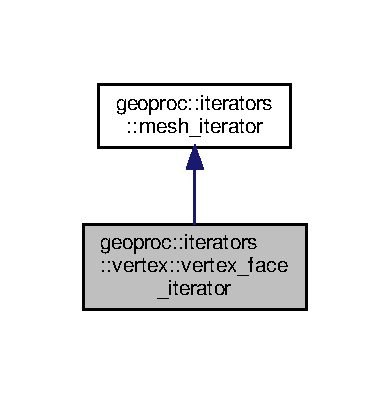
\includegraphics[width=187pt]{classgeoproc_1_1iterators_1_1vertex_1_1vertex__face__iterator__inherit__graph}
\end{center}
\end{figure}


Collaboration diagram for geoproc\+:\+:iterators\+:\+:vertex\+:\+:vertex\+\_\+face\+\_\+iterator\+:\nopagebreak
\begin{figure}[H]
\begin{center}
\leavevmode
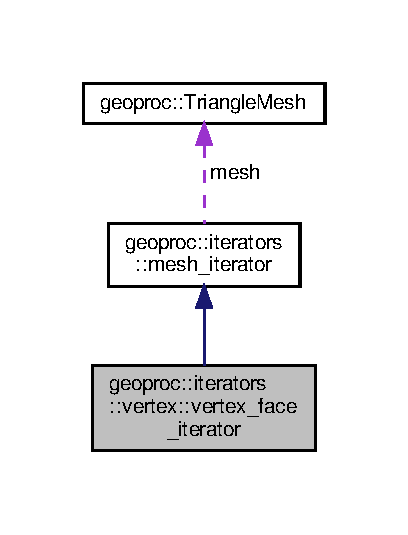
\includegraphics[width=196pt]{classgeoproc_1_1iterators_1_1vertex_1_1vertex__face__iterator__coll__graph}
\end{center}
\end{figure}
\subsection*{Public Member Functions}
\begin{DoxyCompactItemize}
\item 
\hyperlink{classgeoproc_1_1iterators_1_1vertex_1_1vertex__face__iterator_ad45cd64b9e5a3321ac6344984c7cf564}{vertex\+\_\+face\+\_\+iterator} (const \hyperlink{classgeoproc_1_1TriangleMesh}{Triangle\+Mesh} \&m)
\begin{DoxyCompactList}\small\item\em Default constructor. \end{DoxyCompactList}\item 
\mbox{\Hypertarget{classgeoproc_1_1iterators_1_1vertex_1_1vertex__face__iterator_ad3c9661cf4eeb062fd22fc0f4820ba2c}\label{classgeoproc_1_1iterators_1_1vertex_1_1vertex__face__iterator_ad3c9661cf4eeb062fd22fc0f4820ba2c}} 
\hyperlink{classgeoproc_1_1iterators_1_1vertex_1_1vertex__face__iterator_ad3c9661cf4eeb062fd22fc0f4820ba2c}{$\sim$vertex\+\_\+face\+\_\+iterator} ()
\begin{DoxyCompactList}\small\item\em Destructor. \end{DoxyCompactList}\item 
int \hyperlink{classgeoproc_1_1iterators_1_1vertex_1_1vertex__face__iterator_a713d8d9edb7121c729b5717261fd8b3b}{init} (int v)
\begin{DoxyCompactList}\small\item\em Initialise iterator at a vertex. \end{DoxyCompactList}\item 
int \hyperlink{classgeoproc_1_1iterators_1_1vertex_1_1vertex__face__iterator_aa75fe423e210cf4e20e721307c80f6fb}{current} () const
\begin{DoxyCompactList}\small\item\em Returns the current index of vertex. \end{DoxyCompactList}\item 
int \hyperlink{classgeoproc_1_1iterators_1_1vertex_1_1vertex__face__iterator_aa2a7fb3ee7e703d815e7f1664fbd99d4}{next} ()
\begin{DoxyCompactList}\small\item\em Returns the next face. \end{DoxyCompactList}\end{DoxyCompactItemize}
\subsection*{Protected Attributes}
\begin{DoxyCompactItemize}
\item 
\mbox{\Hypertarget{classgeoproc_1_1iterators_1_1mesh__iterator_a6102e0c43bcf7008597387a2f085ca0e}\label{classgeoproc_1_1iterators_1_1mesh__iterator_a6102e0c43bcf7008597387a2f085ca0e}} 
const \hyperlink{classgeoproc_1_1TriangleMesh}{Triangle\+Mesh} \& \hyperlink{classgeoproc_1_1iterators_1_1mesh__iterator_a6102e0c43bcf7008597387a2f085ca0e}{mesh}
\begin{DoxyCompactList}\small\item\em Constant reference to iterated mesh. \end{DoxyCompactList}\end{DoxyCompactItemize}
\subsection*{Private Attributes}
\begin{DoxyCompactItemize}
\item 
\mbox{\Hypertarget{classgeoproc_1_1iterators_1_1vertex_1_1vertex__face__iterator_a3e59b193d3d83c32a803528a0661672b}\label{classgeoproc_1_1iterators_1_1vertex_1_1vertex__face__iterator_a3e59b193d3d83c32a803528a0661672b}} 
int \hyperlink{classgeoproc_1_1iterators_1_1vertex_1_1vertex__face__iterator_a3e59b193d3d83c32a803528a0661672b}{cur\+\_\+corner}
\begin{DoxyCompactList}\small\item\em Current corner index. \end{DoxyCompactList}\item 
\mbox{\Hypertarget{classgeoproc_1_1iterators_1_1vertex_1_1vertex__face__iterator_ac7cecb32cc46b910764b56b977ca8366}\label{classgeoproc_1_1iterators_1_1vertex_1_1vertex__face__iterator_ac7cecb32cc46b910764b56b977ca8366}} 
int \hyperlink{classgeoproc_1_1iterators_1_1vertex_1_1vertex__face__iterator_ac7cecb32cc46b910764b56b977ca8366}{cur\+\_\+face}
\begin{DoxyCompactList}\small\item\em Current face index. \end{DoxyCompactList}\end{DoxyCompactItemize}


\subsection{Detailed Description}
Face iterator class. 

Iterates over the faces on the 1-\/ring neighbourhood of a given vertex. These are the faces adjacent to the given vertex. 

\subsection{Constructor \& Destructor Documentation}
\mbox{\Hypertarget{classgeoproc_1_1iterators_1_1vertex_1_1vertex__face__iterator_ad45cd64b9e5a3321ac6344984c7cf564}\label{classgeoproc_1_1iterators_1_1vertex_1_1vertex__face__iterator_ad45cd64b9e5a3321ac6344984c7cf564}} 
\index{geoproc\+::iterators\+::vertex\+::vertex\+\_\+face\+\_\+iterator@{geoproc\+::iterators\+::vertex\+::vertex\+\_\+face\+\_\+iterator}!vertex\+\_\+face\+\_\+iterator@{vertex\+\_\+face\+\_\+iterator}}
\index{vertex\+\_\+face\+\_\+iterator@{vertex\+\_\+face\+\_\+iterator}!geoproc\+::iterators\+::vertex\+::vertex\+\_\+face\+\_\+iterator@{geoproc\+::iterators\+::vertex\+::vertex\+\_\+face\+\_\+iterator}}
\subsubsection{\texorpdfstring{vertex\+\_\+face\+\_\+iterator()}{vertex\_face\_iterator()}}
{\footnotesize\ttfamily geoproc\+::iterators\+::vertex\+::vertex\+\_\+face\+\_\+iterator\+::vertex\+\_\+face\+\_\+iterator (\begin{DoxyParamCaption}\item[{const \hyperlink{classgeoproc_1_1TriangleMesh}{Triangle\+Mesh} \&}]{m }\end{DoxyParamCaption})}



Default constructor. 


\begin{DoxyParams}{Parameters}
{\em m} & Constant reference to the iterated mesh. \\
\hline
\end{DoxyParams}
\begin{DoxyPrecond}{Precondition}
The mesh requires\+:
\begin{DoxyItemize}
\item Neighbourhood data (see \hyperlink{classgeoproc_1_1TriangleMesh_a84003dfdfd5e591c00f01a797578ff1f}{Triangle\+Mesh\+::make\+\_\+neighbourhood\+\_\+data}) 
\end{DoxyItemize}
\end{DoxyPrecond}


\subsection{Member Function Documentation}
\mbox{\Hypertarget{classgeoproc_1_1iterators_1_1vertex_1_1vertex__face__iterator_aa75fe423e210cf4e20e721307c80f6fb}\label{classgeoproc_1_1iterators_1_1vertex_1_1vertex__face__iterator_aa75fe423e210cf4e20e721307c80f6fb}} 
\index{geoproc\+::iterators\+::vertex\+::vertex\+\_\+face\+\_\+iterator@{geoproc\+::iterators\+::vertex\+::vertex\+\_\+face\+\_\+iterator}!current@{current}}
\index{current@{current}!geoproc\+::iterators\+::vertex\+::vertex\+\_\+face\+\_\+iterator@{geoproc\+::iterators\+::vertex\+::vertex\+\_\+face\+\_\+iterator}}
\subsubsection{\texorpdfstring{current()}{current()}}
{\footnotesize\ttfamily int geoproc\+::iterators\+::vertex\+::vertex\+\_\+face\+\_\+iterator\+::current (\begin{DoxyParamCaption}{ }\end{DoxyParamCaption}) const\hspace{0.3cm}{\ttfamily [virtual]}}



Returns the current index of vertex. 

\begin{DoxyPrecond}{Precondition}
This method must be called after initialising the iteratior with \hyperlink{classgeoproc_1_1iterators_1_1vertex_1_1vertex__face__iterator_a713d8d9edb7121c729b5717261fd8b3b}{init}, and after having called, at least, method \hyperlink{classgeoproc_1_1iterators_1_1vertex_1_1vertex__face__iterator_aa2a7fb3ee7e703d815e7f1664fbd99d4}{next} once. 
\end{DoxyPrecond}
\begin{DoxyReturn}{Returns}
Returns the face index last returned by method \hyperlink{classgeoproc_1_1iterators_1_1vertex_1_1vertex__face__iterator_aa2a7fb3ee7e703d815e7f1664fbd99d4}{next}. 
\end{DoxyReturn}


Implements \hyperlink{classgeoproc_1_1iterators_1_1mesh__iterator_ae6151b065602980d37a582977083ef42}{geoproc\+::iterators\+::mesh\+\_\+iterator}.

\mbox{\Hypertarget{classgeoproc_1_1iterators_1_1vertex_1_1vertex__face__iterator_a713d8d9edb7121c729b5717261fd8b3b}\label{classgeoproc_1_1iterators_1_1vertex_1_1vertex__face__iterator_a713d8d9edb7121c729b5717261fd8b3b}} 
\index{geoproc\+::iterators\+::vertex\+::vertex\+\_\+face\+\_\+iterator@{geoproc\+::iterators\+::vertex\+::vertex\+\_\+face\+\_\+iterator}!init@{init}}
\index{init@{init}!geoproc\+::iterators\+::vertex\+::vertex\+\_\+face\+\_\+iterator@{geoproc\+::iterators\+::vertex\+::vertex\+\_\+face\+\_\+iterator}}
\subsubsection{\texorpdfstring{init()}{init()}}
{\footnotesize\ttfamily int geoproc\+::iterators\+::vertex\+::vertex\+\_\+face\+\_\+iterator\+::init (\begin{DoxyParamCaption}\item[{int}]{v }\end{DoxyParamCaption})\hspace{0.3cm}{\ttfamily [virtual]}}



Initialise iterator at a vertex. 

Modifies this class so that \hyperlink{classgeoproc_1_1iterators_1_1vertex_1_1vertex__face__iterator_aa75fe423e210cf4e20e721307c80f6fb}{current} returns the first face on the 1-\/ring neighbourhood of {\itshape v}.


\begin{DoxyParams}{Parameters}
{\em v} & Index of the vertex. Must be a valid vertex index\+: 0 $<$= {\itshape v} $<$ number of vertices. \\
\hline
\end{DoxyParams}
\begin{DoxyReturn}{Returns}
Returns the first iterated face index. If this value is not collected, call \hyperlink{classgeoproc_1_1iterators_1_1vertex_1_1vertex__face__iterator_aa75fe423e210cf4e20e721307c80f6fb}{current}, before calling \hyperlink{classgeoproc_1_1iterators_1_1vertex_1_1vertex__face__iterator_aa2a7fb3ee7e703d815e7f1664fbd99d4}{next}. 
\end{DoxyReturn}


Implements \hyperlink{classgeoproc_1_1iterators_1_1mesh__iterator_a8a4d8b5c84941dd0a7cb7373abcd3fcc}{geoproc\+::iterators\+::mesh\+\_\+iterator}.

\mbox{\Hypertarget{classgeoproc_1_1iterators_1_1vertex_1_1vertex__face__iterator_aa2a7fb3ee7e703d815e7f1664fbd99d4}\label{classgeoproc_1_1iterators_1_1vertex_1_1vertex__face__iterator_aa2a7fb3ee7e703d815e7f1664fbd99d4}} 
\index{geoproc\+::iterators\+::vertex\+::vertex\+\_\+face\+\_\+iterator@{geoproc\+::iterators\+::vertex\+::vertex\+\_\+face\+\_\+iterator}!next@{next}}
\index{next@{next}!geoproc\+::iterators\+::vertex\+::vertex\+\_\+face\+\_\+iterator@{geoproc\+::iterators\+::vertex\+::vertex\+\_\+face\+\_\+iterator}}
\subsubsection{\texorpdfstring{next()}{next()}}
{\footnotesize\ttfamily int geoproc\+::iterators\+::vertex\+::vertex\+\_\+face\+\_\+iterator\+::next (\begin{DoxyParamCaption}{ }\end{DoxyParamCaption})\hspace{0.3cm}{\ttfamily [virtual]}}



Returns the next face. 

The face index returned is in the 1-\/ring neighbourhood of the vertex used to initialise the iterator (see \hyperlink{classgeoproc_1_1iterators_1_1vertex_1_1vertex__face__iterator_a713d8d9edb7121c729b5717261fd8b3b}{init}).

The order of the faces is guaranteed to be counterclockwise.

\begin{DoxyPrecond}{Precondition}
This method must be called after initialising the iteratior with \hyperlink{classgeoproc_1_1iterators_1_1vertex_1_1vertex__face__iterator_a713d8d9edb7121c729b5717261fd8b3b}{init}. 
\end{DoxyPrecond}
\begin{DoxyReturn}{Returns}
Returns a valid face index. 
\end{DoxyReturn}


Implements \hyperlink{classgeoproc_1_1iterators_1_1mesh__iterator_a32f1ddc2f83743a2b0a4633506601cfe}{geoproc\+::iterators\+::mesh\+\_\+iterator}.



The documentation for this class was generated from the following files\+:\begin{DoxyCompactItemize}
\item 
geoproc/iterators/vertex\+\_\+iterators.\+hpp\item 
geoproc/iterators/vertex\+\_\+iterators.\+cpp\end{DoxyCompactItemize}

\hypertarget{classgeoproc_1_1iterators_1_1vertex_1_1vertex__vertex__iterator}{}\section{geoproc\+:\+:iterators\+:\+:vertex\+:\+:vertex\+\_\+vertex\+\_\+iterator Class Reference}
\label{classgeoproc_1_1iterators_1_1vertex_1_1vertex__vertex__iterator}\index{geoproc\+::iterators\+::vertex\+::vertex\+\_\+vertex\+\_\+iterator@{geoproc\+::iterators\+::vertex\+::vertex\+\_\+vertex\+\_\+iterator}}


Vertex iterator class.  




{\ttfamily \#include $<$vertex\+\_\+iterators.\+hpp$>$}



Inheritance diagram for geoproc\+:\+:iterators\+:\+:vertex\+:\+:vertex\+\_\+vertex\+\_\+iterator\+:\nopagebreak
\begin{figure}[H]
\begin{center}
\leavevmode
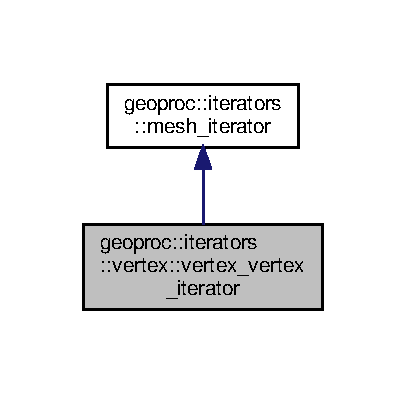
\includegraphics[width=195pt]{classgeoproc_1_1iterators_1_1vertex_1_1vertex__vertex__iterator__inherit__graph}
\end{center}
\end{figure}


Collaboration diagram for geoproc\+:\+:iterators\+:\+:vertex\+:\+:vertex\+\_\+vertex\+\_\+iterator\+:\nopagebreak
\begin{figure}[H]
\begin{center}
\leavevmode
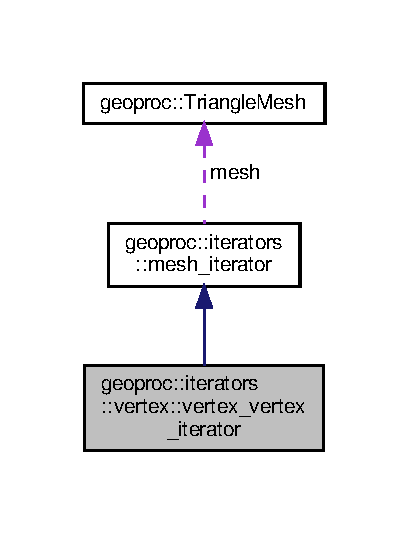
\includegraphics[width=196pt]{classgeoproc_1_1iterators_1_1vertex_1_1vertex__vertex__iterator__coll__graph}
\end{center}
\end{figure}
\subsection*{Public Member Functions}
\begin{DoxyCompactItemize}
\item 
\hyperlink{classgeoproc_1_1iterators_1_1vertex_1_1vertex__vertex__iterator_a6132b060a09bd87279957cc9744cd9af}{vertex\+\_\+vertex\+\_\+iterator} (const \hyperlink{classgeoproc_1_1TriangleMesh}{Triangle\+Mesh} \&m)
\begin{DoxyCompactList}\small\item\em Default constructor. \end{DoxyCompactList}\item 
\mbox{\Hypertarget{classgeoproc_1_1iterators_1_1vertex_1_1vertex__vertex__iterator_a72bd7a8a23b7418d4a6c55fa9e277d08}\label{classgeoproc_1_1iterators_1_1vertex_1_1vertex__vertex__iterator_a72bd7a8a23b7418d4a6c55fa9e277d08}} 
\hyperlink{classgeoproc_1_1iterators_1_1vertex_1_1vertex__vertex__iterator_a72bd7a8a23b7418d4a6c55fa9e277d08}{$\sim$vertex\+\_\+vertex\+\_\+iterator} ()
\begin{DoxyCompactList}\small\item\em Destructor. \end{DoxyCompactList}\item 
int \hyperlink{classgeoproc_1_1iterators_1_1vertex_1_1vertex__vertex__iterator_aa25d74c5f4067074ed6926a6d23800b4}{init} (int v)
\begin{DoxyCompactList}\small\item\em Initialise iterator at a vertex. \end{DoxyCompactList}\item 
int \hyperlink{classgeoproc_1_1iterators_1_1vertex_1_1vertex__vertex__iterator_a3e1a4cd5c67b262156017489662ecabc}{current} () const
\begin{DoxyCompactList}\small\item\em Returns the current index of vertex. \end{DoxyCompactList}\item 
int \hyperlink{classgeoproc_1_1iterators_1_1vertex_1_1vertex__vertex__iterator_ad2041720a1d35892804c659de7b2dd44}{next} ()
\begin{DoxyCompactList}\small\item\em Returns the next vertex. \end{DoxyCompactList}\end{DoxyCompactItemize}
\subsection*{Protected Attributes}
\begin{DoxyCompactItemize}
\item 
\mbox{\Hypertarget{classgeoproc_1_1iterators_1_1mesh__iterator_a6102e0c43bcf7008597387a2f085ca0e}\label{classgeoproc_1_1iterators_1_1mesh__iterator_a6102e0c43bcf7008597387a2f085ca0e}} 
const \hyperlink{classgeoproc_1_1TriangleMesh}{Triangle\+Mesh} \& \hyperlink{classgeoproc_1_1iterators_1_1mesh__iterator_a6102e0c43bcf7008597387a2f085ca0e}{mesh}
\begin{DoxyCompactList}\small\item\em Constant reference to iterated mesh. \end{DoxyCompactList}\end{DoxyCompactItemize}
\subsection*{Private Attributes}
\begin{DoxyCompactItemize}
\item 
\mbox{\Hypertarget{classgeoproc_1_1iterators_1_1vertex_1_1vertex__vertex__iterator_a76628cb7b70644f2e1804c5ea52c94f7}\label{classgeoproc_1_1iterators_1_1vertex_1_1vertex__vertex__iterator_a76628cb7b70644f2e1804c5ea52c94f7}} 
int \hyperlink{classgeoproc_1_1iterators_1_1vertex_1_1vertex__vertex__iterator_a76628cb7b70644f2e1804c5ea52c94f7}{cur\+\_\+corner}
\begin{DoxyCompactList}\small\item\em Current corner index. \end{DoxyCompactList}\item 
\mbox{\Hypertarget{classgeoproc_1_1iterators_1_1vertex_1_1vertex__vertex__iterator_a94e6bf674777a2e825678df7aba64ebd}\label{classgeoproc_1_1iterators_1_1vertex_1_1vertex__vertex__iterator_a94e6bf674777a2e825678df7aba64ebd}} 
int \hyperlink{classgeoproc_1_1iterators_1_1vertex_1_1vertex__vertex__iterator_a94e6bf674777a2e825678df7aba64ebd}{cur\+\_\+vertex}
\begin{DoxyCompactList}\small\item\em Current vertex index. \end{DoxyCompactList}\item 
bool \hyperlink{classgeoproc_1_1iterators_1_1vertex_1_1vertex__vertex__iterator_a3e22144ee36c4739d316aca005e17d87}{half\+\_\+step}
\begin{DoxyCompactList}\small\item\em Should we do only half a step? \end{DoxyCompactList}\end{DoxyCompactItemize}


\subsection{Detailed Description}
Vertex iterator class. 

Iterates over the vertices on the 1-\/ring neighbourhood of a given vertex. 

\subsection{Constructor \& Destructor Documentation}
\mbox{\Hypertarget{classgeoproc_1_1iterators_1_1vertex_1_1vertex__vertex__iterator_a6132b060a09bd87279957cc9744cd9af}\label{classgeoproc_1_1iterators_1_1vertex_1_1vertex__vertex__iterator_a6132b060a09bd87279957cc9744cd9af}} 
\index{geoproc\+::iterators\+::vertex\+::vertex\+\_\+vertex\+\_\+iterator@{geoproc\+::iterators\+::vertex\+::vertex\+\_\+vertex\+\_\+iterator}!vertex\+\_\+vertex\+\_\+iterator@{vertex\+\_\+vertex\+\_\+iterator}}
\index{vertex\+\_\+vertex\+\_\+iterator@{vertex\+\_\+vertex\+\_\+iterator}!geoproc\+::iterators\+::vertex\+::vertex\+\_\+vertex\+\_\+iterator@{geoproc\+::iterators\+::vertex\+::vertex\+\_\+vertex\+\_\+iterator}}
\subsubsection{\texorpdfstring{vertex\+\_\+vertex\+\_\+iterator()}{vertex\_vertex\_iterator()}}
{\footnotesize\ttfamily geoproc\+::iterators\+::vertex\+::vertex\+\_\+vertex\+\_\+iterator\+::vertex\+\_\+vertex\+\_\+iterator (\begin{DoxyParamCaption}\item[{const \hyperlink{classgeoproc_1_1TriangleMesh}{Triangle\+Mesh} \&}]{m }\end{DoxyParamCaption})}



Default constructor. 


\begin{DoxyParams}{Parameters}
{\em m} & Constant reference to the iterated mesh. \\
\hline
\end{DoxyParams}
\begin{DoxyPrecond}{Precondition}
The mesh requires\+:
\begin{DoxyItemize}
\item Neighbourhood data (see \hyperlink{classgeoproc_1_1TriangleMesh_a84003dfdfd5e591c00f01a797578ff1f}{Triangle\+Mesh\+::make\+\_\+neighbourhood\+\_\+data}) 
\end{DoxyItemize}
\end{DoxyPrecond}


\subsection{Member Function Documentation}
\mbox{\Hypertarget{classgeoproc_1_1iterators_1_1vertex_1_1vertex__vertex__iterator_a3e1a4cd5c67b262156017489662ecabc}\label{classgeoproc_1_1iterators_1_1vertex_1_1vertex__vertex__iterator_a3e1a4cd5c67b262156017489662ecabc}} 
\index{geoproc\+::iterators\+::vertex\+::vertex\+\_\+vertex\+\_\+iterator@{geoproc\+::iterators\+::vertex\+::vertex\+\_\+vertex\+\_\+iterator}!current@{current}}
\index{current@{current}!geoproc\+::iterators\+::vertex\+::vertex\+\_\+vertex\+\_\+iterator@{geoproc\+::iterators\+::vertex\+::vertex\+\_\+vertex\+\_\+iterator}}
\subsubsection{\texorpdfstring{current()}{current()}}
{\footnotesize\ttfamily int geoproc\+::iterators\+::vertex\+::vertex\+\_\+vertex\+\_\+iterator\+::current (\begin{DoxyParamCaption}{ }\end{DoxyParamCaption}) const\hspace{0.3cm}{\ttfamily [virtual]}}



Returns the current index of vertex. 

\begin{DoxyPrecond}{Precondition}
This method must be called after initialising the iteratior with \hyperlink{classgeoproc_1_1iterators_1_1vertex_1_1vertex__vertex__iterator_aa25d74c5f4067074ed6926a6d23800b4}{init}, and after having called, at least, method \hyperlink{classgeoproc_1_1iterators_1_1vertex_1_1vertex__vertex__iterator_ad2041720a1d35892804c659de7b2dd44}{next} once. 
\end{DoxyPrecond}
\begin{DoxyReturn}{Returns}
Returns the vertex index last returned by method \hyperlink{classgeoproc_1_1iterators_1_1vertex_1_1vertex__vertex__iterator_ad2041720a1d35892804c659de7b2dd44}{next}. 
\end{DoxyReturn}


Implements \hyperlink{classgeoproc_1_1iterators_1_1mesh__iterator_ae6151b065602980d37a582977083ef42}{geoproc\+::iterators\+::mesh\+\_\+iterator}.

\mbox{\Hypertarget{classgeoproc_1_1iterators_1_1vertex_1_1vertex__vertex__iterator_aa25d74c5f4067074ed6926a6d23800b4}\label{classgeoproc_1_1iterators_1_1vertex_1_1vertex__vertex__iterator_aa25d74c5f4067074ed6926a6d23800b4}} 
\index{geoproc\+::iterators\+::vertex\+::vertex\+\_\+vertex\+\_\+iterator@{geoproc\+::iterators\+::vertex\+::vertex\+\_\+vertex\+\_\+iterator}!init@{init}}
\index{init@{init}!geoproc\+::iterators\+::vertex\+::vertex\+\_\+vertex\+\_\+iterator@{geoproc\+::iterators\+::vertex\+::vertex\+\_\+vertex\+\_\+iterator}}
\subsubsection{\texorpdfstring{init()}{init()}}
{\footnotesize\ttfamily int geoproc\+::iterators\+::vertex\+::vertex\+\_\+vertex\+\_\+iterator\+::init (\begin{DoxyParamCaption}\item[{int}]{v }\end{DoxyParamCaption})\hspace{0.3cm}{\ttfamily [virtual]}}



Initialise iterator at a vertex. 

Modifies this class so that \hyperlink{classgeoproc_1_1iterators_1_1vertex_1_1vertex__vertex__iterator_a3e1a4cd5c67b262156017489662ecabc}{current} returns the first vertex on the 1-\/ring neighbourhood of {\itshape v}.


\begin{DoxyParams}{Parameters}
{\em v} & Index of the vertex. Must be a valid vertex index\+: 0 $<$= {\itshape v} $<$ number of vertices. \\
\hline
\end{DoxyParams}
\begin{DoxyReturn}{Returns}
Returns the first iterated vertex index. If this value is not collected, call \hyperlink{classgeoproc_1_1iterators_1_1vertex_1_1vertex__vertex__iterator_a3e1a4cd5c67b262156017489662ecabc}{current}, before calling \hyperlink{classgeoproc_1_1iterators_1_1vertex_1_1vertex__vertex__iterator_ad2041720a1d35892804c659de7b2dd44}{next}. 
\end{DoxyReturn}


Implements \hyperlink{classgeoproc_1_1iterators_1_1mesh__iterator_a8a4d8b5c84941dd0a7cb7373abcd3fcc}{geoproc\+::iterators\+::mesh\+\_\+iterator}.

\mbox{\Hypertarget{classgeoproc_1_1iterators_1_1vertex_1_1vertex__vertex__iterator_ad2041720a1d35892804c659de7b2dd44}\label{classgeoproc_1_1iterators_1_1vertex_1_1vertex__vertex__iterator_ad2041720a1d35892804c659de7b2dd44}} 
\index{geoproc\+::iterators\+::vertex\+::vertex\+\_\+vertex\+\_\+iterator@{geoproc\+::iterators\+::vertex\+::vertex\+\_\+vertex\+\_\+iterator}!next@{next}}
\index{next@{next}!geoproc\+::iterators\+::vertex\+::vertex\+\_\+vertex\+\_\+iterator@{geoproc\+::iterators\+::vertex\+::vertex\+\_\+vertex\+\_\+iterator}}
\subsubsection{\texorpdfstring{next()}{next()}}
{\footnotesize\ttfamily int geoproc\+::iterators\+::vertex\+::vertex\+\_\+vertex\+\_\+iterator\+::next (\begin{DoxyParamCaption}{ }\end{DoxyParamCaption})\hspace{0.3cm}{\ttfamily [virtual]}}



Returns the next vertex. 

The vertex index returned is in the 1-\/ring neighbourhood of the vertex used to initialise the iterator (see \hyperlink{classgeoproc_1_1iterators_1_1vertex_1_1vertex__vertex__iterator_aa25d74c5f4067074ed6926a6d23800b4}{init}).

The order of the vertices is guaranteed to be counterclockwise.

\begin{DoxyPrecond}{Precondition}
This method must be called after initialising the iteratior with \hyperlink{classgeoproc_1_1iterators_1_1vertex_1_1vertex__vertex__iterator_aa25d74c5f4067074ed6926a6d23800b4}{init}. 
\end{DoxyPrecond}
\begin{DoxyReturn}{Returns}
Returns a valid vertex index. 
\end{DoxyReturn}


Implements \hyperlink{classgeoproc_1_1iterators_1_1mesh__iterator_a32f1ddc2f83743a2b0a4633506601cfe}{geoproc\+::iterators\+::mesh\+\_\+iterator}.



\subsection{Member Data Documentation}
\mbox{\Hypertarget{classgeoproc_1_1iterators_1_1vertex_1_1vertex__vertex__iterator_a3e22144ee36c4739d316aca005e17d87}\label{classgeoproc_1_1iterators_1_1vertex_1_1vertex__vertex__iterator_a3e22144ee36c4739d316aca005e17d87}} 
\index{geoproc\+::iterators\+::vertex\+::vertex\+\_\+vertex\+\_\+iterator@{geoproc\+::iterators\+::vertex\+::vertex\+\_\+vertex\+\_\+iterator}!half\+\_\+step@{half\+\_\+step}}
\index{half\+\_\+step@{half\+\_\+step}!geoproc\+::iterators\+::vertex\+::vertex\+\_\+vertex\+\_\+iterator@{geoproc\+::iterators\+::vertex\+::vertex\+\_\+vertex\+\_\+iterator}}
\subsubsection{\texorpdfstring{half\+\_\+step}{half\_step}}
{\footnotesize\ttfamily bool geoproc\+::iterators\+::vertex\+::vertex\+\_\+vertex\+\_\+iterator\+::half\+\_\+step\hspace{0.3cm}{\ttfamily [private]}}



Should we do only half a step? 

In this case it means that we crossed a boundary, and retrieving the next vertex needs a slightly different procedure. 

The documentation for this class was generated from the following files\+:\begin{DoxyCompactItemize}
\item 
geoproc/iterators/vertex\+\_\+iterators.\+hpp\item 
geoproc/iterators/vertex\+\_\+iterators.\+cpp\end{DoxyCompactItemize}

%--- End generated contents ---

% Index
\backmatter
\newpage
\phantomsection
\clearemptydoublepage
\addcontentsline{toc}{chapter}{Index}
\printindex

\end{document}
